\documentclass[a4paper,landscape,twocolumn]{article}
\usepackage[utf8]{inputenc}
\usepackage[LGR,T1]{fontenc}
\usepackage[ngerman,english]{babel}
\usepackage{amsmath}
\usepackage{amssymb}
\usepackage{amsfonts}
\usepackage{amsthm}
\usepackage{csquotes}
\usepackage{faktor}
\usepackage{fancyhdr}
\usepackage[margin=1in]{geometry}
\usepackage{imakeidx} % before hyperref
\usepackage[pdfborder={0 0 0},colorlinks=true,citecolor=red]{hyperref}
\usepackage{mathtools}
\usepackage{stmaryrd}
\usepackage{rotating}
\usepackage{bbold}

\title{Linear Algebra -- Lecture Notes}
\author{Lukas Prokop}
\date{winter term 2015}

\newcommand\meta[3]{This #1 took place on #2 (#3).\par}
\newcommand\abs[1]{|\,#1\,|}
\newcommand\set[1]{\left\{#1\right\}}
\newcommand\setdef[2]{\left\{#1\,\middle|\,#2\right\}}
\newcommand\card[1]{\left|\,#1\,\right|}
\newcommand\divides[2]{#1\,\mid\,#2}
\newcommand\mathspace{\hspace{20pt}}
\newcommand\Q{\mathbb{Q}}
\newcommand\nope{\lightning}
\newcommand\vecfour[4]{\begin{pmatrix} #1 \\ #2 \\ #3 \\ #4 \end{pmatrix}}
\newcommand{\textgreek}[1]{\begingroup\fontencoding{LGR}\selectfont#1\endgroup}

\newtheorem{theorem}{Theorem}
\newtheorem{defi}{Definition}
\newtheorem{ex}{Example}
\newtheorem{rem}{Remark}
\newtheorem{cor}{Corollary}

\DeclareMathOperator\Hom{Hom} % homomorphism
\DeclareMathOperator\End{End} % endomorphism
\DeclareMathOperator\Aut{Aut} % automorphism
\DeclareMathOperator\image{im} % image
\DeclareMathOperator\kernel{ker} % kernel
\DeclareMathOperator\rank{rank} % rank of a matrix

\DeclarePairedDelimiter\norm\lVert\rVert

\setcounter{MaxMatrixCols}{20}

\pagestyle{fancy}
\fancyhf{}
\chead{\Large{\textsc{Linear Algebra I -- Lecture Notes}}}
\lfoot{\makebox[\columnwidth]{\thepage}}
\rfoot{\makebox[\columnwidth]{\number\numexpr\value{page}+1}\stepcounter{page}}
\setlength{\headheight}{18pt}

\parindent0pt
\parskip5pt

\makeindex[name={German},title={German keywords}]
\makeindex[name={English},title={English keywords}]
\twocolumn

\begin{document}
\maketitle
\tableofcontents

\clearpage
\meta{lecture}{5th of Oct 2015}{Prof. Franz Lehner}

Weekly schedule:

\begin{table}[!ht]
  \begin{tabular}{rcl}
    \hline \hline
    Mon & 08:15--09:45 & KF 06.01 \\
    Tue & 08:15--09:45 & TU P2 \\
    Tue & 10:15 & BE 01, Konversatorium \\
    Wed & 13:00--15:00 & UE + Onlinekreuzesystem, Deadline 11:00 \\
    Mon, Tue, Thu & * & Tutorien \\
    \hline \hline
  \end{tabular}
\end{table}

Exams:
\begin{enumerate}
  \item VO-Prüfung (schriftlich, 3 Termine pro Semester, ohne Unterlagen)
  \item 2 UE-Prüfungen (25.11, 27.01, 1 DIN A4 Blatt)
\end{enumerate}

\textbf{What is linear algebra?}
\begin{itemize}
  \item Arithmetics (greek: \textgreek{ἀριθμός})
  \item Geometry (greek: \textgreek{γεωμετρία})
  \item Analysis / infinitesimal computation (greek: \textgreek{ἀνάλυσις})
\end{itemize}

100 years ago, the following branch of mathematics was introduced:
\begin{itemize}
  \item Algebra: abstract computational operations (fields, groups, rings, etc)
  \begin{itemize}
    \item Linear algebra (branch of algebra, related to vector computations)
  \end{itemize}
\end{itemize}

Mathematics is the search for statements of the structure: \emph{If A, then B}.

\section{Set theory, logic and linear equations}
\subsection{Axiomatic definition of a set}

Georg Kantor (1869)
\begin{quote}
  Unter einer Menge verstehen wir eine Zusammenfassung von \emph{bestimmten}
  \emph{wohlunterschiedenen} Objekten unserer Anschauung oder unsres Denkens
  (welche die Objekte der Menge $M$ genannt werden) zu einem Ganzen.
\end{quote}
\begin{quote}
  We define a set as a combination of defined well-distinguishable objects of
  our perception and our minds (which are denoted set $M$) to a whole unit.
\end{quote}

Hence for every object $x$ one of these statements hold:
\begin{itemize}
    \item $x$ is part of $M$: $x \in M$
    \item $x$ is not part of $M$: $x \in M$
\end{itemize}

\subsection{Notation for set theory}

Approaches for notations:
\begin{itemize}
  \item Enumeration
    \begin{itemize}
      \item $\set{1,2, 3}$, $\set{a, b, \text{teddy bear}, \text{lecture hall HS 06.01}}$
      \item Integers (in this lecture: without zero): $\mathbb{N} = \set{0, 1, 2, \ldots}$
      \item $\set{1, 2, 3, \ldots}$: integers, end undetermined
      \item $\set{1, 2, \ldots, n}$: integers from 1 to $n$
      \item $\set{x, y, \ldots, z}$: general finite set
    \end{itemize}
  \item Description
    \begin{itemize}
      \item $\set{1, 4, 9, 16, \ldots}$
      \item $\set{n | n \text{ is square of an integer}}$
      \item $\set{n | \text{there exists } k \in \mathbb{N} \text{ such that } n = k^2} = \set{k^2 | k \in \mathbb{N}}$
    \end{itemize}
  \item Defined set with shortcuts
    \begin{itemize}
      \item $\mathbb{N}$
      \item $\mathbb{Z} = \set{0, \pm 1, \pm 2, \ldots}$
      \item $\mathbb{Q} = \set{\frac{p}{q} | p \in \mathbb{Z}, q \in \mathbb{N}}$
      \item $\mathbb{R} = $ complex definition, see analysis
      \item $\mathbb{C} = \setdef{x + y}{x, y \in \mathbb{R}}$
      \item $\set{} = \emptyset$ as the empty set
      \item M. Bourbaki, \enquote{Elements of mathematics}
    \end{itemize}
\end{itemize}

\subsubsection{Examples for custom sets}

\begin{description}
  \item[\enquote{The set of all competent politicians}]
    Not well-defined, opinion-based
  \item[\enquote{The set of all visible fix stars}]
    Depends on definition of visibility, are tools allowed?, opinion-based
\end{description}

\subsection{Russell's paradox}

\fbox{Bertrand Arthur William Russell, 1872--1970}
\fbox{Ernst Friedrich Ferdinand Zermelo, 1871--1953}

Russell 1901, Zermelo 1902

$M$ = \enquote{the set of all sets} = \enquote{the set of all sets that does not contain itself}

\subsection{Berry's paradox}

$M_{12}$ = set of all integers not definable with fewer than 12 words \\
$n$ is \enquote{the smallest positive integer not definable in fewer than twelve words}

So $n$ is not contained in $M_{12}$. But $n$ itself is now defined with 11 words.
So it's contained? Paradox.

\subsection{Axiomatic system of Zermelo-Frauenkel}

\begin{enumerate}
  \item For all sets $A, B$ it holds that $A = B$ iff $x \in A$ then also $x \in B$.
  \item An empty set exists. Hence for all $x$ it holds that $x \notin \emptyset$.
  \item If $A$ and $B$ are sets, then also $\set{A, B}$.
  \item If $A$ and $B$ are sets, then also the union of  $A \cup B$ is a set.
  \item An infinite set exists.
  \item If $A$ is a set, then also the power set $\mathcal{P}(A) = \set{B | B \subseteq A}$
\end{enumerate}

\subsection{Basics of logic}

Aristoteles (\textgreek{Ἀριστοτέλης}) and Organon (\textgreek{Ὄργανον}).
Organon called the system \enquote{analytics}.

\begin{quote}
  A \emph{statement} is a linguistic unit which is \emph{true} or \emph{false}.
\end{quote}

Examples:
\begin{itemize}
  \item Sokrates is a human.
  \item 7 is a prime number.
  \item 5 is an even number.
  \item There exists only one universe.
\end{itemize}

The last example has an unknown truth value.
Constructivists: \enquote{Unknown means false}.
Pragmatics: \enquote{Unknown means unknown}.

Other examples for unknown truth values:
\begin{itemize}
  \item Today is monday.
  \item A. Gabalier has a beautiful voice.
\end{itemize}

Epimenides
\begin{quote}
  All crets are liars.
\end{quote}

Russell:
\begin{quote}
  This statement is wrong.
\end{quote}

\subsection{Gödel's incompleteness theorem}

Kurt Gödel (1930)
\begin{quote}
  In every formal system statements exist that
  are true, but not provable.
\end{quote}

Example: \enquote{This statement is not provable.}

\subsection{A clarification}

Due to these contradictions:
\begin{quote}
  A \emph{statement} is a linguistic unit for which it makes sense to ask:
  is it \emph{true} or \emph{false}?
\end{quote}

\subsection{Formal logic}

\begin{description}
  \item[Negation]
    $\neg A$ means the truth value of $A$ is inverted
  \item[Conjunction]
    $A \land B$ is true, if $A$ and $B$ is true
\end{description}

Attention!
\begin{itemize}
  \item Eating and drinking forbidden (actually: \enquote{no eating or drinking})
  \item Solutions for $x^2 = 1$: $x_1 = 1$ and $x_2 = -1$ (\enquote{actually: $x_1 = 1$ \emph{or} $x_2 = -1$})
\end{itemize}

\begin{description}
  \item[Disjunction]
    $A \lor B$ is true, if $A$ or $B$ is true (latin \enquote{vel})
  \item[Exclusive disjunction]
    $A \dot\lor B$ is true if $A$ or $B$ but not both are true (latin \enquote{out})
  \item[Equivalence]
    $A \leftrightarrow B$ is true if both share the same truth value ($\neg (A \dot\lor B)$)
  \item[Implication / subjunction]
    $A \implies B$ is true if $A$ is false or $A$ is true and $B$ is false.
    $A$ implies $B$. Deutsch: \enquote{A ist hinreichend für B. B ist notwendig für A.}
\end{description}

\subsection{Definition}

Two logical statements are equivalent if for every variable assignment,
the same truth value is evaluated ($P(A_1, \ldots, A_n) \leftrightarrow Q(A_1, \ldots, A_n)$).

\subsection{Logical laws by DeMorgan}

\begin{align*}
  \neg(A \land B) &\Leftrightarrow \neg A \lor \neg B \\
\end{align*}

\meta{lecture}{6th of Oct 2015}{Prof. Franz Lehner}

\[ \card{\mathbb{N}} = \aleph_0 \]

\subsection{Proofs}

A sentence is a statement of kind:
\[ A \implies B \]

$A$ is our requirement. $B$ is our conclusion.
A proof is showing that $B$ holds under assumption of $A$.

\subsection{Statement}

\begin{quote}
  Let $n \in \mathbb{N}$ be odd, than $n^2$ is odd.
\end{quote}

Proof:
\begin{itemize}
  \item[$A$.] $n$ is even and $n \in \mathbb{N}$, hence there exists some
           $k \in \mathbb{N}_0$ such that $n = 2k + 1$
  \item[$B$.] $n^2$ is odd, hence it holds that $l \in \mathbb{N}_0$ such that
           $n^2 = 2l + 1$
\end{itemize}

We know, $n = 2k + 1$

\[ \Rightarrow n^2 = (2k + 1)^2 = 4k^2 + 4k + 1 = 2\cdot(2k^2 + 2k) + 1 \]
with $l = 2k^2 + 2k$, statement $B$ holds. Direct proof.

\subsubsection{Contraposition law}

\[ A \implies B \Leftrightarrow \neg B \implies \neg A \]

A so-called \enquote{indirect proof}.

\begin{quote}
  If $n^2$ is even, than $n$ is even.
\end{quote}

\begin{itemize}
  \item[$A$.] $n^2$ is even
  \item[$B$.] $n$ is even
  \item[$\neg B$.] $n$ is odd
  \item[$\neg A$.] $n$ is odd
\end{itemize}

We already have shown,

\[ \neg B \implies \neg A \]

hence also $A \implies B$ is true.

\subsection{Proof by contradiction}

\[ A \lor \neg A \]

Tertium nondatur \\
hence if $\neg A$ is false, then $A$ is true.

\subsubsection{$\sqrt{2}$ is irrational}

\[ \sqrt{2} \not\in \mathbb{Q} \]

Proof:

\begin{itemize}
  \item[$A$.] Let $x \in \mathbb{R}$ such that $x^2 = 2$ and $x > 0$ and let $\sqrt{2}$ be that number
  \item[$B$.] $\sqrt{2} \not\in \mathbb{Q}$
\end{itemize}

Assume $\neg B$ hence $\sqrt{2} \in \mathbb{Q}$. We find a contradiction.

$\sqrt{2} \in \mathbb{Q}$ then there exists some $p \in \mathbb{Z}, q \in \mathbb{N}$ such that $\sqrt{2} = \frac{p}{q}$.

Wlog (without loss of generality), we assume that the fraction is irreducible. Hence $\operatorname{gcd}(p, q) = 1$.

Therefore $\sqrt{2}$ has the following property.
\begin{align*}
  \sqrt{2} &= \frac{p}{q} \\
  (\sqrt{2})^2 &= 2 \\
  \frac{p^2}{q^2} &= 2 \\
  \Rightarrow p^2 &= 2 q^2 \\
  \Rightarrow p^2 \text{ is even} \\
  \Rightarrow p \text { is even }
\end{align*}

hence there exists some $k \in \mathbb{N}$ such that $p = 2k$

\begin{align*}
  (2k)^2 &= 2q^2 \\
  4k^2 &= 2q^2 \\
  2k^2 &= q^2 \\
  \Rightarrow q^2 \text{ is even} \\
  \Rightarrow q \text{ is even} \\
\end{align*}

hence there is some $l \in \mathbb{N}$ such that $q = 2l$.

\[ \sqrt{2} = \frac{2k}{2l} \]

is not reduced. This is contradictory to our original statement.

\[ \operatorname{gcd}(p,q) = \operatorname{gcd}(2k, 2l) \]
\[ \geq 2 \neq 1 \]

$\Rightarrow \neg B$ is wrong, so $B$ is true.

\subsection{Remark about constructivism}

A few mathematicians deny \enquote{tertium non datur}.
For those $A \lor \neg A$ means that there is no proof for either statement.

\subsubsection{$a^b$ is irrational with $a, b \in \mathbb{R}$}

Proof: We know that $\sqrt{2} \not\in \mathbb{Q}$.

\[
    \left(\sqrt{2}^{\sqrt{2}}\right)^{\sqrt{2}}
    = \sqrt{2}^{\sqrt{2}\cdot\sqrt{2}}
    = \sqrt{2}^2
    = 2^{\in \mathbb{Q}}
\]

\begin{enumerate}
  \item[case 1:]
    $\sqrt{2}^{\sqrt{2}}$ is irrational
    $\Rightarrow$ choose $a = \sqrt{2}^{\sqrt{2}} \not\in \mathbb{Q},
    b = \sqrt{2} \not\in \mathbb{Q}, a^b \in \mathbb{Q}$
  \item[case 2:]
    $\sqrt{2}^{\sqrt{2}} \in \mathbb{Q}$
    choose $a = \sqrt{2} \not\in \mathbb{Q}$ and $b = \sqrt{2} \not\in \mathbb{Q}$
    and $a^b \in \mathbb{Q}$.
\end{enumerate}

With other means means that $\sqrt{2}^{\sqrt{2}} \not\in \mathbb{Q}$.

\subsection{Agreement}

A \emph{predicate} is an expression which depends on variable and
by insertion of values, a statement is created.

\[ P(n) \Leftrightarrow \text{ $n$ is even} \]

is not a statement unless we define $n$.

\[ P(2) \Leftrightarrow \text{2 is even} \]
\[ P(3) \Leftrightarrow \text{3 is even} \]

\subsection{Quantifiers}

\[ Q(n) \Leftrightarrow \left(P(n = 2k + 1) \implies P(n^2 = 2l + 1)\right) \]

hence the statement
\[ Q(1) \land Q(2) \land Q(3) \land Q(4) \land Q(5) \ldots \]

Notation:
\[ \bigwedge_{n \in \mathbb{N}} Q(n) \:\text{ or }\: \forall n \in \mathbb{N}: Q(n) \]

So we can briefly write:
\[ \bigwedge_{n \in \mathbb{N}} Q(n) \]
meaning for all $n \in \mathbb{N}$ it holds that \enquote{$n$ is odd implies $n^2$ is odd}.

$\bigwedge$ is called \enquote{all quantifier}.

Analogously for $P(1) \lor P(2) \lor P(3) \lor \ldots$ is true if there is some $n$ such that $P(n)$ is true.

\[ \bigvee_{n \in \mathbb{N}} P(n) \Leftrightarrow \exists n: P(n) \]

Variant:
\[ \dot\bigvee_{x \in X} P(x) \]

there exists \emph{exactly one} $x$ such that $P(x)$ holds.

\[ \exists! x \in X: P(x) \]

\subsection{Proof using quantifiers}

There exists some prime number:

\begin{itemize}
  \item $\bigwedge_{n \in \mathbb{N}} n \in \mathbb{P}$
        where $\mathbb{P}$ is the set of prime numbers.
  \item An integer is a prime number, if it does not have real divisor.
        \[
            \divides{k}{n} \: = \text{$k$ divides $n$}
            \Leftrightarrow \bigvee_{l \in \mathbb{N}} k\cdot l = n
        \] \[
            \bigwedge_{n \in \mathbb{N}} n \in \mathbb{P}
              \leftrightarrow \neg \bigvee_{k \in \mathbb{N}} (k > 1) \land (k < n) \land (\divides{k}{n})
        \]
\end{itemize}

\subsection{Negation with quantifiers}

\[ \neg(A \land B) \Leftrightarrow \neg A \lor \neg B \]
\[ \neg \bigwedge_{x \in X} P(x) \Leftrightarrow \bigvee_{x \in X} \neg P(x) \]

\subsection{Relation between set theory and boolean algebra}

\begin{align*}
  A \cap B &= \setdef{x}{x \in A \land x \in B} \\
  A \cup B &= \setdef{x}{x \in A \lor x \in B} \\
  A \triangle B &= \setdef{x}{x \in A \dot\lor x \in B} \mathspace \text{\enquote{symbolic difference}} \\
  A \setminus B &= \setdef{x}{x \in A \land x \notin B}
\end{align*}
\begin{align*}
  A^C &= \setdef{x \in U}{x \not\in A} \mathspace \text{\enquote{complement in $U$, the universe}} \\
      &= U \setminus A \\
  A \subseteq B &\Leftrightarrow \bigwedge_{x \in A} x \in B \\
                &\Leftrightarrow \bigwedge_{x} \left(x \in A \implies x \in B\right) \\
  A = B &\Leftrightarrow \bigwedge_x x \in A \Leftrightarrow x \in B
\end{align*}

Let $A_i$ with $i \in I$ (where $I$ is the index set) be sets than
\[ \bigcap_{i \in I} A_i = \setdef{x}{\bigwedge_{i \in I} x \in A_i} \mathspace \text{intersection of all $A_i$} \]
\[ \bigcup_{i \in I} A_i = \setdef{x}{\bigvee_i x \in A_i} \mathspace \text{union of all $A_i$} \]

\[
    \bigcap_{i \in I} A_i \cap \bigcap_{j \in J} A_j
    = \bigcap_{i \in I \cup J} A_i
    = \setdef{x}{\bigwedge_{i \in I \cup J} x \in A_i}
\]

What happens at $I = \emptyset$?
\[ \bigwedge_{x \in \emptyset} P(x) \Leftrightarrow W \mathspace\text{is always true} \]

This is axiomatic:
\[ \bigwedge_{x \in \emptyset} P(x) \mathspace \text{is always true} \]

$I = \mathbb{R}$, for every $x \in \mathbb{R}$ a set $A_x$ is given
\[ \bigcap_{x \in \mathbb{R}} A_x = \setdef{y}{\bigwedge_{x \in \mathbb{R}} y \in A_x} \]
\[ \bigvee_{x \in \emptyset} Q(x) \mathspace\text{is always false} \]

\section{Power sets}

Let $A$ be a set.
\[ P(A) = 2^A = \setdef{B}{B \subseteq A} \]
is called a \enquote{power set} of $A$.

\[ P(\emptyset) = \set{\emptyset} \]
\[ P(P(\emptyset)) = \set{\emptyset, \set{\emptyset}} \]

Let $A, B$ be sets.
The following set is called \enquote{cartesian product} (lat. renatus cartesius) (by René Descartes, 17th century)
\[ A \times B = \setdef{(a, b)}{a \in A, b \in B} \]

Followingly,
\begin{align*}
  A^2 &= A \times A \\
  A^n &= \underbrace{A \times A \times \ldots}_{n} \\
  A \times B \times C &= \setdef{(a, b, c)}{a \in A, b \in B, c \in C} \\
  A^n &= \setdef{(a_1, \ldots, a_n)}{a_i \in A} \\
  A^I &= \setdef{(a_i)_{i \in I}}{a_i \in A}
\end{align*}

3ary tuples are called \enquote{triples}.
$(a_i)_{i \in I}$ is called family of elements (where $I$ is an index set).

\section{Relations of sets}

A \emph{relation} on a set is a subset
\[ R \subseteq X \times X \]

Notation: $x R y$ means $x$ is in relation with $y$. Hence $(x, y) \in R$.

Example: $X$ is the set of austrians. The relation is marriage.
  Be aware that every married couple occurs twice. Once as $(x, y)$ and once as $(y, x)$.

\meta{lecture}{12th of Oct 2015}{Prof. Franz Lehner}

A relation of a set $X$ is a subset $R \subseteq X \times X$. We denote $x R y$ iff $(x,y) \in R$.

\begin{table}[!ht]
  \begin{center}
    \begin{tabular}{crlccccc}
     \hline \hline
      i & set & $R$ \\
     \hline
      0 & $X = \set{\text{Austrian}}$ & \enquote{married} \\
      1 & $X = \set{\text{Austrian}}$ & same location of birth \\
      2 & $X = \mathbb{R}$ & $x \leq y$ \\
      3 & $X$ arbitrary & $x = y$ \\
      4 & $X = \mathbb{N}$ & $\divides{x}{y}$ \\
      5 & $X = \mathbb{Z}, \text{defined } n \in \mathbb{N}$ & $\divides{n}{x - y}$ \\
      6 & $X = \set{a, b, c}$ & $R = \set{(a, a), (a, c), (b, b), (c, a), (c, c)}$ \\
     \hline \hline
    \end{tabular} \\[5pt]
    \begin{tabular}{crlccccc}
     \hline \hline
        i & reflexive & symmetrical & anti-sym. & transitive & konnex \\
     \hline
        0 & false & true & false & false & false \\
        1 & true & true & false & true & false \\
        2 & true & false & true & true & true \\
        3 & true & true & true & true & false \\
        4 & true & false & true & true & false \\
        5 & true & true & false & true & false \\
        6 & true & true & false & true & false \\
     \hline \hline
    \end{tabular}
    \caption{Examples for relations and their properties}
  \end{center}
\end{table}

A \emph{relation} $R$ operating on a set $X$ is called
\begin{description}
  \item[reflexive] \hfill{} \\
    if $\bigwedge_{x \in X} x R x$ (hence $(x, x) \in \mathbb{R}$)
  \item[symmetrical] \hfill{} \\
    if $\bigwedge_{x \in X}{y \in X} \left(xRy \implies yRx\right)$
  \item[anti-symmetrical] \hfill{} \\
    if $\bigwedge_{x \in X} \bigwedge_{y \in X} (xRy \land yRx \implies x=y)$
  \item[transitive] \hfill{} \\
    if $\bigwedge_{x \in X} \bigwedge_{y \in X} \bigwedge_{z \in X} (xRy \land yRz) \implies xRz$
  \item[konnvex] \hfill{} \\
    if $\bigwedge_{x \in X} \bigwedge_{y \in X} (xRy \lor yRx)$
\end{description}

A relation satisfying reflexivity, symmetry and transitivity is called \emph{equivalence relation}.
Examples 2, 4, 6 and 7 are equivalence relations.

A relation satisfying reflexivity, anti-symmetry and transitivity is called \emph{order relation}.
Examples 3, 4 and 5 are order relations.

A relation satisfying reflexivity, anti-symmetry, transitivity and konnvexivity is called \emph{total order}.
Example 2 is a total order.

Let $\sim$ be an equivalence relation operating on set $X$.
For $x \in X$,
\[ [x] = \setdef{y \in X}{x \sim y} \]
is called equivalence class of $x$.

Examples:
\begin{itemize}
  \item $[x] = \setdef{y}{y \text{ has the same location of birth}}$
  \item $[x] = \setdef{y}{x = y} = \set{x}$
  \item $[x] = \setdef{y}{\divides{n}{x - y}} = \setdef{y}{x - y = q\cdot n} = \setdef{y}{y = x - q \cdot n} = \setdef{x + k \cdot n}{k \in \mathbb{Z}}$
  \item $[a] = \set{a, c}, [b] = \set{b}, [c] = \set{a, c}$
\end{itemize}

$\faktor{X}{\sim} = \setdef{[x]}{x = X}$ is called \emph{factor set} or \emph{quotient set}.

Examples:
\begin{itemize}
  \item $\faktor{X}{\sim} = \set{\set{\text{Graz}}, \set{\text{Linz}}, \set{\text{Wien}}, \dots}$
  \item $\faktor{X}{\sim} = \setdef{\set{x}}{x \in X}$
  \item $\mathbb{Z}{\sim} = \set{[0], [1], [2], \ldots, [n-1]}$
     \[ n = 0 + 1 \cdot n \in [0] \]
     \[ 0 = n - 1 \cdot n \in [n] \]
\end{itemize}

A \emph{system of representatives} is a subset $S \subseteq X$ such that
\[ \bigwedge_{[x] \in \faktor{X}{\sim}} \dot\bigvee_{s \in S} s \in [x] \]

Examples:
\begin{itemize}
  \item The mayor of a city.
  \item $S = X$
  \item $S = \set{0, \ldots, n - 1}$
\end{itemize}

\begin{theorem}
  \label{satz-1.2.9}
  Let $\sim$ be an equivalence relation operating on $X$.
  Then it holds that
  \[ \bigwedge_{x,y \in X} \left(x \sim y \iff [x] = [y]\right) \]
\end{theorem}

Proof:
Let $x,y \in X$ be arbitrary elements such that $x \sim y$.
Show that $[x] \subseteq [y] \land [y] \subseteq [x]$.
It suffices to show that $[x] \subseteq [y]$ because $x,y$ can be arbitrary.

Show $\bigwedge_{z \in [x]} z \in [y]$.
Let $z \in [x] \implies x \sim z$. Furthermore $x \sim y \xrightarrow{symmetrical} y \sim x$.
Hence $y \sim x \land x \sim z \xrightarrow{transitive} y \sim z \implies z \in [y]$.
Hence $[x] \subseteq [y]$. Hence $[x] = [y]$.

If $[x] = [y]$, then $y \in [y]$ (because its reflexive) hence $y \in [x] \implies x \sim y$.

Let $X$ be a set. A \emph{partition} of $X$ is a subset $Z \subseteq \mathcal{P}(X)$.
$Z$ is the set of subsets of $X$ such that

\begin{itemize}
  \item $\bigcup_{A = Z} A = X$
  \item $\bigwedge_{A,B \in Z} \left(A \neq B \implies A \cap B = \emptyset\right)$
    \[ \iff \bigwedge_{x \in X} \bigvee_{A \in Z} x \in A \]
\end{itemize}

\begin{theorem}
  Let $X$ be a non-empty set.
  \begin{itemize}
    \item
      Let $\sim$ be an equivalence relation operating on $X$,
      then $\faktor{X}{\sim}$ is a partition of $X$.
    \item
      Let $Z \subseteq \mathcal{P}(X)$ a partition of $X$.
      There is exactly one equivalence relation $\sim$ on $X$
      such that $\faktor{X}{\sim} = Z$.
  \end{itemize}
\end{theorem}

\begin{proof}
  Let $\sim$ be an equivalence relation on $X$.
  Then $\faktor{X}{\sim} = \setdef{[x]}{x \in X} \subseteq \mathcal{P}(x)$

  \begin{itemize}
    \item We need to show that $\bigcup_{x \in X} [x] = X$.
      \begin{align*}
        \bigwedge_{x \in X} x \sim y &\implies \bigwedge_{x \in X} x \in [x] \\
                                   &\implies \bigwedge_{x \in X} x \in \bigcup_{y \in X} [y] \\
                                   &\implies X \subseteq \bigcup_{y \in X} [y]
      \end{align*}
    \item Furthermore we need to show that
          $\bigwedge_{x,y \in X} [x] \cap [y] \neq \emptyset \implies [x] = [y] \iff x \sim y$.
      \begin{align*}
          \text{Let } [x] \cap [y] \neg \emptyset & \bigvee_z z \in [x] \cap [y] \\
              & \bigvee_z z \in [x] \land z \in [y] \\
          \text{definition of equivalence class} & \implies x \sim z \land y \sim z \\
          \text{symmetrical} & \implies \bigvee_z x \sim z \land z \sim y \\
          & \xrightarrow{transitive} x \sim y \\
          & \xrightarrow{Theorem~\ref{satz-1.2.9}} [x] = [y]
      \end{align*}
  \end{itemize}
\end{proof}

\meta{lecture}{13rd of Oct 2015}{Prof. Franz Lehner}

A \emph{function} (or mapping) between two sets $X$ and $Y$
\[ f: X \rightarrow Y \]
\[ x \mapsto f(x) \]
is a relation assigning every element $x \in X$ some $f(x) \in Y$.

$X$ is called domain and $Y$ is called co-domain (also range or image).
$f(x)$ is called image of $x$ under $f$.
We can find a symbolic expression for a function or explicitly enumerate all mappings possibilities.

Examples:
\begin{align*}
  f_1: \mathbb{R} &\rightarrow \mathbb{R} \\
                x &\rightarrow x^2 \\
  f_2: \set{0,1}  &\rightarrow \mathbb{R} \\
                0 &\rightarrow 1
                1 &\rightarrow \pi \\
  f_3: \mathcal{P}(x) &\rightarrow \mathcal{P}(x) \\
                A &\mapsto X \setminus A
\end{align*}

Let $\sim$ be an equivalence relation operating on set $X$.

\begin{align*}
  f_4: X &\rightarrow \faktor{X}{\sim} \\
       x &\mapsto [x] \\
  f_5: \mathbb{R} \times \mathbb{R} &\rightarrow \mathbb{R} \\
       (x,y) &\mapsto x+y
\end{align*}

Remarks:
\begin{enumerate}
  \item
    Domain and codomain are part of the definition of a function.
    A function is unambiguously defined by some graph:

  \item
    \[ G_f = \setdef{(x, f(x))}{x \in X} \subseteq X \times Y \]
    therefore a relation between $X$ and $Y$ such that every $x \in X$
    occurs exactly once.
    \[ \bigwedge_{x\in X} \dot\bigvee_{y\in Y} (x,y) \in G_f \]

  \item
    Two functions $f: X \rightarrow Y$, $f: U \rightarrow V$ are
    equivalent iff $X = U$, $Y = V$ and $\bigwedge_{x \in X} f(x) = g(x)$.

    Hence the domain and codomain must be equivalent.

  \item
    The function $\text{id}_X: X \rightarrow X$ is called \enquote{identity}.

  \item
    Let $A \subseteq X$ be a subset.
    \[ \mathbb{1}_A = \chi_A: X \rightarrow \set{0,1} \]
    \[
       x \rightarrow \begin{cases}
         1 & \text{if } x \in A \\
         0 & \text{if } x \notin A
       \end{cases}
    \]
    This function is called \emph{indicator function of $A$}
    or \emph{characteristic function of $A$}.

  \item
    Every function $f: X \rightarrow \set{0,1}$ is the indicator
    function of a subset of $X$, namely $f = \mathbb{1}_A$
    where $A = \setdef{x \in X}{f(x) = 1}$.
\end{enumerate}

Let $A \subseteq X$ be a subset of $f: X \rightarrow Y$.
Then $f\mid_A: A \rightarrow Y$ with $a \mapsto f(a)$ is
called \emph{restriction} of $f$ to $A$.

$f\mid_A$ is not defined outside $A$.

Let $f: X \rightarrow Y$ be a function defined for $B \subseteq Y$.
\[ f^{-1}(B) = \setdef{x \in X}{f(x) \in B} \subseteq X \]
Therefore we define the domain function
\[ f^{-1}: \mathcal{P}(Y) \rightarrow \mathcal{P}(X) \]

$f^{-1}(B)$ can be empty.

If $B = \set{y}$ then we write $f^{-1}(y)$ instead of $f^{-1}(\set{y})$.
\[ f^{-1}(1) = f^{-1}(\set{1}) = \set{+1, -1} \]
\[ f^{-1}(-1) = \emptyset \]
\[ f(\set{1, 2}) = \set{1,4} \]
\[ f(\set{+1, -1}) = \set{1} \]

Analogously $f$ indicates a function
\[ \tilde f: \mathcal{P}(X) \rightarrow \mathcal{P}(Y) \]
\[ A \mapsto f(A) = \setdef{f(x)}{x \in A} \]

Remark:
\[ f^{-1}(B) = \bigcup_{b \in B} f^{-1}(b) \]

A function $f: X \rightarrow Y$ is called \emph{injective} iff
\[ \bigwedge_{x_1,x_2 \in X} (x_1 \neq x_2 \implies f(x) \neq f(x_2)) \]
\[ \iff \bigwedge_{x_1,x_2 \in X} (f(x_1) = f(x_2) \implies x_1 = x_2) \]

A function is called \emph{surjective} iff
\[ \bigwedge_{y \in Y} \bigvee_{x \in X} f(x) = y \]

A function is called \emph{bijective} iff a function is injective and surjective.
\[ \bigwedge_{y \in Y} \dot\bigvee_{x \in X} f(x) = y \]

For a bijective function $f^{-1}$ is called \emph{inverse function}.
\[ f^{-1}: Y \rightarrow X \]
\[ y \mapsto \text{\small every distinct $x$ such that $f(x) = y$} \]

Be aware that $f^{-1}(y)$ sometimes means $f^{-1}(\set{y})$.

Examples:
\begin{itemize}
  \item
    $f: x \mapsto 3x$ in $\mathbb{R} \rightarrow \mathbb{R}$ is injective and surjective.
    Therefore it is also bijective.
  \item
    $f: x \mapsto x^2$ in $\mathbb{R} \rightarrow \mathbb{R}$ is not injective and not surjective.
    We have a restriction:
    \[ \tilde f: \mathbb{R}_0^+ \rightarrow \mathbb{R}_0^+ \]
    With this domain, the function is bijective.
  \item
    $f: x \mapsto x^3$ in $\mathbb{R} \rightarrow \mathbb{R}$ is bijective.
  \item
    $f: A \mapsto A^C = X \setminus A$ in $\mathcal{P}(X) \rightarrow \mathcal{P}(X)$.
    Injective if $A \neq B$. Wlog $x \in A$, $x \not\in B$
    \[ \Rightarrow x \notin A^C, x \in B^C \Rightarrow B^C \neq A^C \]
    Surjective: Given $B \subseteq X$, find $A \subseteq X$ such that
    \[ f(A) = A^C = B \]
    Yes, if $A = B^C$ that $A^C = (B^C)^C = B$.
    The inverse function is the function itself.
\end{itemize}

A function is called \emph{involution} if its inverse function is the function itself.

Let $f: X \rightarrow Y$ and $g: Y \rightarrow Z$ be functions, the function
\[ g \circ f: X \rightarrow Z\]
\[ x \mapsto g(f(x)) \]
is called composition of $f$ and $g$.

\begin{theorem}
Let $f: X\rightarrow Y$, $g: Y\rightarrow Z$ and $h: Z \rightarrow U$ be functions.
\[ X \xrightarrow{f} Y \xrightarrow{g} Z \xrightarrow{h} U \]
Then
\[ h\circ(g\circ f) \overset{?}{=} (h\circ g)\circ f \]
\end{theorem}

\begin{proof}
$h\circ (g\circ f)$ and $(h\circ g) \circ f$ bounded from $X$ to $U$.
\[
    (h\circ (g\circ f))(x) =
    h(g\circ f(x)) =
    h(g(f(x))) =
    h\circ g(f(x)) =
    (h\circ g)\circ f(x)
\]
\end{proof}

\begin{theorem}
  Let $X \xrightarrow{f} Y \xrightarrow{g} Z$ be functions.
  If $f$ and $g$ are injective/surjective or bijective,
  then $g\circ f$ has the same property.
\end{theorem}

\begin{proof}
  Let $f$, $g$ be injective. So $g\circ f$ must also be injective.

  Let $x_1,x_2 \in X$ such that $g\circ f(x_1) = g\circ f(x_1)$.
  We need to show $x_1 = x_2$.

  \[ g\circ f(x_1) = g\circ f(x_2) \]
  \[ \Rightarrow g(f(x(_1)) = g(f(x_2)) \]
  \[ \Rightarrow y_1 = f(x_1), y_2 = f(x_2) \]
  \[ g(y_1) = g(y_2) \xRightarrow{g \text{ injective}} Y_1 = Y_2 \]
  \[ \Rightarrow f(x_1) = f(x_2) \xRightarrow{f \text{ injective}} x_1 = x_2 \]
\end{proof}

Remarks:
\begin{enumerate}
  \item
    If $f: X \rightarrow Y$  is bijective, then $f^{-1}: Y \rightarrow X$ and it holds that
    \[ f\circ f^{-1} = \operatorname{id}_Y \]
    \[ f^{-1}\circ f = \operatorname{id}_X \]

  \item
    Let $f,g$ be bijective, then $(g\circ f)^{-1} = f^{-1} \circ g^{-1}$.
    \[ X \xrightarrow{f} Y \xrightarrow{g} Z \]
    Is $g\circ f$ bijective? Is $g$ or $f$ bijective?
\end{enumerate}

\section{Solutions to linear equation systems}

A linear equation system is an equation system of structure:

\begin{align*}
  a_{1,1} x_1 + a_{1,2} x_2 + \ldots + a_{1,n} x_n &= b_1 \\
  a_{2,1} x_1 + a_{2,2} x_2 + \ldots + a_{2,n} x_n &= b_2 \\
    \vdots                                     &= \vdots \\
  a_{n,1} x_1 + a_{n,2} x_2 + \ldots + a_{n,n} x_n &= b_n
\end{align*}
with coefficients $a_{ij}$, $b_i \in \mathbb{R}$ for all $i \in \set{1,2,\ldots,n}$ and $j \in \set{1,2,\ldots,n}$.
$x_1,x_2,\ldots,x_n$ are the unknown variables.

$ax+b$ is linear whereas $ax^2 + bx + c$ is non-linear.

A particular solution of the equation system is an n-tuple $(x_1, \ldots, x_n)$,
which satisfies the equation.

The scheme
\begin{displaymath}
  \begin{bmatrix}
    a_{1,1} & a_{1,2} & \ldots & a_{1,n} \\
    a_{2,1} & a_{2,2} & \ldots & a_{2,n} \\
    \vdots &        & \ddots & \vdots \\
    a_{m,1} & a_{m,2} & \ldots & a_{m,n}
  \end{bmatrix}
\end{displaymath}
is called matrix of the equation system.

The equation system is called homogeneous if all $b_i = 0$.
A homogeneous system always has at least one solution; $(0, 0, \ldots, 0)$.

\[ ax = b \implies x = \frac ba \]
Case distinction:
\begin{description}
  \item[Case 1 with $a \neq 0$]
    $x = \frac ba$ has a distinct solution
  \item[Case 2 with $a = 0, b \neq 0$]
    has no solution
  \item[Case 3 with $a = 0, b = 0$]
    every $x$ is a solution
\end{description}

\begin{ex}
Let $n = 2$ and $m=1$.
\[ a_1 x + a_2 y = b \]
No distinct solution.

Case distinction:
\begin{description}
  \item[$a_2 \neq 0$]
    \[ y = \frac{-a_1 x + b}{a_2} \]
    $x$ is arbitrary.
  \item[$a_2 = 0$]
    \[ a_1 x = b \]
    $y$ is arbitrary. Case distinction:
    \begin{description}
      \item[$a_1 \neq 0$] $x = \frac{b}{a_1}$
      \item[$a_1 = 0, b = 0$] $0 = 0 \implies \mathbb{R}$ as solution
      \item[$a_1 = 0, b \neq 0$] no solution
    \end{description}
\end{description}
\end{ex}

\[ n = 2, m = 2 \]
\begin{align*}
  a_{1,1} x + a_{1,2} y &= b_1 \\
  a_{2,1} x + a_{2,2} y &= b_2
\end{align*}

Case distinction:
\begin{description}
  \item[Case 1]
    intersection between two lines (exactly one solution)
  \item[Case 2]
    two parallel lines (no solution)
  \item[Case 3]
    one line (infinite solution)
\end{description}

\subsection{Substitution}

\begin{ex}
  Example for case 1.

  \begin{align*}
    x + y &= 1 \\
    x - y &= 2
  \end{align*}

  We subtract the second from the first equation.
  \[ 0 - 2y = 1 \]
  \[ \Rightarrow y = -\frac12 \]
  \[ \Rightarrow x = 1 - y = \frac32 \]
  Distinct solution $(\frac32, -\frac12)$.
\end{ex}

\begin{ex}
  Example for case 2.

  \begin{align*}
     x +  y &= 1 \\
    2x + 2y &= -1
  \end{align*}

  We subtract equation two minus the first equation taken two times.
  \[ 0 + 0 = -3 \]
  No solution.
\end{ex}

\begin{ex}
  Example for case 3.

  \begin{align*}
    x + y &= 1 \\
    2x + 2y &= 2 \\
  \end{align*}

  We take the second equation minus two times the first equation.
  \[ 0 + 0 = 0 \]
  $0 \cdot y = 0$ is a solution for every possible $y \in \mathbb{R}$.
  Free variable $t$ with $y = t$.
  \[ x = 1 - y = 1 - t \]
  Solution set:
  \[ \setdef{(1 - t, t)}{t \in \mathbb{R}} \]
\end{ex}

\meta{lecture}{19th of Oct 2015}{Prof. Franz Lehner}

What if there are 2 unknown variables, but more equations?

\begin{figure}[t]
  \begin{center}
    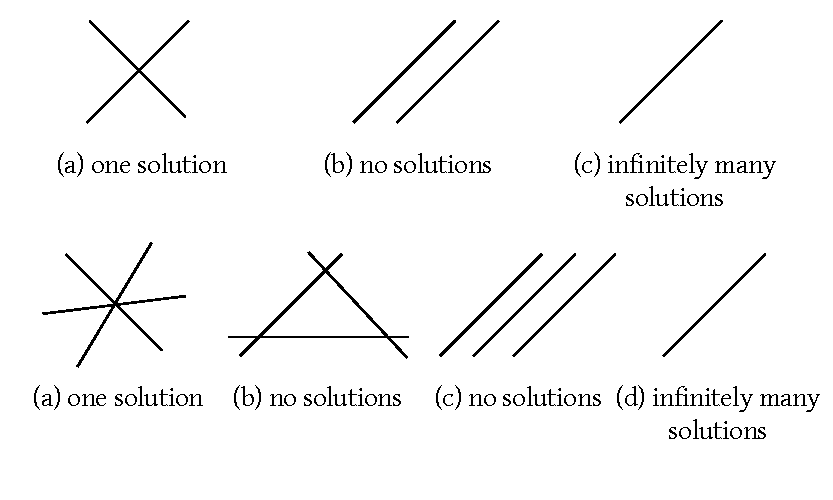
\includegraphics[width=0.5\textwidth]{img/linear_equation_visualization.pdf}
    \caption{
      Depiction of solutions of a linear equation system
      (with $m=2$ and $n=2$ in the upper row and $m>2$ and $n=2$ in the lower row)
    }
    \label{img:lineqsys-solutions}
  \end{center}
\end{figure}

\begin{figure}[t]
  \begin{center}
    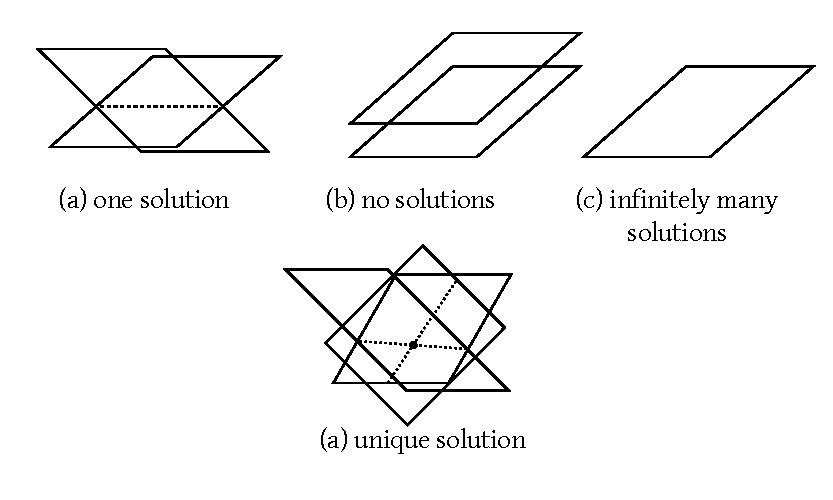
\includegraphics[width=0.5\textwidth]{img/linear_equation_visualization2.pdf}
    \caption{
      Depiction of solutions of a linear equation system
      (with $m=2$ and $n=3$ in the upper row and $m=3$ and $n=3$ in the lower row)
    }
    \label{img:lineqsys-solutions2}
  \end{center}
\end{figure}

\begin{description}
  \item[Case 4]
    A solution, where only two lines intersect. But not all three at one time.
  \item[Case 5]
    Two equations are equivalent, but other equations are parallel or intersecting.
\end{description}

What if there are 3 unknown variables, but only one equation?

\begin{description}
  \item[Case 6]
    No unique solution. Express one variable by others.
    Equation describes a layer.
\end{description}

What if there are three variables and two equations?

\begin{description}
  \item[Case 7] Two layers intersect in one line
  \item[Case 8] Two layers are parallel
\end{description}

What if there are three variables and three equations?

\begin{description}
  \item[Case 9] Intersection of three layers in one point
\end{description}

Or in general: point, line, layer, no solution or $\mathbb{R}^3$.
On a line we have one degree of freedom whereas $\mathbb{R}^3$ gives us three degrees of freeedom.

\paragraph{Example}
\begin{align*}
  -x  +y +2z &= 2 \\
  3x  -y  +z  &=6 \\
  -x +3y +4z &= 4
\end{align*}

We use Gauss-Jordan elimination:

\begin{align*}
  2 + 3\cdot 1 & 0\cdot 2y - 7z = 12 \\
  3 - 1        & 2y + 2z = 2
\end{align*}

The following equation system then has the same solution:

\begin{align*}
  -x + y + 2z &= 2 \\
  2y + 7z &= 12 \\
  2y + 2z &= 2
\end{align*}

We again use Gauss-Jordan elimination:

\begin{align*}
  2 - 3 & 0 + 5z = 10
\end{align*}

Therefore we derived:
\[ -x + y + 2z = 2 \]
\[ 2y + 2z = 2 \]
\[ 5z = 10 \]

Then $z = 2$, $y = -1$ and $x = 1$ follows.

Different notation (to save time \& space, matrix notation):
\[
  \left(\begin{array}{ccc|c}
    -1 &  1 &  2 &  2 \\
     3 & -1 &  1 &  6 \\
    -1 &  3 &  4 &  4 \\
   \hline
     0 &  2 &  7 & 12 \\
     0 &  2 &  2 &  2 \\
   \hline
       &  0 &  5 & 10
  \end{array}\right)
\] \[
  \left(\begin{array}{ccc|c}
    -1 &  1 &  2 & 2 \\
     0 &  2 &  2 & 2 \\
     0 &  0 &  5 & 10 \\
   \hline
    -1 &  1 &  2 & 2 \\
     0 &  1 &  1 & 1 \\
     0 &  0 &  1 & 2
  \end{array}\right)
\] \[
  \left(\begin{array}{ccc|c}
    -1 &  1 &  0 & -2 \\
     0 &  1 &  0 & -1 \\
     0 &  0 &  1 & 2 \\
   \hline
    -1 &  0 &  0 & -1 \\
     0 &  1 &  0 & -1 \\
     0 &  0 &  1 & 2 \\
   \hline
    -x &  0 &  0 & -1 \\
     0 &  y &  0 & -1 \\
     0 &  0 &  z & 2
  \end{array}\right)
\]

Distinct solution.

\paragraph{Another example:}

\begin{align*}
  x + y + z &= 1 \\
  x - 2z + 2z &= 2 \\
  4x + y + 3z &= 5
\end{align*}

\[
  \left(\begin{array}{ccc|c}
     1 &  1 &  1 & 1 \\
     1 & -2 &  2 & 2 \\
     4 &  1 &  5 & 5 \\
   \hline
     0 & -3 &  1 & 1 \\
     0 & -3 &  1 & 1 \\
   \hline
     0 &  0 &  0 & 0
  \end{array}\right)
\]

We encountered a tautology $0 = 0$. We have two pivot rows left:

\[
  \left(\begin{array}{ccc|c}
     1 &  1 &  1 & 1 \\
     0 & -3 &  1 & 1 \\
   \hline
     1 &  4 &  0 & 0 \\
     0 & -3 &  1 & 1 \\
   \hline
     x & +4y &    &= 0 \\
     0 & -3y & +z &= 1
  \end{array}\right)
\]

$y$ can be chosen arbitrarily. $y = t$ once $y$ has been defined.
\[ z = 1 + 3y = 1 + 3t \]
\[ x = -4y = -4t \]

The solution set is given as:
\[ \setdef{(-4t, t, 1 + 3t)}{t \in \mathbb{R}} \]

This represents a line in $\mathbb{R}^3$.

\paragraph{Example without solution}
\begin{align*}
  3x + 2y + z & =3 \\
  2x +  y + z &= 0 \\
  6x + 2y + z &= 6
\end{align*}

\[
  \left(\begin{array}{ccc|c}
      3 &  2 &  1 & 3 \\
      2 &  1 &  1 & 0 \\
      6 &  2 &  4 & 6 \\
   \hline
     -1 & -1 &  0 & -3 \\
     -6 & -6 &  0 & -6 \\
   \hline
     0 &   0 &  0 & 12
  \end{array}\right)
\]

There is no solution to $0 = 12$. Therefore no solution is possible for the equation system.

\subsection{Gauss-Jordan elimination algorithm}

\begin{enumerate}
  \item Write matrix
  \item Find $a_{ij} \neq 0$ (\enquote{pivot element} which was not a pivot element before, $i$-th row = pivot row, $j$-th row = pivot column)
    \begin{enumerate}
      \item mark $a_{ij}$
      \item subtract $\frac{a_{kj}}{a_{ij}}$ times i-th row from the k-th row for every $k \neq i$.
        In the j-th row a zero is created.
    \end{enumerate}
  \item If no new pivot element can be found:
    \begin{enumerate}
      \item Delete all rows, which only have 0s on the left and right side
      \item If there is a row which contains only 0s on the left side
        \begin{enumerate}
          \item If right-hand side is not 0, \textsc{No Solution!}
          \item If right-hand side is 0, apply back substitution meaning
          \item Iterate over all pivot elements in reversed order and create 0 in corresponding pivot column
          \item All columns which look like the pivot column, are assigned to free parameters
          \item those $x_j$, which are assigned to pivot columns, can be represented by the right side and free parameters
        \end{enumerate}
    \end{enumerate}
\end{enumerate}

\paragraph{Example with 4 equations}
\label{sec:1-4-6}

\[
  \left(\begin{array}{cccc|c}
     1 &  2 &  3 &  4 &  5 \\
     1 &  0 &  1 & -2 & -3 \\
     2 &  3 &  4 &  5 &  6 \\
     1 &  1 &  1 &  1 &  1 \\
   \hline
     0 & -2 & -2 & -6 & -8 \\
     0 & -1 & -2 & -3 & -4 \\
     0 & -1 & -2 & -3 & -4 \\
  \end{array}\right)
\]

First row is pivot row. First column is pivot column.
2nd row and 2nd column have not been pivot elements yet.

\[
  \left(\begin{array}{cccc|c}
    0 &  0 &  2 &  0 &  0
  \end{array}\right)
\]

Therefore $2x_3 = 0$.

\[
  \left(\begin{array}{cccc|c}
     0 &  0 &  0 &  0 &  0
  \end{array}\right)
\]

We have found an equivalent system:

\[
  \left(\begin{array}{cccc|c}
     1 &  2 &  3 &  4 &  5 \\
     0 & -1 & -2 & -3 & -4 \\
     0 &  0 &  2 &  0 &  0 \\
  \end{array}\right)
\]

$4$ is a free parameter. Therefore we set $x_4 = t$.
From $2x_3 = 0$, $x_3 = 0$ follows.

\[
  \left(\begin{array}{cccc|c}
     1 &  2 &  0 &  4 &  5 \\
     0 & -1 &  0 & -3 & -4 \\
     0 &  0 &  1 &  0 &  0 \\
   \hline
     1 &  0 &  0 & -2 & -3 \\
     0 & -1 &  0 & -3 & -4 \\
     0 &  0 &  1 &  0 &  0
  \end{array}\right)
\]

\begin{align*}
  x_4 &= t \\
  x_3 &= 0 \\
  -x_2 - 3x_4 &= -4 \\
  x_2 = 4 - 3x_4 &= 4 - 3t \\
  x_1 - 2x_4 &= -3 \\
  x_1 = -3 + 2x_4 &= -3 + 2t
\end{align*}

Solution set: $\setdef{(-3 + 2t, 4 - 3t, 0, t)}{t \in \mathbb{R}}$

\section{Vector spaces}

A vector is an element of $\mathbb{R}^n$ ($\mathbb{R}^n = \mathbb{R} \times \mathbb{R} \times \ldots \times \mathbb{R}$):
\[ \setdef{\begin{pmatrix} a_1 \\ a_2 \\ \vdots \\ a_n\end{pmatrix}}{a_i \in \mathbb{R}} \]
Column vectors or n-tuples in $\mathbb{R}^n$.

We define addition:
\[
  \begin{pmatrix} a_1 \\ a_2 \\ \vdots \\ a_n \end{pmatrix} +
  \begin{pmatrix} b_1 \\ b_2 \\ \vdots \\ b_n \end{pmatrix} \coloneqq
  \begin{pmatrix} a_1 + b_1 \\ a_2 + b_2 \\ \vdots \\ a_n + b_n \end{pmatrix}
\]

Multiplication for $\lambda \in \mathbb{R}$:
\[
    \lambda \cdot \begin{pmatrix} a_1 \\ a_2 \\ \vdots \\ a_n \end{pmatrix} \coloneqq
    \begin{pmatrix} \lambda a_1 \\ \lambda a_2 \\ \vdots \\ \lambda a_n \end{pmatrix}
\]

Geometric interpretation for $n=1,2,3,\ldots$:
  For $n \leq 3$ we can think of $n$-tuples as points on lines, layers or within the room.

Let $S$ be the set of all pairs of points ($A, B$). Consider it as directed path from $A$ to $B$.
Equivalence relation on $S$:
\[ (A, B) \sim (A', B') \]
if $(A', B')$ comes from $(A, B)$ using a parallel translation.

Is parallel translation an equivalence relation?
\begin{description}
  \item[reflexivity]
    $(A, B) \sim (A, B)$, \checkmark
  \item[symmetry]
    if $(A, B) \sim (A', B')$ then also $(A', B') \sim (A, B)$,
    inversed parallel translation,
    \checkmark
  \item[transitivity]
    if $(A, B) \sim (A', B')$ and $(A', B') \sim (A'', B'')$, then $(A, B) \sim (A'', B'')$,
    composition of parallel translations, \checkmark
\end{description}

A vector is therefore an equivalence class of directed paths.

\[ \overrightarrow{PQ} = [(P, Q)] \]

The set of vectors is in bijection with the set of points.
In every equivalence class there is one representative of structure $(0, A)$.
$\overrightarrow{0A}$ is called position vector (dt. Ortsvektor) to $A$.

\paragraph{Vector operations}
\begin{figure}[!h]
  \begin{center}
    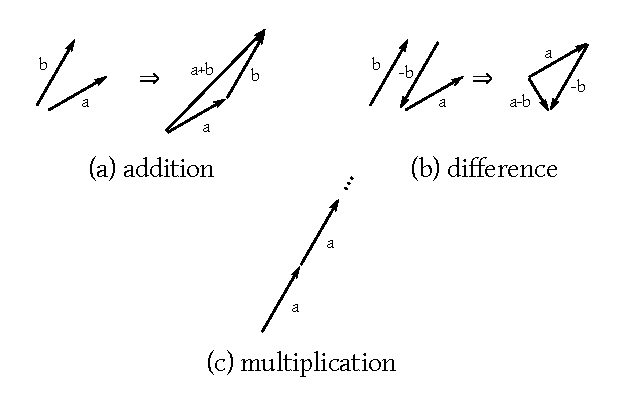
\includegraphics[width=0.5\textwidth]{img/vector_operations.pdf}
    \caption{Vector operations}
    \label{img:vector-operations}
  \end{center}
\end{figure}

Compare with Figure~\ref{img:vector-operations}.

\subsection{Properties}

\subsubsection{Addition}

Commutativity law:
\[ a + b = b + a \]

Associativity law:
\[ a + (b + c) = (a + b) + c \]

Zero vector:
\[ a + -a = 0 \]

\subsubsection{Multiplication}

Associativity law:
\[ \lambda \cdot (\mu \cdot a) = (\lambda \cdot \mu) \cdot a \]

Distributivity law:
\[ (\lambda + \mu) \cdot a = \lambda a + \mu a \]
\[ \mu \cdot (a + b) = \lambda a + \lambda b \]

\subsection{Applications}
\subsubsection{Diagonals of a parallelogram}
%
\begin{figure}[!h]
  \begin{center}
    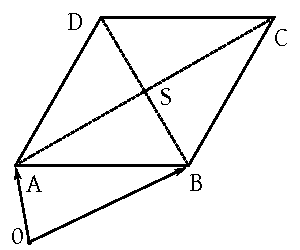
\includegraphics[width=0.2\textwidth]{img/parallelogram.pdf}
    \caption{Parallelogram and intersection $S$ of diagonals}
    \label{img:parallelogram}
  \end{center}
\end{figure}

The diagonals of a parallelogram intersect exactly on the halfway of the whole diagonal (compare with Figure~\ref{img:parallelogram}).
Hence we claim $\card{AS} = \card{SC}$ and $\card{BS} = \card{SD}$.
Let $M$ be the midpoint of $\overline{AC}$ and $N$ be the midpoint of $\overline{BD}$.
Then $M = N$ must hold.

Let's assume the opposite ($M \neq N$).
\[ \overrightarrow{CM} = \overrightarrow{OA} + \frac12 \overrightarrow{AC} \]
\[ = \overrightarrow{0A} - \frac12 \left(\overrightarrow{AB} + \overrightarrow{BC}\right) \]
\begin{align*}
  \overrightarrow{0N} &= \overrightarrow{0B} + \frac12 \overrightarrow{BD} \\
    &= \overrightarrow{0A} + \overrightarrow{AB} + \frac12 \overrightarrow{BD} \\
    &= \overrightarrow{0A} + \overrightarrow{AB} + \frac12 \left(\overrightarrow{BC} + \overrightarrow{CD}\right) \\
    &= \overrightarrow{0A} + \overrightarrow{AB} + \frac12 \left(\overrightarrow{AD} + \overrightarrow{BA}\right) \\
    &= \overrightarrow{0A} + \overrightarrow{AB} + \frac12 \overrightarrow{AD} - \frac12 \overrightarrow{AB} \\
    &= \overrightarrow{0A} + \frac12 \overrightarrow{AB} + \frac12 \overrightarrow{AD} \\
    &= \overrightarrow{0M}
\end{align*}

\subsubsection{Line crossing two points}
%
\begin{figure}[!h]
  \begin{center}
    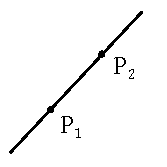
\includegraphics[width=0.2\textwidth]{img/line_with_P1_and_P2.pdf}
    \caption{Lines with $P_1$ and $P_2$}
    \label{img:line}
  \end{center}
\end{figure}
%
The line crossing two points $P_1$ and $P_2$ (see Figure~\ref{img:line}) is defined as
\[ \setdef{\overrightarrow{0P_1} + t \cdot \overrightarrow{P_1 P_2}}{t \in \mathbb{R}} \]
\[ = \setdef{\overrightarrow{0P_1} + t \cdot \left(\overrightarrow{0P_2} - \overrightarrow{0P_1}\right)}{t \in \mathbb{R}} \]

\subsubsection{A layer can be defined by three points}

A layer can be defined by three points $P_1$, $P_2$ and $P_3$.

\[ \setdef{\overrightarrow{0P_1} + s \cdot \overrightarrow{P_1 P_2} + t \cdot \overrightarrow{P_1 P_3}}{s, t \in \mathbb{R}} \]

\subsection{Algebraic structures}

A set $M$ with a mapping $\circ: M \times M \rightarrow M$ ($(x, y) \mapsto x \circ y$)
is called \emph{Magma} or \emph{algebraic structure}.

\subsubsection{Examples}

Examples for $M$:

\[ \mathbb{N}, \mathbb{Q}, \mathbb{R}, \mathbb{Z}, \mathbb{C} \]

Examples for mappings $\circ$:

\[ \circ = +, \cdot \]
\[ x \circ y = x + y \]
\[ x \circ y = x \cdot y \]

\begin{enumerate}
  \item Example $M = \mathbb{N}$ and $x \circ y = x^y$.
  \item Example $M = \set{\pm 1}$ and $x \circ t = x \cdot y$.

    \begin{table}[!ht]
      \begin{center}
        \begin{tabular}{c|cc}
         & +1 & -1 \\
        \hline
          +1 & +1 & -1 \\
          -1 & -1 & +1
        \end{tabular}
        \caption{composition table}
      \end{center}
    \end{table}

  \item Example $M = \mathcal{P}(X)$ and
    \[
      A \circ B =
      \begin{cases}
        A \cap B \\
        A \cup B \\
        A \triangle B
      \end{cases}
    \]

  \item Example $M = \set{a, b, c, e}$ and

    \begin{table}[!ht]
      \begin{center}
        \begin{tabular}{c|cccc}
            & a & b & c & e \\
         \hline
          a & e & c & b & a \\
          b & c & e & a & b \\
          c & b & a & e & c \\
          e & a & b & c & e \\
        \end{tabular}
        \caption{composition table}
      \end{center}
    \end{table}

  \item
    Example $A = \set{a, b, c, \dots}$ where the set is the alphabet.
    Then $M = \setdef{a_1, \ldots, a_n}{n \in \mathbb{N}, a_i \in A}$ is the set of words.
    Then our composition is defined as
    \[ a_1 \ldots a_m \circ b_1 \ldots b_n = a_1 \ldots a_m b_1 \cdot b_n \]
    $A^*$ is the set of possible words.
    $A^+$ is defined as $A^* \setminus \set{\varepsilon}$ where $\varepsilon$ is the empty word.

  \item
    Example $M = X^X = \set{f: X \rightarrow X}$ of an arbitrary set. $f \circ g$ is the composition (compute $f$ after $g$).
\end{enumerate}

\subsection{Compositions}

Let $(M, a)$ be a Magma. The composition is called

\begin{description}
  \item[associative if]
    \[ \bigwedge_{x,y,z \in M} (x \circ y) \circ z = x \circ (y \circ z) \]
  \item[commutative if]
    \[ \bigwedge_{x,y \in M} x \circ y = y \circ x \]
\end{description}

All examples above are associative\footnote{Assuming the first example uses addition. $x^y$ is not associative.}.
The last two examples are not commutative; others are\footnote{Assuming the first example uses addition. $x^y$ is not commutative.}

An element $e \in M$ is called
\begin{description}
  \item[left-neutral if] \[ \bigwedge_{x \in M} e \circ x = x \]
  \item[right-neutral if] \[ \bigwedge_{x \in M} x \circ e = x \]
\end{description}
A neutral element is left- and right-neutral.

Applied to the examples:
\begin{enumerate}
  \item $0$ acts as neutral element in addition. $1$ is the neutral element of multiplication.
  \item $1$ is the neutral element
  \item $A \cap B$ ($X$ as neutral element), $A \cup B$ ($\emptyset$ as neutral element), $A \triangle B$ is left for the practicals
  \item $e$ as neutral element
  \item $\varepsilon$ as neutral element
  \item identity function acts as neutral element, $\operatorname{id} \circ f = f' = f \circ \operatorname{id}$
\end{enumerate}

Let $(M, \circ)$ be a magna with a neutral element $e$.
Let $x \in M$, then $y \in M$ is called
\begin{description}
  \item[left-inverse if] $y \circ x = e$
  \item[right-inverse if] $x \circ y = e$
\end{description}
An \emph{inverse} element to $x$ is left- and right-inverse simultaneously.
$x$ is \emph{invertible} if an inverse element exists.

Applied to examples:
\begin{enumerate}
  \item
    $(\mathbb{N}_0, +)$ has no inverse element.
    $(\mathbb{Z}, +)$ has an inverse element to $x$: $-x$.
    Same for $\mathbb{Q}$ and $\mathbb{R}$.
    $(\mathbb{N}, \cdot)$ has inverse element $\set{1}$.
    All non-zero elements in $(\mathbb{Q}, \cdot)$ are invertible.

  \item
    $(\mathbb{Z}, \cdot)$ has inverse elements $\set{\pm 1}$.

  \item
    $A \cap B = X$: inverse elements are $\set{X}$.
    $A \cup B = \emptyset$: inverse elements are $\set{\emptyset}$
    $A \triangle B$ is left as an exercise.

  \item
    All elements are invertible to themselves

  \item
    For $a_1, \ldots, a_m$, the invertible elements are $\set{\varepsilon}$

  \item
    The invertible elements are defined by any bijective mapping $X \rightarrow X$.
\end{enumerate}

A \emph{semigroup} is a magma with associative composition.
A \emph{monoid} is a semigroup with a neutral element.
A group is a monoid where every element is invertible.
An \emph{abelian group} (or commutative group) is a semigroup, monoid or group with a commutative composition.

\fbox{Niels Henrik Abel (1802--1829)}

Examples:
\begin{enumerate}
  \item $(\mathbb{N}, +)$ is a semi-group.
        $(\mathbb{N}_0, +)$ is a monoid.
        $(\mathbb{N}, \cdot)$ is a monoid.
        $(\mathbb{Z}, +)$ is a group.
        $(\mathbb{Z}, \cdot)$ is a monoid.
        $(\mathbb{Q} \setminus \set{0}, \cdot)$ is a group.
        $(\mathbb{R} \setminus \set{0}, \cdot)$ and $(\mathbb{C} \setminus \set{0}, \cdot)$ are also groups.
        All of them are abelian.
  \item is a group and abelian.
  \item $(\mathcal{P}(X), \cap)$ and $(\mathcal{P}(X), \cup)$ are monoids. $(\mathcal{P}(X), \triangle)$ is an abelian group.
  \item is an abelian group
  \item $(A^+, \cdot$ is a semi-group (non-commutative). $(A^*, \circ$ is a monoid (non-commutative).
        \[ \mathbb{N} = A^t \text{ where } A = \set{a} \]
  \item $(X^X, \circ)$ is a non-commutative monoid
\end{enumerate}

\begin{theorem}
  A magma ($G, \circ$) is a group iff
  \begin{description}
    \item[G1] $\bigwedge_{x,y,z} (x \circ y) \circ z = x \circ (y \circ z) \hspace{20pt} \text{\enquote{associative}}$
    \item[G2] $\bigvee_{e \in G} \bigwedge_{x} e \circ x = x \hspace{20pt} \text{\enquote{left-neutral element}}$
    \item[G3] $\bigwedge_x \bigvee_y y \circ x = e \hspace{20pt} \text{\enquote{left-inverse element}}$
  \end{description}
  Neutral elements are necessarily right-neutral / right-inverse.
\end{theorem}

\begin{proof}
  Show that
  \begin{itemize}
    \item[i.] any left-neutral element is right-neutral
    \item[ii.] left-inverse elements are right-inverse
  \end{itemize}

  \begin{itemize}
    \item[ii.]  Let $x, y \in G$. $y$ is left-inverse to $x$: $y \circ x = e$.
      Show that $x \circ y = e$.
      \[ x \circ y = e \circ (x \circ y) = (z \circ y) \circ (x \circ y) \]
      From G3 it follows that
      \[ \bigvee_{z} z \circ y = e \]
      From associativity it follows that $z \circ (y \circ x) \circ y \Rightarrow z \circ (e \circ z) \Rightarrow z \circ y = e$.
    \item[i.]
      Let $x, y \in G$ with inverse elements $x^{-1}$ and $y^{-1}$.
      Let $z = y^{-1} \circ x^{-1}$. Then,
      \begin{align*}
        (x \circ y) \circ z &= (x \circ y) \circ (y^{-1} \circ x^{-1}) \\
          &= x \circ \underbrace{y \circ y^{-1}}_{e} \circ x^{-1} \\
          &= x \circ e \circ x^{-1} \\
          &= x \circ x^{-1} \\
          &= e
      \end{align*}
      So $x \circ y$ is right-invertible (analogously left-invertible)
      \[ \Rightarrow x \circ y \in G \]

      %Let $x \in G$. Show that $x \circ e = x$.

      %Let $y$ be a left-inverse of $x$
      %\[ \Rightarrow z \circ x = e \Rightarrow x \circ e = x \circ (z \circ x) \]
      %\[ \Rightarrow (x \circ z) \circ x \Rightarrow e \circ x \Rightarrow x \]
  \end{itemize}
\end{proof}

\begin{theorem}
  \label{satz-2-10}
  Let $(G, \cdot)$ be a group.
  \begin{enumerate}
    \item The neutral element is unique
    \item Inverse elements are unique (therefore every element has exactly one inverse)
    \item Equivalence laws:
      \[ \bigwedge_{x,y,z \in G} x \circ z = y \circ z \implies x = z \]
      \[ \bigwedge_{x,y,z \in G} z \circ x = z \circ y \implies x = y \]
  \end{enumerate}
\end{theorem}

\begin{proof}
  \begin{enumerate}
    \item Let $e'$ be another neutral element:
      \[ e' \underbrace{=}_{e \text{ is neutral}} e' \circ e \underbrace{=}_{e' \text{ is neutral}} e \]
    \item Let $y, y'$ be two inverse elements to $x$
      \[ y \circ x = e = x \circ y \]
      \[ y' \circ x = e = x \circ y' \]
      Show that $y = y'$:
      \[ y = y \circ e = y \circ (x \circ y') = (y \circ x) \circ y' = e \circ y' = y' \]
    \item Let $x \circ z = y \circ z$. Let $w$ be inverse to $z$: $z \circ w = e$.
      \[ (x \circ z) \circ w = (y \circ z) \circ w \]
      \[ x \circ (z \circ w) = y \circ (z \circ w) \]
      \[ x \circ e = y \circ e \]
      \[ x = y \]
  \end{enumerate}
\end{proof}

\begin{itemize}
  \item The unique inverse element of Theorem~\ref{satz-2-10} (2) of $x$ is denoted with $x^{-1}$.
  \item
    Abelian groups are typically written additive.
    In $(G, +)$ the inverse element is denoted $-x$.
\end{itemize}

\begin{theorem}
  \label{satz-2-12}
  Let $(M, \cdot)$ be a monoid. Then $\setdef{x \in M}{x \text{ is invertible}}$ is a group.
\end{theorem}

\begin{proof}
  Let $G = \setdef{x \in M}{x \text{ is invertible}}$.
  Show that
  \begin{enumerate}
    \item If $x, y \in G$, then also $x \circ y \in G$.
    \item Associativity is inherited from $M$.
    \item A neutral element $e \in G$ exists.
    \item All elements are invertible in $G$.
  \end{enumerate}

  Proof:
  \begin{enumerate}
    \item Let $x, y \in G$ with inverse $x^{-1}, y^{-1}$.
      Let $z = y^{-1} \circ x^{-1}$.
      Then it holds that
      \begin{align*}
        (x \circ y) \circ z &= (x \circ y) \circ (y^{-1} \circ x^{-1}) \\
          &= x \circ y \circ y^{-1} \circ x^{-1} \\
          &= x \circ e \circ x^{-1} \\
          &= x \circ x^{-1} \\
          &= e
      \end{align*}
      \[ x \circ y \text{ is right invertible (analogously: left invertible)} \]
      \[ \Rightarrow x \circ y \in G \]
    \item follows immediately
    \item $e \circ e = e \implies e \text{ is invertible} \implies e \in G$
    \item $x \in G \implies x^{-1} \in G$ because $x^{-1} \circ x = e \implies (x^{-1})^{-1} = x$
  \end{enumerate}
\end{proof}

\meta{lecture}{27th of Oct 2015}{Prof. Franz Lehner}

\begin{table}
  \begin{center}
    \begin{tabular}{ll}
     \hline
      Magma & $(M, \circ)$, $\circ: M \times M \rightarrow M$ \\
      Semigroup & +associative \\
      Monoid & +neutral element $e$: $e \circ a = a = a \circ e$ \\
      Group & invertibility of all elements: $\bigwedge_x \bigvee_y x\circ y = e = y \circ x$ \\
     \hline
    \end{tabular}
    \caption{Group theory cheatsheet}
  \end{center}
\end{table}

\begin{theorem}
  \label{satz-2-9}
  Let $(M,\circ)$ be a group.
  \begin{align*}
    \stackrel{G1}{\Rightarrow} & \text{ associative } \\
    \stackrel{G2}{\Rightarrow} & \bigvee_e \bigwedge_x e \circ x = x \\
    \stackrel{G3}{\Rightarrow} & \bigvee_x \bigwedge_y y \circ x = e
  \end{align*}

  Show that
  \begin{itemize}
      \item[i.] A left-neutral element is right-neutral
      \item[ii.] Left-inverse elements are also right-inverse
  \end{itemize}
\end{theorem}

\begin{proof}
  \begin{itemize}
    \item[ii.]
      Let $x \in G \stackrel{G3}{\Rightarrow} \bigvee_y y \circ x = e$.
      Show that $x \circ y = e$.
      \begin{align*}
        x \circ y \stackrel{G2}{=} e \circ (x \circ y) &= (z \circ y) \circ (x \circ y) \\
        \stackrel{G3}{\Rightarrow} \bigvee_{z} z \circ y = e \\
        &\stackrel{G1}{=} z \circ (y \circ x) \circ y \\
        &= z \circ (e \circ y) \\
        &= z \circ y = e
      \end{align*}
    \item[i.]
      Let $x \in G$, show that $x \circ e = x$. Let $y$ be left-inverse to $x$.
      $e = y \circ x$.
      \[ x \circ e = x \circ (y \circ x) \stackrel{G1}{=} (x \circ y) \circ x = e \circ x \stackrel{G2}{=} x \]
      \[ \Rightarrow e \text{ is also right-neutral} \]
  \end{itemize}
\end{proof}

How do we construct groups? We select an associative $(M, \circ)$.
$G = \setdef{x \in M}{x \text{ invertible}}$ is a group.

\begin{cor}
  \[ (M, \circ) = (X^X, \circ) = \set{f: X \rightarrow X} \]
  \[ S_X = \set{f: X \rightarrow X \text{ bijective}} \]
  $(S_X, \circ)$ is a group ($\circ$ is composition of functions)
  and is called \emph{symmetric group} over $X$ or \emph{permutation group} (if $\card{X} < \infty$).
\end{cor}

\begin{cor}
  Let $X = \set{1, \ldots, n}$. Let $\pi: \set{1, \ldots, n} \rightarrow \set{1, \ldots, n}$ bijective.
  Then $\pi$ is typically written as scheme
  \[
    \begin{pmatrix}
       1 & 2 & \ldots & n \\
       \vdots & \vdots & \ddots & \vdots \\
       \pi(1) & \pi(2) & \ldots & \pi(n)
    \end{pmatrix}
  \]
  is called \emph{permutation} (rearrangement).

  For finite sets $f: \set{1, \ldots, n} \rightarrow \set{1, \ldots, n}$ is bijective.
  $\Leftrightarrow$ $f$ is injective. $\Leftrightarrow$ $f$ is surjective.
  This does not hold for infinite sets.
  \[ f: \mathbb{N} \rightarrow \mathbb{N} \]
  \[ f(n) = 2n \]
  is injective, but not surjective
\end{cor}

\[
  S_2
    = S_{\set{1,2}}
    = \set{\begin{pmatrix} 1 & 2 \\ 1 & 2 \end{pmatrix}, \begin{pmatrix} 1 & 2 \\ 2 & 1 \end{pmatrix}}
\] \[
  =
  \set{\begin{array}{ccc} 1 & \mapsto & 2 \\ 1 & \mapsto & 2 \end{array}, \begin{array}{ccc} 1 & \mapsto & 2 \\ 2 & \mapsto & 1 \end{array}}
\] \[
  S_3
    = S_{\set{1,2,3}}
    = \set{
      \begin{pmatrix} 1 & 2 & 3 \\ 1 & 2 & 3 \end{pmatrix},
      \begin{pmatrix} 1 & 2 & 3 \\ 1 & 3 & 2 \end{pmatrix},
      \begin{pmatrix} 1 & 2 & 3 \\ 2 & 1 & 3 \end{pmatrix},
      \begin{pmatrix} 1 & 2 & 3 \\ 2 & 3 & 1 \end{pmatrix},
      \begin{pmatrix} 1 & 2 & 3 \\ 3 & 2 & 1 \end{pmatrix},
    }
\] \[
  \card{S_n} = n!
\]

$S_3$ is non-commutative!
\[ \neg \bigwedge_{\pi, \phi \in S_3} \pi \circ \varphi = \varphi \circ \pi \]

\begin{ex}
  \[
    \begin{pmatrix} 1 & 2 & 3 \\ 2 & 1 & 3 \end{pmatrix}
    \hspace{10pt}
    \begin{pmatrix} 1 & 2 & 3 \\ 1 & 3 & 2 \end{pmatrix}
  \]
  \[
    \begin{pmatrix} 1 & 2 & 3 \\ 2 & 1 & 3 \end{pmatrix}
      \circ \begin{pmatrix} 1 & 2 & 3 \\ 1 & 3 & 2 \end{pmatrix}
      = \begin{pmatrix} 1 & 2 & 3 \\ 2 & 3 & 1 \end{pmatrix}
      \neq \begin{pmatrix} 1 & 2 & 3 \\ 1 & 3 & 2 \end{pmatrix}
      \circ \begin{pmatrix} 1 & 2 & 3 \\ 2 & 1 & 3 \end{pmatrix}
      = \begin{pmatrix} 1 & 2 & 3 \\ 3 & 1 & 2 \end{pmatrix}
  \]
\end{ex}

\begin{ex}
  \label{bsp-2-14}
  Symmetry group of a rectangle:
  The group of motions, which keeps the rectangle invariant
  (ie. the rectangle is mapped to itself)
  \begin{itemize}
    \item \emph{not} translation
    \item rotation
    \item mirroring
  \end{itemize}

  Horizontal mirroring:
  \[
    h \stackrel{\sim}{=}
    \begin{pmatrix}
      A & B & C & D \\
      D & C & B & A
    \end{pmatrix}
  \]

  Vertical mirroring:
  \[
    V \stackrel\sim=
    \begin{pmatrix}
      A & B & C & D \\
      B & A & D & C
    \end{pmatrix}
  \]
  \[
    d_\pi \stackrel\sim=
    \begin{pmatrix}
      A & B & C & D \\
      C & D & A & B
    \end{pmatrix}
  \]

  Notes to create composition table:
  \[
    v \circ h =
    \begin{pmatrix}
      A & B & C & D \\
      D & C & B & A \\
      C & D & A & B
    \end{pmatrix}
    = \begin{pmatrix}
      A & B & C & D \\
      C & D & A & B
    \end{pmatrix}
    = d_\pi
  \]
  \[ (v \circ h)^{-1} = d_\pi^{-1} = d_\pi \]
  \[ h^{-1} \circ v^{-1} = h \circ v \]
  \[ h \circ d_\pi = h\circ (h\circ v) = (h \circ h) \circ v = \text{id} \circ v = v \]

  \begin{table}[!ht]
    \begin{center}
      \begin{tabular}{c|cccc}
       \hline \hline
        $\circ     $ & $\text{id} $ & $h        $ & $v        $ & $d_\pi    $ \\
       \hline
        $\text{id} $ & $\text{id} $ & $h        $ & $v        $ & $d_\pi    $ \\
        $h         $ & $h         $ & $\text{id}$ & $d_\pi    $ & $v        $ \\
        $v         $ & $v         $ & $d_\pi    $ & $\text{id}$ & $h        $ \\
        $d_\pi     $ & $d_\pi     $ & $v        $ & $h        $ & $\text{id}$ \\
       \hline \hline
      \end{tabular}
      \caption{
        Composition table for symmetry group of rectangles.
        The diagonal $\text{id}$ represents that all elements are inverse to themselves.
        This table is symmetrical. Therefore this group is commutative.
      }
    \end{center}
  \end{table}
\end{ex}

\begin{theorem}
  \label{2.15}
  Computations modulo $n$. The relation
  \[ x \equiv y \mod{n} \Leftrightarrow \divides{n}{x - y} \]
  is an equivalence relation on $\mathbb{Z}$.
  The equivalence classes
  \[ [x]_n = \setdef{x + q \circ n}{q \in \mathbb{Z}} \]
  are called \emph{residuo modulo classes} or \emph{congruence classes modulo n}.

  A system of representatives is
  \[ \set{0, \ldots, n-1} \]
  Factor set:
  \[ \mathbb{Z}_n := \mathbb{Z}/n = \mathbb{Z}/n\mathbb{Z} := \mathbb{Z}/\equiv_n \]
  We define addition and multiplication
  \[ [x]_n + [y]_n := [x + y]_n \]
  \[ [x]_n \cdot [y]_n := [x \cdot y]_n \]
\end{theorem}

Are we allowed to define it like that?
What about $[x]_n = [x + n]_n$?
Does the definition not depend on the definition of the system of representatives?

\begin{theorem}
  \label{Satz-2.16}
  \begin{itemize}
    \item[(i)] The addition on $\mathbb{Z}_n$ is well-defined if
      \[ x \equiv x' \mod{n} \qquad \text{(ie. $[x]_n = [x']_n)$} \]
      and
      \[ y \equiv y' \mod{n} \qquad \text{(ie. $[y]_n = [y']_n)$} \]
      then also $x + y \equiv x' + y' \mod{n}$ (ie. $[x+y]_n = [x' + y']_n$).

      $(\mathbb{Z}_n, +)$ is an abelian group with neutral element $[0]_n$
      and inverse elements $-[x]_n = [-x]_n$.
    \item[(ii)] The multiplication on $\mathbb{Z}_n$ is well-defined if
      \[ x \equiv x' \mod{n} \]
      and
      \[ y \equiv y' \mod{n} \]
      then also $x \circ y \equiv x' \cdot y' \mod{n}$ (ie. $[x\cdot y]_n = [x'\cdot y']_n$).
      $(\mathbb{Z}_n, \cdot)$ is a commutative matroid with neutral element $[1]_n$.
      $\mathbb{Z}_n^* = \mathbb{Z}_n \setminus \set{[0]_n}$ is a group if $n \in \mathbb{P}$
  \end{itemize}
\end{theorem}

\begin{proof}
  Let $x = x' \mod{n}$ and $y = y' \mod{n}$. Show that $x + y = x' + y'$ and $x\cdot y = x' \cdot y'$.
  $\divides{n}{x-x'}$ and $\divides{n}{y - y'}$. Show that
  \[ \divides{n}{(x+y) - (x' + y')} \text{ and } \divides{n}{x\cdot y - x'\cdot y'} \]

  So for addition,
  \[ \bigvee_k x - x' = k \cdot n \]
  \[ \bigvee_l y - y' = l \cdot n \]
  \begin{align*}
    \Rightarrow (x + y) - (x' - y')
      &= x + y - x' - y' \\
      &= x - x' + y - y' \\
      &= k \cdot n + l \cdot n \\
      &= (k + l) \cdot n \\
      &= \divides{n}{(x + y) - (x' + y')}
  \end{align*}

  For multiplication,
  \begin{align*}
    x \cdot y
      &= (x' + kn) \cdot (y' + ln) \\
      &= (x' \cdot y') + (k \cdot n \cdot y') + x' \cdot l \cdot n + k \cdot n \cdot l \cdot n \\
      &= x' \cdot y' + n (R\cdot y' + l \cdot x' + k \cdot l \cdot n)
  \end{align*}
  \[ xy - x' y' = \text{ multiple of } n \]
  \[ \Rightarrow \divides{n}{xy - x'y'} \]
\end{proof}

\begin{ex}
  $(\mathbb{Z}_n, +)$ is a group?
  \begin{itemize}
    \item We show G1:
      \[ \left([x]_n + [y]_n\right) + [z]_n \stackrel?= [x]_n + \left([y]_n + [z]_n\right) \]
      \[ [x+y]_n + [z]_n \stackrel?= [x]_n + \left[y + z\right]_n \]
      \[ \Rightarrow \left[(x + y) + z\right]_n = \left[x + (y + z)\right]_n \]
    \item We show G2, by definition of $[0]_n$ as neutral element
      \[ [x]_n + [0]_n = [x + 0]_n = [x]_n \]
    \item We show G3, by definition of $[-x]_n$ as neutral element
      \[ [x]_n + [-x]_n = [x - x]_n = [0]_n \]
      Analogously,
      \[ \left([x]_n \cdot [y]_n\right) \cdot [z]_n = [x]_n \left([y]_n \cdot [z]_n\right) \]
      \[ [x]_n \cdot [1]_n = [x1]_n = [x]_n \]
      Therefore $[1]_n$ is the neutral element for multiplication
  \end{itemize}

  What is the inverse for multiplication?
  It is immediate, that $[0]_n$ has no inverse for multiplication.
  \[ [0]_n \cdot [x]_n = [0]_n \neq [1]_n \]
  in $\mathbb{Z}_n\setminus \set{[0]_n}$?

  Case distinction:
  \begin{description}
    \item[$n \not\in \mathbb{P}$]
      \[ \Rightarrow \bigvee_{1 < n_1, n_2 < n} n = n_1 \cdot n_2 \]
      \[ [n_1]_n \cdot [n_2]_n = [n_1 \cdot n_2]_n = [n]_n = [0]_n \]
      \[ \Rightarrow [n_1]_n \text{ has not inverse element!} \]
      Assume
      \[ \bigvee_{[x]_n} [n_1]_n \cdot [x]_n = [1]_n \]
      \[ \Rightarrow [n_2] \cdot [n_1] \cdot [x]_n = [n_2]_n [1]_n \]
      \[ \Rightarrow [0]_n = [n_2]_n \]
      This is a contradiction. No inverse can exist.
    \item[$n \in \mathbb{P}$]
      Beforehand, for prime numbers $p$ it holds that
      \[ \divides{p}{ab} \Rightarrow \divides{p}{a} \lor \divides{p}{b} \]

      \begin{theorem}
        We claim that every $[x]_n \neq [0]_n$ has an inverse.
      \end{theorem}
      \begin{proof}
        \[ V_X = \set{[x], [2x], [3x], \ldots, [(n-1) x]} \text{ multiples of } [x]_n \]
        Then $[0]_n \not\in V_x$. Assume
        \[ \bigvee_k [k\cdot x]_n = [0]_x \]
        therefore
        \[ \bigvee_k k \cdot x \equiv 0 \mod{n} \]
        \[ \Rightarrow \divides{n}{kx} \]
        \[ \Rightarrow \divides{n}{k} \lor \divides{n}{x} \]
        \[ \Rightarrow \divides{n}{x} \]
        \[ \Rightarrow [x]_n \]
        \[ \Rightarrow [0]_n \]
        This is a contradiction.
      \end{proof}

      \begin{theorem}
        All entries of $V_X$ are different.
      \end{theorem}
      \begin{proof}
        Assume
        \[ \bigvee_{1 \leq k, l \leq n-1} [kx]_n = [lx]_n \]
        \[ [kx]_n - [lx]_n = [0]_n \]
        \[ [(k-l) x] = [0]_n \]
        \[ \Rightarrow (k-l) x \equiv 0 \mod{n} \]
        \[ \Rightarrow \divides{n}{(k-l)x} \]
        \[ \Rightarrow \divides{n}{k-l} \lor \divides{n}{x} \]
        The second condition cannot hold.
        \[ \Rightarrow k - l = 0 \]
        Requirement: $[x]_n \neq [0]_n$.
      \end{proof}

      \[ \Rightarrow \set{[x]_n, [2x]_n, \ldots, [(n-1)x]} \subseteq \set{[1], [2], \ldots, [n-1]} \]
      are all different.
      \[ \Rightarrow \bigvee_{k}: [kv]_n = [1]_n \]
      \[ \Rightarrow [k]_n = [x]_n^{-1} \]
      $k$ is constructed using the Euclidean algorithm.
  \end{description}
\end{ex}

\begin{ex}
  \begin{table}[!ht]
    \begin{center}
      \begin{tabular}{c|ccccc}
        $+$ & 0 & 1 & 2 & 3 & 4 \\
          0 & 0 & 1 & 2 & 3 & 4 \\
          1 & 1 & 2 & 3 & 4 & 0 \\
          2 & 2 & 3 & 4 & 0 & 1 \\
          3 & 3 & 4 & 0 & 1 & 2 \\
          4 & 4 & 0 & 1 & 2 & 3
      \end{tabular}
      \caption{Composition table for $(\mathbb{Z}_5, +)$}
    \end{center}
  \end{table}
  \begin{table}[!ht]
    \begin{center}
      \begin{tabular}{c|ccccc}
        $\cdot$ & 0 & 1 & 2 & 3 & 4 \\
              0 & 0 & 0 & 0 & 0 & 0 \\
              1 & 0 & 1 & 2 & 3 & 4 \\
              2 & 0 & 2 & 4 & 1 & 3 \\
              3 & 0 & 3 & 1 & 4 & 2 \\
              4 & 0 & 4 & 3 & 2 & 1
      \end{tabular}
      \caption{
        Composition table for $(\mathbb{Z}_5, \cdot)$.
        Every row is a permutation of the first row.
        Every row (except $0$) has a $1$ element is therefore invertible.
      }
    \end{center}
  \end{table}
  \begin{table}[!ht]
    \begin{center}
      \begin{tabular}{c|ccccc}
        $\cdot$ & 1 & 2 & 3 & 4 \\
              1 & 1 & 2 & 3 & 4 & 5 \\
              2 & 2 & 4 & 0 & 2 & 4 \\
              3 & 3 & 0 & 3 & 0 & 3 \\
              4 & 4 & 2 & 0 & 4 & 2 \\
              4 & 5 & 4 & 3 & 2 & 1
      \end{tabular}
      \caption{
        Composition table for $(\mathbb{Z}_6, \cdot)$.
        $1$ and $5$ have a $1$-element and is therefore invertible.
      }
    \end{center}
  \end{table}

  In general $[x]_n$ is invertible iff $\gcd{(x, n)} = 1$.

  \begin{table}[!ht]
    \begin{center}
      \begin{tabular}{c|ccccc}
        $+$ & 0 & 1 \\
          0 & 0 & 1 \\
          1 & 1 & 0
      \end{tabular}
      \caption{Composition table for $(\mathbb{Z}_2, +)$}
    \end{center}
  \end{table}
  \begin{table}[!ht]
    \begin{center}
      \begin{tabular}{c|ccccc}
        $\cdot$ & +1 & -1 \\
             +1 & +1 & -1 \\
             -1 & -1 & +1
      \end{tabular}
      \caption{Composition table for $(\set{\pm 1}, \cdot)$}
    \end{center}
  \end{table}

  \[ h: \mathbb{Z}_2 \rightarrow \set{\pm 1} \]
  \[ [0]_2 \rightarrow +1 \]
  \[ [1]_2 \rightarrow -2 \]
  The composition table of $\mathbb{Z}_2$ maps to composition table of $\set{\pm 1}$.

  Therefore
  \[ h([x] + [y]) = h([x]) \cdot h([y]) \forall [x], [y] \]
\end{ex}

\index[German]{\foreignlanguage{ngerman}{Homomorphismus}}
\index[English]{Homomorphism}
\index[German]{\foreignlanguage{ngerman}{Gruppenhomomorphismus}}
\index[English]{Group homomorphism}
\begin{defi}
  Let $(G_1, \circ)$ and $(G_2, \circ)$ be 2 groups. A map
  \[ h: G_1 \rightarrow G_2 \]
  is called group-homomorphism if it holds that
  $\bigwedge_{x,y \in G_1} h(x \circ_1 y) = h(x) \circ_2 h(y)$.
\end{defi}

\meta{lecture}{3rd of November 2015}{Franz Lehner}

\index[English]{Embedding}
\index[German]{\foreignlanguage{ngerman}{Einbettung}}
\index[English]{Field embedding}
\index[German]{\foreignlanguage{ngerman}{Epimorphismus}}
\index[English]{Epimorphism}
\index[German]{\foreignlanguage{ngerman}{Isomorphismus}}
\index[English]{Isomorphism}
\begin{defi}
  Let $(G_1, \circ_1)$ and $(G_2, \circ_2)$ be groups. A mapping $h: G_1 \rightarrow G_2$
  is called group-homomorphism if $h(a \circ_1 b) = h(a) \circ_2 h(b)$ for all $a, b \in G_1$.

  Additionally
  \begin{itemize}
    \item if $h$ is injective, the mapping is called \enquote{field embedding}.
    \item if $h$ is surjective, the mapping is called \enquote{epimorphism}.
    \item if $h$ is bijective, the mapping is called \enquote{isomorphism}.
    \item two groups are called isomorph, if there exists some isomorphism.
  \end{itemize}
\end{defi}

\begin{ex}
  \begin{tabular}{c|cc}
    $(\mathbb Z_2, +)$ & $0$ & $1$ \\
  \hline
                   $0$ & $0$ & $1$ \\
                   $1$ & $1$ & $0$
  \end{tabular}
  $G_1 = \mathbb Z_2, \circ_1 = +$
  \begin{tabular}{c|cc}
    $(\set{\pm 1}, \cdot)$ & $+1$ & $-1$ \\
  \hline
                      $+1$ & $+1$ & $-1$ \\
                      $-1$ & $-1$ & $+1$
  \end{tabular}
  $G_2 = \set{+1, -1}, \circ_2 = \cdot$

  \[ h: \mathbb Z_2 \rightarrow \set{\pm 1} \]
  \[ [0]_2 \mapsto +1 \]
  \[ [1]_2 \mapsto -1 \]
  preserves $h([a] + [b]) = h([a]) \cdot h([b])$ are isomorphic: $(\mathbb{Z}_2, +) \tilde{=} (\set{\pm 1}, \cdot)$.
\end{ex}

\index[German]{\foreignlanguage{ngerman}{Endomorphismus}}
\index[English]{Endomorphism}
\begin{defi}
  A homomorphism $G \rightarrow G$ is called \emph{endomorphism}.
  An isomorphism $G \rightarrow G$ (bijective endomorphism) is called \emph{automorphism}.
\end{defi}

\begin{ex}
  \begin{enumerate}
    \item $(\mathbb Z, +)$ with fixed $n \in \mathbb N$.
      \[ h_n: \mathbb Z \rightarrow \mathbb Z \]
      \[ h_n: x \mapsto n \cdot x \]
      Is an endomorphism.

      Show that
      \begin{align*}
        h_n(x + y) &= h_n(x) + h_n(y) \\
        n(x + y) &= n\cdot x + n \cdot y
      \end{align*}
      No epimorphism for $n \geq 2$.
    \item
      \[ g: \mathbb Z \rightarrow \mathbb Z \]
      \[ x \mapsto x + 1 \]

      \[ g(1 + 1) \stackrel?= 3 \]
      \[ g(1) + g(1) \stackrel?= 1 + 1 +1 \]
      \[ 4 \neq 3 \]
    \item
      \[ q_n: (\mathbb Z, +) \rightarrow (\mathbb Z_n, +) \]
      \[ a \mapsto [a]_n \]
      Show that
      \begin{align*}
        q_n(a + b) &= q_n(a) + q_n(b) \\
        q_n(a + b) &= [a + b]_n \\
                   &= [a]_n + [b]_n \\
                   &= q_n(a) + q_n(b)
      \end{align*}
      \[ [0]_n = q_n(0) = q_n(n) \]
      \[ [1]_n = q_n(1) \]
      \[ \vdots \]
      \[ [n-1] = q_n(n-1) \]
      Epimorphism, but no isomorphism.
    \item
      \[ (\mathbb R^*, \cdot) \rightarrow (\set{\pm 1}, \cdot) \]
      $\mathbb R^* = \mathbb R \setminus \set{0}$
      \[ \operatorname{sign}: x \mapsto \operatorname{sign}(x) \]
      \[ \operatorname{sign}(x\cdot y) = \operatorname{sign}(x) \cdot \operatorname{sign}(y) \]
      is a group homomorphism and epimorphism, but no isomorphism.
    \item
      \[ h: (\mathbb Z, +) \rightarrow (\mathbb Z, +) \]
      \[ x \mapsto -x \]
      \[ h(x + y) = -(x + y) = -x-y = h(x) + h(y) \]
      is homomorphism.

      It is surjective ($x = h(-x)$) and injective ($h(x) = h(y) \Rightarrow x = y$).
      Therefore it is an isomorphism.
    \item
      \[ (\mathbb R^+ = ]0, \infty[, \cdot) \rightarrow (\mathbb R, +) \]
      \[ x \mapsto \log(x) \]

      \[ \log(x \cdot y) = \log(x) + \log(y) \]
      Is a group homomorphism, epimorphism and isomorphism.
  \end{enumerate}
\end{ex}

\begin{theorem}
  \begin{enumerate}
    \item
      The composition of homomorphisms is a homomorphism.

      Let
      \[ q: (G_1, \circ_1) \rightarrow (G_2, \circ_2) \]
      \[ h: (G_2, \circ_2) \rightarrow (G_3, \circ_3) \]
      be homomorphisms, then $h \circ q: (G_1, \circ_1) \rightarrow (G_3, \circ_3)$
      is a homomorphism.

    \item
      The inverse mapping of an isomorphism is an isomorphism.
    \item
      Isomorphism is an equivalence relation on the \enquote{set of all groups}.
      Therefore on an arbitrary set of groups the relation
      $G_1 \tilde{=} G_2$ is an equivalence relation.
  \end{enumerate}
\end{theorem}

\begin{proof}
  \begin{enumerate}
    \item
      \[ h \circ g(a \circ_1 b) = h \circ g(a) \circ_3 h\circ g(b) \]
      \begin{align*}
        (h \circ g)(a \circ_1 b) &= h(g(a \circ_1 b)) \\
            &\stackrel{\text{g is homomorphous}}{=} h(g(a) \circ_2 g(b)) \\
            &\stackrel{\text{h is homomorphous}}{=} h(g(a)) \circ_3 h(g(b)) \\
            &= (h \circ g)(a) \circ_3 (h \circ g)(b)
      \end{align*}
    \item To be worked through in the practicals.
    \item To be worked through in the practicals.
  \end{enumerate}
\end{proof}

\begin{theorem}
  Let $(G_1, \circ_1)$ and $(G_2, \circ_2)$ be groups with a neutral element
  $e_1 \in G_1$ and $e_2 \in G_2$ and $h: G_1 \rightarrow G_2$ is a homomorphism.
  Then it holds that
  \begin{enumerate}
    \item $h(e_1) = e_2$
    \item $h(x^{-1}) = h(x)^{-1} \forall x \in G_1$
  \end{enumerate}
\end{theorem}

\begin{proof}
  \begin{enumerate}
    \item
      \begin{align*}
                  h(e_1) &= h(e_1) \circ e_2 \\
                  h(e_1) &= h(e_1 \circ e_1) \\
                         &= h(e_1) \circ h(e_1) \\
        h(e_1) \circ e_2 &= h(e_1) \circ h(e_1)
      \end{align*}
      Cutback law in $G_2 \Rightarrow e_2 = h(e_1)$

    \item
      \[ h(x^{-1}) = h(x)^{-1} \Leftrightarrow h(x) \circ h(x^{-1}) = e_2 \]
      \begin{align*}
        h(x) \circ_2 h(x^{-1}) &= h(x \circ_1 x^{-1})
          &\stackrel{\text{homomorphism}}{=} h(e_1) \\
          &\stackrel{\text{bc (1)}}{=} e_2
      \end{align*}
      Therefore $h(x^{-1}) \circ_2 h(x) = e_2$.

      $\Rightarrow h(x^{-1})$ is left- and rightinverse to $h(x)$.
      $\Rightarrow h(x)^{-1} = h(x^{-1})$.
  \end{enumerate}
\end{proof}

\begin{defi}
  \label{satz-2-22}
  A subgroup of a group $(G, \circ)$ is a non-empty subset $H \subseteq G$ such that
  \begin{enumerate}
    \item $\bigwedge_{a,b \in H} a \circ b \in H$
    \item $\bigwedge_{a \in H} a^{-1} \in H$
  \end{enumerate}
  Notation: $H \leq G$.
\end{defi}

\begin{ex}
  \[ (\mathbb Z, +) \subseteq (\mathbb Q, +) \qquad\checkmark \]
  \[ (\mathbb N, +) \subseteq (\mathbb Q, +) \qquad\nope \]
  \[ (\mathbb Q, +) \subseteq (\mathbb R, +) \qquad\checkmark \]
  \[ (\mathbb Q, +) \subseteq (\mathbb C, +) \qquad\checkmark \]
  $n \in \mathbb N$ is fixed:
  \[ n = \mathbb Z = \setdef{n \cdot k}{k \in \mathbb Z} \leq \mathbb Z \]
  \begin{enumerate}
    \item $n \cdot k + n \cdot l = n \cdot (k + l) \in n\cdot\mathbb Z$
    \item $-nk = n (-k) \in n\cdot\mathbb Z$
  \end{enumerate}
\end{ex}

\begin{theorem}
  \[ S_n \leq S_{n+1} \]
  \begin{align*}
    S_n &= \set{f: \set{1, \dots, n} \rightarrow \set{1, \dots, n} \text{ is bijective}} \\
    S_{n+1} &= \set{f: \set{1, \dots, n+1} \rightarrow \set{1, \dots, n+1} \text{ is bijective}}
  \end{align*}
  So $S_n \leq S_{n+1}$ cannot hold, right? $S_n$ cannot be a subgroup.

  Wrong, we interpreted it wrongfully:
  There is a subset $H \subseteq S_{n+1}$ which is a subgroup as by Theorem~\ref{satz-2-22}
  such that $S_n \tilde{=} H$.
  \[ H = \setdef{f: \set{1, \dots, n+1} \rightarrow \set{1, \dots, n+1}}{f \text{ is bijective}} \]
  \[ \Rightarrow H \tilde{=} S_n \]
\end{theorem}

\begin{cor}
  \[ \mathbb Z \rightarrow n \cdot \mathbb Z \leq \mathbb Z \]
  \[ x \mapsto n \cdot x \]
  is bijective.
  \[ \Rightarrow \mathbb Z \tilde{=} n \cdot \mathbb Z \]
  \[ \Rightarrow \mathbb Z \text{ is isomorphous to its own subgroup} \]
\end{cor}

\begin{rem}
  \begin{enumerate}
    \item
      Let $H \leq G$ be a subgroup, then $e \in H$.

      Because with $H \neq \emptyset$, let $x \in H$.
      From the group definition it follows that $x^{-1} \in H$
      and therefore $x \circ x^{-1} \in H$ with $x \circ x^{-1} = e$.
    \item $(H, \circ)$ is a group.
  \end{enumerate}
\end{rem}

\begin{theorem}
  Let $(G_1, \circ_1)$ and $(G_2, \circ_2)$ be groups.
  \[ h: G_1 \rightarrow G_2 \text{ is a homomorphism} \]
  \[ H_1 \leq G_1 \qquad H_2 \leq G_2 \qquad \text{ are subgroups} \]
  Then it holds that
  \begin{enumerate}
    \item $h(H_1) \leq G_2$
    \item $h^{-1}(H_2) \leq G_1$
  \end{enumerate}
\end{theorem}

\begin{proof}
  \begin{enumerate}
    \item
      Let $h(H_1) \leq G_2$.
      \begin{align*}
        \Rightarrow & \bigwedge_{u,v \in h(H_1)} u \circ_2 v \in h(H_1) \\
        \Rightarrow & \bigwedge_{x,y \in H_1} h(x) \circ h(y) \in h(H_1) \\
        \Rightarrow & \bigwedge_{x,y \in H_1} \bigvee_{z \in H_1} h(x) \circ h(y) = h(z)
      \end{align*}
      $h$ is a homomorphism:
      \[ \Rightarrow h(x) \circ_2 h(y) = h(x \circ_1 y) \]
      \[ \Rightarrow \text{choose } z = x \circ_1 y \in H_1 \text{ because } H_1 \leq G_1 \]
    \item
      Let $u \in h(H_1)$. We need to show that $u^{-1} \in h(H_1)$.
      Find $a \in H_1$ such that $u^{-1} = h(a)$.
      Let $b \in H_1$ with $h(b) = u$
      \[ \Rightarrow u^{-1} = h(b)^{-1} = h(b^{-1}) \in h(H_1) \]
      then $b^{-1} \in H_1$.
  \end{enumerate}
\end{proof}

\begin{rem}
  Always two \emph{trivial subgroups} of a group $G$ exist, namely
  \[ H = G \]
  \[ H = \set{e} \]

  One example which only has two trivial subgroups is $(\mathbb Z_p, +)$.
\end{rem}

\begin{defi}
  Let $h: G_1 \rightarrow G_2$ be a homomorphism.
  Then $h^{-1}(\set{e_2})$ is a subgroup of $G_1$
  and is called \emph{kernel} of a homomorphism.

  \[ \operatorname{kernel}(h) = \setdef{x \in G_1}{h(x) = e_2} \]

  $h(G_1) \leq G_2$ is a subgroup and is called \emph{image of $h$} (or \emph{range of $h$}),
  denoted $\operatorname{im}(h) = h(G_1)$.
\end{defi}

\begin{defi}
  A \emph{ring} is a tuple $(R, +, \cdot)$ with $R \neq \emptyset$ and
  $+, \cdot$ are combinations $R \times R \rightarrow R$, such that
  \begin{enumerate}
    \item $(R, +)$ is an abelian group (\enquote{additive group})
    \item $(R, \cdot)$ is a semigroup (\enquote{multiplicative semigroup})
    \item distributive laws hold
  \end{enumerate}
  \[ (a + b) \cdot c = a \cdot c + b \cdot c \]
  \[ a \cdot (b + c) = a \cdot b + a \cdot c \]

  Examples include: $(\mathbb Z, +, \cdot), (\mathbb Q, +, \cdot)$ and $(\mathbb R, +, \cdot)$.

  A ring is called \emph{commutative} if $(R, \cdot)$ is commutative.
  If $(R, \cdot)$ is a monoid, then $(R, +, \cdot)$ is a ring with a one-element.
  The neutral element with respect to $+$ is called zero-element.

  Inverse elements with respect to $+$ are denoted as $-x$.
  Inverse elements with respect to $\cdot$ are denoted as $x^{-1}$.
\end{defi}

\begin{ex}
  $(\mathbb Z, +, \cdot)$ is a commutative ring with a one-element.
  The same applies for $(\mathbb Z, +, \cdot)$, $(\mathbb R, +, \cdot)$, $(\mathbb Q, +, \cdot)$ and $(\mathbb C, +, \cdot)$.

  \[ \mathbb R[x] = \setdef{a_0 + a_1 x + \dots + a_n x^n}{n \in \mathbb N_0, a_i \in \mathbb R} \]
  is the ring of polynomials with respect to addition and multiplication (as we know it in $\mathbb R$).
  The one element with respect to multiplication is $1$ (because $a \cdot (1 \cdot x^0 _+ 0 \cdot \dots) = a$).
  \[ (1 + x)^{-1} = \sum_{n=0}^\infty (-x)^n \not\in \mathbb R[x] \]
  \[ (a_0 \cdot x^0)^{-1} = \frac1{a_0} x^0 \]
  Only constant polynomials are invertible.
\end{ex}

\begin{theorem}
  \label{satz-2-29}
  $(\mathbb Z_n, +, \cdot)$ is a commutative ring with a one-element.
\end{theorem}

\begin{proof}
  $(\mathbb Z_n, +)$ is a group.
  $(\mathbb Z_n, \cdot)$ is a monoid.
  They are commutative.
  We have already proven that.

  What remains to show is the distributive law:
  \begin{align*}
    ([a]_n + [b]_n) \cdot [c]_n \\
    &= [a + b]_n \cdot [c]_n \\
    &= [(a + b) \cdot c]_n \\
    &= [a\cdot c + b\cdot c]_n \\
    &= [a \cdot c]_n + [b \cdot c]_n \\
    &= [a]_n \cdot [c]_n + [b]_n \cdot [c]_n
  \end{align*}
\end{proof}

\meta{lecture}{9th of Nov 2015}{Franz Lehner}

\begin{defi}
  Let $(R, +, \cdot)$ be a ring. An element $x \in R$ is called zero-divisor
  if $\bigvee_{y \in R} y \neq 0 \land x \cdot y = 0$.
  $R$ is called zero-divisor-free if it does not contain zero-divisors.
\end{defi}

\begin{theorem}
  $(\mathbb Z_n, +, \cdot)$ is zero-divisor-free
  $\Leftrightarrow n \in \mathbb P$
\end{theorem}

\begin{defi}
  Let $(R_1, +_1, \cdot_1)$ and $(R_2, +_2, \cdot_2)$ be rings.
  A mapping $h: R_1 \rightarrow R_2$ is called \emph{ring homomorphism}
  if
  \[ \bigwedge_{a,b \in R} h(a +_1 b) = h(a) +_2 h(b) \]
  \[ \bigwedge_{a,b \in R} h(a \cdot_1 b) = h(a) \cdot_2 h(b) \]
\end{defi}

\begin{ex}
  \[ (\mathbb Z, +, \cdot) \rightarrow (\mathbb Z_n, +, \cdot) \]
  \[ x \mapsto [x]_n \]
\end{ex}

\begin{defi}
  A field is a commutative ring $(K, +, \cdot)$ with $1$ in which each element
  $a \in K \setminus \set{0}$ has an inverse element.
  Therefore $(K \setminus \set{0}, \cdot)$ is an abelian group.

  We denote $\frac1x$ instead of $x^{-1}$.
\end{defi}

\begin{ex}
  $(\mathbb Q, +, \cdot)$,
  $(\mathbb R, +, \cdot)$,
  $(\mathbb Z_p, +, \cdot)$
  for $p \in \mathbb P$, not $(\mathbb Z, +, \cdot)$.
\end{ex}

\begin{cor}
  \hfill{}
  \begin{enumerate}
    \item A field is zero-divisor-free (but not the opposite, $\mathbb Z$ as example)
    \item The zero-element of a non-trivial ring cannot have an inverse
    \item Let $\card{R} \geq 2$, then
      \[ \underbrace{0}_{\text{zero element}} \neq \underbrace{1}_{\text{one element}} \]
  \end{enumerate}
\end{cor}

\begin{quote}
  \begin{otherlanguage}{ngerman}
    \enquote{Es ändert nichts an dem Ganzen, aber sie haben ein besseres Gefühl.}
    (Franz Lehner)
  \end{otherlanguage}
\end{quote}

\begin{proof}
  One possible trivial ring is:
  \[ R = \set{a} \]
  \[ a + a \coloneqq a \qquad a \cdot a \coloneqq a \]

  \begin{enumerate}
    \item[3.]
      Select $a \not R \setminus \set{0}$. Then
      \[ 1 \cdot a = a \]
      \[ 0 \cdot a = 0 \]
      \[ \Rightarrow 1 \neq 0 \]
    \item[1.]
      Let $a, b \in K \setminus \set{a}$.
      Assume $a \cdot b = 0$.
      \[
        \Rightarrow 0 = a^{-1} \cdot 0 \cdot b^{-1}
        = a^{-1} \cdot (a \cdot b) \cdot b^{-1}
        = (a^{-1} \cdot a) \cdot (b \cdot b^{-1})
        = 1 \cdot 1
        = 1
      \] \[ \Rightarrow 0 = 1 \qquad\lightning \]
    \item[2.]
      Let $a$ be inverse to $0$.
      \[ \Rightarrow a \cdot 0 = 1 \]
      \[ \Rightarrow a = 0 \]
    \item[4.]
      \[ \bigwedge_{a \in R} a \cdot 0 = 0 \]
      \[ a \cdot 0 = a \cdot (0 + 0) \]
      \[ a \cdot 0 = a \cdot 0 + a \cdot 0 \]
      \[ \Rightarrow a \cdot 0 + 0 = a \cdot 0 + a \cdot 0 \]
      \[ \Rightarrow a \cdot 0 = 0 \]
  \end{enumerate}
\end{proof}

\begin{defi}
  \emph{(field extensions.)}
  The equation $x^2 - 2 = 0$ has no solution in $\mathbb Q$.
  We claim:
  $K = \setdef{a + b \sqrt{2}}{a,b \in \mathbb Q}$ is a field.
  The proof will be provided in the practicals.

  So a field $K$ with $\mathbb Q \subsetneq K \subsetneq \mathbb R$
  is a field extension for $\mathbb Q$.
\end{defi}

\begin{defi}[complex numbers]
  The equation $x^2 + 1 = 0$ has no solution in $\mathbb R$ because $x^2 > 0$
  $\forall x \in \mathbb R$. Assume some $i$ exists with $i^2 = -1$
  (therefore $i = \sqrt{-1}$) with
  \begin{align*}
    (a + bi) + (c + di) &= a + c + (b + d)i \\
    (a + bi) (c + di) &= ac + adi + bic + bdi^2 \\
      &= ac - bd + (ad + bc) i
  \end{align*}

  Then,
  \begin{align*}
    \frac{1}{a + bi} &= \frac{1}{a + bi} \cdot \frac{a - bi}{a - bi} \\
        &= \frac{a - bi}{a^2 - (bi)^2} \\
        &= \frac{a - bi}{a^2 + b^2}
  \end{align*}
  with $a^2 + b^2 \neq 0$ (does not hold for $a = b = 0$).

  We define the complex numbers as $\mathbb C = \mathbb R^2$
  with operations
  \begin{align*}
    (a, b) + (c, d) &\coloneqq (a + c, b + d) \\
    (a, b) \cdot (c, d) &\coloneqq (ac - bd, ad + bc)
  \end{align*}

  We denote:
  \begin{align*}
    0 &= (0, 0) \\
    1 &= (1, 0) \\
    i &= (0, 1)
  \end{align*}
  Every $z \in \mathbb C$ has the structure $(a, b) = a \cdot 1 + b \cdot i$.
\end{defi}

\begin{theorem}
  \begin{enumerate}
    \item $(\mathbb C, +, \cdot)$ is a field (proof: provided in practicals).
    \item $\mathbb C$ contains $\mathbb R$ as subfield. Therefore
      \[ l: \mathbb R \rightarrow \mathbb C \]
      \[ x \mapsto x + 0 \cdot i = (x, \circ) \]
      $\mathbb R$ is identified with $l(\mathbb R)$.
  \end{enumerate}
\end{theorem}

\begin{cor}
  \[
    \underbrace{\mathbb Z \subseteq \mathbb Q \subseteq \mathbb Q(\sqrt{2})}_{\aleph_0}
    \subseteq \underbrace{\mathbb R \subseteq \mathbb C}_{\aleph_1}
  \]
  Also:
  \[
    \mathbb Z \subseteq \mathbb Q \subseteq \mathbb Q(\sqrt{3})
    \subseteq \mathbb R \subseteq \mathbb C
  \]
  Off topic: Peano curve.
\end{cor}

\begin{defi}[Fundamental Theorem of algebra]
  In $\mathbb C$ every polynomial $x^n + a_{n-1} x^{n-1} + \dots + a_1 x + a_0 = 0$
  has $n$ solutions.

  Therefore $\mathbb C$ is algebraically closed (but there exist transcendal extensions).
\end{defi}

\begin{defi}[Quaternions]
  $\mathbb R^4$ has a ring structure such that every element is invertible,
  but it is not commutative (division ring with elements called \emph{quaternions}).
\end{defi}

\begin{defi}
  Let $z = x + iy$ be some element in $\mathbb C$.
  Then $\Re(z) = x$ (real part) and $\Im(z) = y$ (imaginary part) of $\mathbb Z$.
  $\overline{z} = x - iy$ is called complex conjugate of $z$. $i$ is defined
  as solution of the equation $x^2 + 1 = 0$.

  Geometrically, the real part if represented on the x-axis and the imaginary part
  is quantified on the y-axis.

  \begin{itemize}
    \item
      The addition of two complex numbers then geometrically corresponds to
      vector addition in $\mathbb R^2$.

      Complex numbers in polar coordinates are defined with
      \[ x + iy = r(\cos{\varphi} + i \cdot \sin{\varphi}) \]
      \[ \Rightarrow r = \sqrt{x^2 + y^2} \]
      \[ \Rightarrow \varphi = \arctan{\frac yx} \]
    \item The multiplication looks like this:
      \begin{align*}
        &= (x_1 + i y_1) \cdot (x_2 + i y_2) \\
        &= r_1 (\cos{\varphi_1} + i \sin{\varphi_i}) \cdot r_2 (\cos{\varphi_2} + i \sin{\varphi_2}) \\
        &= r_1 r_2 (\cos{\varphi_1} \cos{\varphi_2} - \sin{\varphi_1} \sin{\varphi_2} + i (\sin{\varphi_1} \cos{\varphi_2} + \cos{\varphi_1} \sin{\varphi_2})) \\
        &= r_1 r_2 (\cos{(\varphi_1 + \varphi_2)} + i \sin{(\varphi_1 + \varphi_2)})
      \end{align*}
      So geometrically this is rotation by $\varphi$ with scaling by factor $r$.
  \end{itemize}

  From this the Eulerian equation follows\footnote{but can only be seen easily with the Taylor series expansion of $e$}.
  \[ e^{i \varphi} = \cos{\varphi} + i \sin\varphi \]
\end{defi}

\section{Reasoning about vector spaces and bases}

\begin{defi}
  Let $(K, +, \cdot)$ be a field.
  A vector space of $K$ is a tuple $(V, \oplus, \circledcirc)$
  if $V \neq \emptyset$.
  \begin{itemize}
    \item
      $V \times V \rightarrow V$ \\
      $(\lambda, \mu) \mapsto v \oplus \mu$
    \item
      $K \times V \rightarrow V$ \\
      $(\lambda, \mu) \rightarrow \lambda \circledcirc v$
  \end{itemize}
  such that
  \begin{enumerate}
    \item $(V, \oplus)$ is an abelian group.
    \item associative law holds:
      \[
        \bigwedge_{v \in V} \bigwedge_{\lambda \in K} \bigwedge_{\mu \in K} (\lambda \cdot \mu) \circledcirc v
        = \lambda \circledcirc (\mu \circledcirc v)
      \]
    \item distributive law holds:
      \[
        \bigwedge_{\lambda \in K} \bigwedge_{v,w \in V} \lambda \circledcirc (v \oplus w) = (\lambda \circledcirc v) \oplus (\lambda \circledcirc w)
      \] \[
        \bigwedge_{\lambda, \mu \in K} \bigwedge_{v \in V} (\lambda + \mu) \circledcirc v = (\lambda \circledcirc v) \oplus (\mu \circledcirc v)
      \]
    \item Furthermore,
      \[ \bigwedge_{v \in V} 1 \circledcirc v = v \]
  \end{enumerate}
\end{defi}

\begin{rem}
  The elements of $V$ are called \emph{vectors}.
  The elements of $K$ are called \emph{scalars}.
  Furthermore we simplify notation:
  \begin{itemize}
    \item $+$ instead of $\oplus$ (vector addition)
    \item $\cdot$ instead of $\circledcirc$ (vector multiplication)
  \end{itemize}
\end{rem}

\begin{ex}
  \begin{enumerate}
    \item
      \[ K^n = \setdef{\begin{pmatrix} \xi_1 \\ \vdots \\ \xi_n \end{pmatrix}}{\xi \in K} \]
      \[
        \text{ with }
        \begin{pmatrix} \xi_1 \\ \vdots \\ \xi_n \end{pmatrix}
        + \begin{pmatrix} \eta_1 \\ \vdots \\ \eta_n \end{pmatrix}
        = \begin{pmatrix} \xi_1 + \eta_1 \\ \vdots \\ \xi_n + \eta_n \end{pmatrix}
      \] \[
        \text{ and }
        \lambda \cdot \begin{pmatrix} \xi_1 \\ \vdots \\ \xi_n \end{pmatrix}
        = \begin{pmatrix} \lambda \xi_1 \\ \vdots \\ \lambda \xi_n \end{pmatrix}
      \]

    \item
      \[
        K^{m\times n} = \setdef{
          \begin{pmatrix}
            a_{1,1} & \ldots & a_{1,n} \\
            \vdots & \ddots & \vdots \\
            a_{m,1} & \ldots & a_{m,n}
          \end{pmatrix}
        }{a_{i,j} \in K}
      \]
      is the so-called component notation. Addition and mutliplication is done
      component-wise.

    \item
      Let $X$ be an arbitrary set.
      \[ K^X = \set{f: X \rightarrow K \quad \text{function}} \]
      \[ (f + g)(x) \coloneqq f(x) + g(x) \]
      \[ (\lambda f)(x) \coloneqq \lambda (f(x)) \]
      \[ \Rightarrow f + g, \lambda \cdot f \in K^X \]
  \end{enumerate}
\end{ex}

\begin{proof}
  \begin{description}
    \item[(a) is a special case of (c)]
      Specifically $X = \set{1, \ldots, n}$.
      Every function $f: \set{1, \ldots, n} \rightarrow K$ is uniquely defined
      by vector $\begin{pmatrix} f(1) \\ \vdots \\ f(n) \end{pmatrix}$.
      On the opposite site, every vector
      $\begin{pmatrix} \varepsilon_1 \\ \vdots \\ \varepsilon_n \end{pmatrix}$
      is a function $f: \set{1, \ldots, n} \rightarrow K$ with $k \mapsto \varepsilon_k$.
    \item[(d)]
      \[ X = \mathbb N \qquad K^{\mathbb N} = \setdef{(\varepsilon_n)_{n \in \mathbb N}}{\varepsilon_i \in \mathbb K} \]
      is the space of all sequences.
  \end{description}
\end{proof}

\begin{defi}
  If $(K, +, \cdot)$ is a ring, the structure is called \emph{module}.
\end{defi}

\begin{cor}
  \[ \lambda (u + v) = \lambda u + \lambda v \]
  \[ (\lambda + \mu) v = \lambda v + \mu v \]
  \[ 1 \cdot v = v \]
  \[ (\lambda \mu) v = \lambda (\mu v) \]
\end{cor}

\begin{ex}
  Let $(K^n, +, \cdot)$ be a field.
  \[ K^X = \set{f: X \rightarrow K} \]

  \[ \bigwedge_{x \in X} (f + g)(x) = f(x) + g(x) \]
  \[ \bigwedge_{x \in X} (\lambda f)(x) = \lambda f(x) \]
\end{ex}

\begin{cor}
  \begin{enumerate}
    \item[(e)]
      $\mathbb R$ is a vector space over $\mathbb Q$.
      $(\mathbb R, +)$ is an abelian group.
      \[ \cdot: \mathbb Q \times \mathbb R \rightarrow \mathbb R \]
      \[ (\lambda \in \mathbb Q, x \in \mathbb R) \mapsto \lambda \cdot x \in \mathbb R \]
      \[ \mathbb R = \mathbb Q^X \]
      but $\mathbb Q$ is \emph{not} a vector space over $\mathbb R$.
  \end{enumerate}
\end{cor}

$K$ has a zero element denoted $0$.
$(V, +)$ has a neutral element; also denoted $0$.
You should infer from context which one is meant.
At the beginning we denote the neutral element of $(V, +)$ with $\underline{0}$.

\begin{theorem}
  \label{thm:axiom-cor}
  This is a direct result following from the axioms.
  Let $(V, +, \cdot)$ be a vector space over $K$.
  \begin{enumerate}
    \item $\bigwedge_{v \in \mathbb V} 0 \cdot v = \underline{0}$
    \item $\bigwedge_{\lambda \in K} \lambda \cdot \underline{0} = \underline{0}$
    \item $\bigwedge_{v \in V} \bigwedge_{\lambda \in K} \lambda \cdot v = \underline{0} \Rightarrow \lambda = 0 \lor v = \underline{0}$
    \item $\bigwedge_{v \in V} (-1) \cdot v = -v$ with $-v$ as neutral element in $(V, +)$
  \end{enumerate}
\end{theorem}

\begin{proof}
  \begin{enumerate}
    \item For the zero element it holds,
      \[ 0 \cdot v = (0 + 0) \cdot v \underbrace{=}_{\text{distr. law}} 0 \cdot v + 0 \cdot v \]
      but also $0 \cdot v + \underline{0} \Rightarrow 0 \cdot v + \underline{0} = 0\cdot v + 0\cdot v$.
      $\underline{0} = 0\cdot v$.
    \item
      \[ \lambda \cdot \underline{0} = \lambda (\underline{0} + \underline{0}) = \lambda \underline{0} + \lambda \underline{0} \]
      \[ \lambda \cdot \underline{0} = \lambda \cdot \underline{0} + \underline{0} \Rightarrow \underline{0} = \lambda \cdot \underline{0} \]
    \item
      \[ \lambda v = 0 \Rightarrow \lambda = 0 \lor v = 0 \]
      \[
          A \rightarrow B \lor C \Leftrightarrow (\neg A \lor B \lor C)
          \Leftrightarrow \neg(A \land \neg B) \lor C
          \Leftrightarrow A \land \neg B \rightarrow C
      \]
      We show: $(\lambda v = 0 \land \lambda \neq 0) \Rightarrow v = 0$.
      \begin{proof}
        \[ \lambda \cdot v = \underline{0} \Rightarrow \lambda^{-1}(\lambda \cdot v) = \lambda^{-1} \cdot \underline{0} \]
        \[ (\lambda^{-1} \lambda) \cdot v = \underline{0} \]
        \[ v = 1 \cdot v = \underline{0} \]
      \end{proof}
    \item We need to show: $(-1) \cdot v + v = 0$

      Hence, $(-1)\cdot v$ is the additive inverse to $v$.
      \begin{align*}
        (-1) \cdot v + v &= (-1) \cdot v + 1 \cdot v \\
            &= (-1 + 1) \cdot v \\
            &= 0 \cdot v \\
            &\xRightarrow{\text{first law}} \underline{0}
      \end{align*}
  \end{enumerate}
\end{proof}

\subsection{Subspaces, linear independence and bases}

\begin{defi}
  Let $(V, +, \cdot)$ be a vector space over $K$.
  A subset $U \subseteq V$ is called \emph{subspace of $V$} if
  \begin{description}
    \item[U1:] $U \neq \emptyset$
    \item[U2:] $\bigwedge_{u,v \in U} u + v \in U$
    \item[U3:] $\bigwedge_{\lambda \in K} \bigwedge_{u \in U} \lambda u \in U$
  \end{description}
\end{defi}

\begin{proof}
  \[ \bigwedge_{u \in U} -u \in U \]
  Choose $\lambda = -1$ in subspace and multiply as in Theorem~\ref{thm:axiom-cor}~(4).
\end{proof}

\begin{cor}
  The \emph{trivial} subspaces are $U = V$ and $U = \set{0}$.
\end{cor}

\begin{theorem}
  \label{satz-3-3}
  (subspace criterion.)
  Let $U \subseteq V$ be a subspace.
  \[ \Leftrightarrow U \neq \emptyset \land \bigwedge_{\lambda,\mu \in K} \bigwedge_{u,v \in U} \lambda u + \mu v \in U \]
\end{theorem}

\begin{proof}
  Let $\lambda, \mu \in K$ and $u,v \in U$.
  \begin{align*}
    \textbf{U3} &\Rightarrow \lambda u \in U \land \mu v \in U \\
    \textbf{U2} &\Rightarrow \lambda u + \mu v \in U
  \end{align*}

  So \textbf{U1} is immediate, \textbf{U2} follows with $\lambda = \mu = 1$ and \textbf{U3} follows with $v = 0$ and $\mu = 0$.
\end{proof}

\begin{theorem}
  Let $(V, +, \cdot)$ be a vector space. $U \subseteq V$ is a subspace.
  Then
  \[ \left(U, +|_{U \times U}, \cdot |_{K \times U}\right) \]
  is a vector space.
\end{theorem}

\begin{proof}
  Associativity and distributivity gets inherited.
  $(U, +)$ is a group.
  \[ -u = (-1) \cdot u \underbrace{\in}_{\textbf{U3}} U \]
\end{proof}

\begin{ex}
  \begin{enumerate}
    \item $\mathbb R$ is a vector space over $\mathbb Q$.
      \[ \mathbb Q \subseteq \mathbb R \text{ is a subspace} \]
    \item $V = \mathbb R^2$ with $U = \setdef{(x, y) \in R^2}{x + y = 0} = \setdef{(t, -t)}{t \in \mathbb R}$.
      Claim: $U$ is a subspace.

      \begin{proof}
        \begin{description}
          \item[\textbf{U1}]
            $U \neq \emptyset$ because $(0, 0) \in U$.
            \[ \lambda, \mu \in \mathbb R \qquad u,v \in U \]
            Show that $\lambda u + \mu v \in U$.
            \begin{proof}
              \[ u = (s, -s) \text{ for some element in } \mathbb R \]
              \[ v = (t, -t) \quad t \in \mathbb R \]
              \begin{align*}
                \lambda u + \mu v &= \lambda (s, -s) + \mu (t, -1) \\
                  &= (\lambda s - \mu t, \mu t, -\mu t) \\
                  &= (\lambda s + \mu t, -\lambda s - \mu t) \\
                  &= (r, -r) \text{ with } r = \lambda s + \mu t \\
                  &\subseteq U
              \end{align*}
            \end{proof}
        \end{description}
      \end{proof}

    \item $V = \mathbb R^2$ with $U = \setdef{(x, y) \in \mathbb R^2}{x + y = 1}$
      is not a subspace. $U \neq \emptyset$.
      \[ (0, 1) \in U \]
      \[ (1, 0) \in U \]
      \[ (0, 1) + (1, 0) = (1, 1) \not\in U \]
  \end{enumerate}
\end{ex}

\begin{rem}
  A subspace always contains the zero-vector:
  \[ U \neq \emptyset \Rightarrow \bigvee_{u} u \in U \xRightarrow{\textbf{U3}} \underline{0} = 0 \cdot u \in U \]
\end{rem}

\begin{rem}
  What is the usual approach to find possible subspaces?
  \begin{itemize}
    \item Is $\underline{0} \in U$? If no, no subspace exists.
    \item Else yes, $U \neq \emptyset$
  \end{itemize}
  We proceed with the subspace criterion.
\end{rem}

\subsection{Construction of subspaces}

\begin{theorem}
  \label{satz-3-6}
  Let $(V, +, \cdot)$ be vector over $K$. Let $I$ be an index set.
  Let $(U_i)_{i \in I}$ be a family of subspaces $U_i \subseteq V$.
  Then $\bigcap_{i \in I} U_i$ is a subspace.
\end{theorem}

\begin{proof}
  \begin{description}
    \item[\textbf{U1}]
      \[ \bigcap_{i \in I} U_i \neq \emptyset \]
      \[ \bigwedge_{i \in I} 0 \in U_i \Rightarrow 0 \in \bigcap_{i \in I} U_i = \setdef{u}{\bigwedge_{i \in I} u \in U_i} \]
      \[ \Rightarrow \bigcap_{i \in I} U_i \neq \emptyset \]
    \item[\textbf{UR}]
      We need to show $\lambda, \mu \in K, a, b \in \bigcap_{i \in I} U_i$
      then $\lambda a + \mu b \in \bigcap_{i \in I} U_i$.

      \[
          \bigwedge_{i \in I} a \in U_i \land b \in U_i
          \xRightarrow{\text{all } U_i \text{ are subspaces}}
          \bigwedge_{i \in I} \lambda a + \mu b \in U_i
      \]
      \[ \Rightarrow \lambda a + \mu b \in \bigcap_{i \in I} U_i \]
  \end{description}
\end{proof}

\begin{rem}
  An equivalent statement for $U_1 \cup U_2$ does not hold!
  Unions of subspaces must not be subspaces.

  \begin{itemize}
    \item $U_1 = \setdef{(x, 0)}{x \in \mathbb R}$
    \item $U_2 = \setdef{(0, y)}{y \in \mathbb R}$
  \end{itemize}

  \[ u = (1, 0) \in U_1 \subseteq U_1 \cup U_2 \]
  \[ v = (0, 1) \in U_2 \subseteq U_1 \cup U_2 \]
  \[ u + v = (1, 1) \not\in U_1 \cup U_2 \]

  To construct a new subspace from $U_1 \cup U_2$ we need to extend it.
\end{rem}

\begin{defi}
  Let $(V, +, \cdot)$ be a vector space in $K$.
  \[ M \subseteq V \]
  The linear hull of $M$ is the smallest subspace of $V$, which contains $M$:
  \[ [M] \coloneqq \bigcap\setdef{U \subseteq V}{U \cup R \text{ such that } M \subseteq U} \]
  This is a subspace by Theorem~\ref{satz-3-6}.
  For $M = 0$,
  \[ [\emptyset] = \set{0} \]
  We also say $[M]$ is the \emph{subspace generated by $M$}.
\end{defi}

\begin{rem}
  $[M]$ is well-defined.

  At least one subspace exists which contains $M$:
  \[ U = V \Rightarrow [M] \neq \emptyset \]

  Every subspace $U \subseteq V$ which contains $M$,
  contains also $[M]$ because $M$ occurs in $M \subseteq U$ as intersection.
  Therefore $[M] \subseteq U$.

  This construction is not constructive!
  We know that one smallest subspace exists, but don't know what it looks like.

  There is no known method to determine whether the given vector $v \in V$ is in
  $[M]$ or not.
\end{rem}

\begin{ex}
  (second most simple case.)
  \[ M = \set{a} \]
  Case distinction:
  \begin{description}
    \item[Case 1: $a = 0$]
      \[ \left[\set{0}\right] = \set{0} \]
    \item[Case 2: $a \neq 0$] \hfill{} \\
      From \textbf{U1} it follows that $\left[\set{a}\right] \neq \emptyset$ because $0,a \in \left[\set{a}\right]$. \\
      From \textbf{U3} it follows that $\lambda,a \in \left[\set{a}\right] \forall \lambda \in K$.
      \[ K\cdot a \coloneqq \left[\set{a}\right] = \setdef{\lambda a}{\lambda \in K} \]

      We look at a subfield:
      Let $u, v \in K \cdot a$ and $\lambda, \mu \in K$. Show that
      \[ \lambda u + \mu v \in K \cdot a \]
      \[
          \bigwedge_{\alpha \in K} u = \alpha \cdot a \qquad
          \bigwedge_{\beta \in K} v = \beta \cdot a
      \]  \[
        \lambda u + \mu u = \lambda (\alpha \cdot a) + \mu (\beta \cdot a)
      \]

      Associativity: $(\lambda \cdot \alpha) \cdot a + (\mu \cdot \beta) \cdot a$ \\
      Distributivity: $(\lambda \cdot \alpha + \mu \cdot \beta) \cdot a \in K \cdot a$

      Using these laws the subfield is actually a plane.
      So we look at the more general case in the next Theorem.
  \end{description}
\end{ex}

\begin{theorem}
  Let $(V, +, \cdot)$ be a vector space over $K$ with $a_1, \ldots, a_n \in V$.

  A \emph{linear combination} of vectors $a_1, \ldots, a_n$ is a vector of structure
  \[ \lambda_1 \cdot a_1 + \lambda_2 \cdot a_2 + \ldots + \lambda_n \cdot a_n \]
  with $\lambda_i \in K$.

  Let $\emptyset \neq M \subseteq V$, then a linear combination of $M$ is a vector of structure
  \[ \lambda_1 \cdot a_1 + \lambda_2 \cdot a_2 + \ldots + \lambda_n \cdot a_n \]
  with $a_i \in M$, $\lambda_i \in K$ and $n \in \mathbb N$.

  Construction of arbitrary finitely many vectors.

  \[ L(M) = \setdef{\lambda_1 a_1 + \ldots + \lambda_n a_n}{n \in \mathbb N, a_i \in M, \lambda_i \in K} \]
  is the set of all linear combinations.
  We define $L(\emptyset) \coloneqq \set{0} = \left[\emptyset\right]$.

  \[ L(\set{a}) \stackrel!= \setdef{\lambda \cdot a}{\lambda \in K} = K \cdot a = \left[\set{a}\right] \]
\end{theorem}

\begin{theorem}
  \label{satz-3-12}
  Let $(V, +, \cdot)$ be a vector space over $K$.
  \[ M \subseteq V \text{ as subset} \]
  Then $[M] = L(M)$.
\end{theorem}

\begin{proof}
  Show that,
  \begin{itemize}
    \item $[M] \subseteq L(M)$ therefore $L(M)$ is subspace which contains $M$.
    \item $L(M) \subseteq [M]$ therefore every subspace containing $M$, contains also $L(M)$.
  \end{itemize}

  We need to show $M \subseteq L(M)$.
  $L(M)$ is a subspace.
  \begin{description}
    \item[U1] $L(M) \neq \emptyset$
      if $M = \emptyset \Rightarrow$ by definition.
      If $M \neq \emptyset \Rightarrow M \subseteq L(M)$.
  \end{description}

  $M \subseteq L(M)$. Let $a \in M \Rightarrow a = 1 \cdot a \in L(M)$
  \[ n = 1 \qquad a_1 = a \qquad \lambda_1 = 1 \]


  $M \subseteq L(M)$.
  $L(M)$ is a subspace.


  Subfield:
  Let $u,v \in L(M)$ and $\lambda, \mu \in K$. Then also $\lambda u + \mu v \in L(M)$.
  Let $u = \lambda_1 a_1 + \ldots + \lambda_m a_m$ with $\lambda_i \in K$ and $a_i \in M$.
  Let $v = \mu_1 b_1 + \ldots + \mu_n b_n$ with $\mu_i \in K, b_i \in M$.

  \begin{align*}
      \lambda u + \mu v
        &= \lambda(\lambda_1 a_1 + \ldots + \lambda_m a_m) + \mu(\mu_1 b_1 + \ldots \mu_n b_n) \\
        &= \lambda \lambda_1 + \ldots + \lambda \lambda_m a_m + \mu \mu_1 b_1 + \ldots + \mu \mu_n b_n \\
        &= v_1 c_1 + \ldots + v_{m+n} c_n \in L(M)
  \end{align*}
  with
  \[
    c_i = \begin{cases}
      a_i & i \leq m \in M \\
      b_{i-m} & i \geq m + 1
    \end{cases}
  \] \[
    v_i = \begin{cases}
      \lambda \cdot \lambda_i & i \leq i \leq n \\
      \mu \mu_{i-m} & m + 1 \leq i \leq m+n
    \end{cases}
  \]
\end{proof}

\meta{lecture}{16th of Nov 2015}{Franz Lehner}

\subsection{Revision}

\[ U \subseteq V \qquad U \neq \emptyset \]
\begin{description}
  \item[(1)] $U \neq \emptyset$
  \item[(UR)] $a, b \in U \rightarrow \lambda a + \mu b$
\end{description}

Therefore every linear combination is also in $U$.

\begin{align*}
    M &\subseteq V \text{ subset} \\
  [M] &= \text{ smallest vector space which contains } V \\
      &\coloneqq \bigcap_{\substack{U \subseteq V \\ \text{ such that } M \subseteq U} } U \supseteq \set{0} \\
 L(M) &= \setdef{\lambda v_1 + \ldots + \lambda_n v_n}{n \in \mathbb N, \lambda \in K, v_n \in M}
\end{align*}

\begin{theorem}
  \[ [M] = L(M) \]
\end{theorem}

\begin{proof}
  \[ \text{To show: } [M] \subseteq L(M) \]
  We have already shown that $L(M)$ is a subspace. $M \subseteq L(M)$.
  Therefore $L(M)$ is one of the $U$ in $\bigcap{\substack{U \subseteq V \\ M \subseteq U}} U$.
  So $[M] \subseteq L(M)$.

  \[ \text{To show: } L(M) \subseteq [M] \]
  Hence every subspace $U$, which contains $M$, contains also $L(M)$.

  So every $U$ in $\bigcap{\substack{U \subseteq V \\ M \subseteq U}} U$ also contains $L(M)$.
  So $L(M) \subseteq \bigcap{\substack{U \subseteq V \\ M \subseteq U}} U$.

  We conclude: Let $v_1, \ldots, v_n \in M$ and $\lambda_1, \ldots, \lambda_n \in K$.
  Let $U \subseteq V$ be a subspace containing $M \subseteq U$.

  \begin{itemize}
    \item[$\Rightarrow$]
      all $v_i \in U$
    \item[$\Rightarrow$]
      $\lambda_1 v_1 + \lambda_2 v_2 \in U$
    \item[$\Rightarrow$]
      $(\lambda_1 v_1 + \lambda_2 v_2) + \lambda_3 v_3 \in U$
    \item[$\Rightarrow$]
      By induction: $\lambda_1 v_1 + \ldots + \lambda_n v_n \in U$
    \item[$\Rightarrow$]
      Every linear combination of $M$ is in $U$
    \item[$\Rightarrow$]
      $L(M) \subseteq U \Rightarrow L(M) \subseteq [M]$
  \end{itemize}
\end{proof}

\begin{rem}
  \begin{enumerate}
    \item If $M \subseteq V$ is itself a subvector space
      \[ \Rightarrow [M] = M \]
    \item especially for arbitrary subsets $M \subseteq V$
      \[ \left[[M]\right] = [M] \]
    \item Regarding notation: The linear combination of $M \subseteq V$
      is defined as,
      \[ \lambda_1 v_1 + \lambda_2 v_2 + \ldots + \lambda_n v_n \]
      where $n \in \mathbb N$ is finite. Equivalently (but shorter) we denote,
      \[ \sum_{a \in M} \lambda_a \cdot a \]
      If $\lambda_a = 0 \forall a \in M$, then the zero vector
      (\emph{trivial} linear combination) is given, which is element of the linear hull
      of any vector space.
  \end{enumerate}
\end{rem}

\begin{ex}
  \[ V = \mathbb R^3 \qquad K = \mathbb R \]
  \[ M = \set{\begin{pmatrix} 1 \\ 1 \\ 1 \end{pmatrix}, \begin{pmatrix} 0 \\ 0 \\ 1 \end{pmatrix}} \]
  \[ [M] = L(M) = \setdef{\lambda \begin{pmatrix} 1 \\ 1 \\ 1\end{pmatrix} + \mu \begin{pmatrix} 0 \\ 0 \\ 1 \end{pmatrix}}{\lambda, \mu \in \mathbb R} \]
  \[ = \setdef{\begin{pmatrix} \lambda \\ \lambda \\ \lambda + \mu \end{pmatrix}}{\lambda, \mu \in \mathbb R} \]
  \[ = \setdef{\begin{pmatrix} \lambda \\ \lambda \\ \mu' \end{pmatrix}}{\lambda, \mu' \in \mathbb R} \]
  \[ = \setdef{\begin{pmatrix} x_1 \\ x_2 \\ x_3 \end{pmatrix}}{x_1 = x_2} \]
\end{ex}

\begin{ex}
  \[ V = (\mathbb Z_3)^3 \qquad K = \mathbb Z_3 \]
  \[ V = \setdef{\begin{pmatrix} x_1 \\ x_2 \\ x_3 \end{pmatrix}}{x \in \mathbb Z_3} \]
  \[ \card{(\mathbb Z_3)^3} = 3^3 = 27 \]
  \[ M = \set{\begin{pmatrix} 0 \\ 1 \\ 0 \end{pmatrix}, \begin{pmatrix} 1 \\ 1 \\ 1 \end{pmatrix}, \begin{pmatrix} 1 \\ 0 \\ 1 \end{pmatrix}} \]
  \begin{align*}
    L(M) &= \setdef{%
      \lambda_1 \begin{pmatrix} 0 \\ 1 \\ 0 \end{pmatrix}
      + \lambda_2 \begin{pmatrix} 1 \\ 1 \\ 1 \end{pmatrix}
      + \lambda_3 \begin{pmatrix} 1 \\ 0 \\ 1 \end{pmatrix}%
    }{\lambda_1, \lambda_2, \lambda_3 \in \mathbb Z_3} \\
    &= \setdef{%
      \begin{pmatrix} \lambda_2 + \lambda_3 \\ \lambda_1 + \lambda_2 \\ \lambda_2 + \lambda_3 \end{pmatrix}
    }{\lambda_2 \in \mathbb Z^3} \\
  \intertext{Let $\mu_2 = \lambda_2 + \lambda_3$ and $\mu_1 = \lambda_1 + \lambda_2$.}
    &= \setdef{\begin{pmatrix}\mu_2 \\ \mu_1 \\ \mu_2 \end{pmatrix}}{\mu_1, \mu_2 \in \mathbb Z_3} \\
    &= L\left(\set{\begin{pmatrix} 1 \\ 0 \\ 1 \end{pmatrix}, \begin{pmatrix} 0 \\ 1 \\ 0 \end{pmatrix}}\right)
  \end{align*}
  We omitted vector $\begin{pmatrix} 1 \\ 1 \\ 1 \end{pmatrix}$, because it is a linear combination of the others.
  Therefore we omit it.
  \[
      \begin{pmatrix} 1 \\ 1 \\ 1 \end{pmatrix} =
      \begin{pmatrix} 0 \\ 1 \\ 0 \end{pmatrix} +
      \begin{pmatrix} 1 \\ 0 \\ 1 \end{pmatrix} \in
      L\left(\set{\begin{pmatrix} 1 \\ 0 \\ 1 \end{pmatrix}, \begin{pmatrix} 0 \\ 1 \\ 0 \end{pmatrix}}\right)
  \]
\end{ex}

\begin{theorem}
  \label{satz-3.15}
  Let $M \subseteq V \text{ subset}$.
  Let $a \in L(M)$ then $L(M) = L(M \cup \set{a})$.
  The linear hull does not grow, if the vector space is extended by an element of the linear hull.
\end{theorem}
\begin{proof}
  We need to show:
  \[ a \in L(M) \Rightarrow L(M) = L(M \cup \set{a}) \]
  \begin{itemize}
    \item $L(M) \subseteq L(M \cup \set{a})$ holds trivially.
    \item
      It remains to show that $L(M \cup \set{a}) \subseteq L(M)$.

      In general, a linear combination $w$ of $L(M \cup \set{a})$ is given by,
      \[
        \bigvee_{\lambda_i \in K} \bigvee_{w_i \in M \cup \set{a}}
        w = \lambda_1 w_1 + \ldots + \lambda_k w_k
        \quad\qquad i \in [1, k]
      \]
      For $a \in L(M)$ there exist $\mu_i \in K$ and $v_i \in M$ for $i \in [1, k]$ such that,
      \[ a = \mu_1 v_1 + \mu_2 v_2 + \ldots + \mu_k v_k \]
      In the linear combination of $w$, $a$ occurs as $w_i$ for some $i \in \mathbb N$.
      Without loss of generality, $w_1 = a$.
      \begin{align*}
        w &= \lambda_1 a + \lambda_2 w_2 + \ldots + \lambda_k w_k \\
          &= \lambda_1(\underbrace{\mu_1 v_1 + \ldots + \mu_n v_n}_{\text{all } \mu_i, v_i \in M})
          + \underbrace{\lambda_2 w_2 + \ldots + \lambda_k w_k}_{\text{all } \lambda_i, w_i \in M} \\
          &= (\lambda_1 \mu_1) v_1 + \ldots + (\lambda_1 \mu_n) v_n
          + \lambda_2 w_2 + \ldots + \lambda_k w_k \\
          &\in L(M)
      \end{align*}
    In other words, let $a \in M$, if $a \in L(M \setminus \set{a})$ then $L(M) = L(M \setminus \set{a})$.
  \end{itemize}
\end{proof}

\begin{center}
  Question:
  Is there always a minimal generating system (also called \enquote{spanning set})?
  Can we determine whether $M$ is minimal?
\end{center}

\begin{defi}
  Let $(V, +)$ be a vector space over $K$.
  A tuple $(v_1, \ldots, v_k) \in V$ is called linear independent, iff
  \[ \bigwedge_{\lambda_1, \ldots, \lambda_n \in K} {\lambda}_1 v_1 + \lambda_2 v_2 + \ldots + \lambda_n v_n = 0 \]
  \[ \Rightarrow \lambda_1 = \lambda_2 = \ldots = \lambda_n = 0 \]
\end{defi}

\begin{ex}
  \[ \begin{pmatrix}1 \\ 0 \\ 1 \end{pmatrix}, \begin{pmatrix} 0 \\ 1 \\ 0 \end{pmatrix} \]
  is linear independent.
  \[ \lambda_1 \begin{pmatrix} 1 \\ 0 \\ 1 \end{pmatrix} + \lambda_2 \begin{pmatrix} 0 \\ 1 \\ 0 \end{pmatrix} = \begin{pmatrix} 0 \\ 0 \\ 0 \end{pmatrix} \]
  \[ \begin{pmatrix} \lambda_1 \\ \lambda_2 \\ \lambda_1 \end{pmatrix} = \begin{pmatrix} 0 \\ 0 \\ 0 \end{pmatrix} \]
  \[ \Rightarrow \lambda_1 = 0 \land \lambda_2 = 0 \]
\end{ex}

\begin{ex}
  \[ \begin{pmatrix} 1 \\ 0 \\ 1 \end{pmatrix}, \begin{pmatrix} 0 \\ 1 \\ 0 \end{pmatrix}, \begin{pmatrix} 1 \\ 1 \\ 1 \end{pmatrix} \]
  is not linear independent!
  \[ \begin{pmatrix} 1 \\ 0 \\ 1 \end{pmatrix} + \begin{pmatrix} 0 \\ 1 \\ 0 \end{pmatrix} + \begin{pmatrix} 1 \\ 1 \\ 1 \end{pmatrix} = \begin{pmatrix} 0 \\ 0 \\ 0 \end{pmatrix} \]
  \[ \lambda_1 =  1 \qquad \lambda_2 = 1 \qquad \lambda_3 = -1 \]
\end{ex}

\begin{theorem}
  For a family $(U_i)_{i \in I}$ with an arbitrary index set $I$ is called linear independent
  iff every finite subset is linear independent.
\end{theorem}

\begin{theorem}
  A subset $M \subseteq V$ is called linear independent if for every subfamily $v_1, \ldots, v_n$ every pairwise distinct $v_i \in M$ are linear independent.
  A \emph{family} $(v_i)_{i \in I}$ is a mapping
  \[ f: I \rightarrow V \]
  \[ i \mapsto v_i \]
  In comparison with sets elements are allowed to have duplicates. Every element has a fixed index.
  An $n$-tuple is a finite family: mapping $\set{1, \ldots, n} \rightarrow V$.
\end{theorem}

\begin{theorem}
  A rather informal statement:
  \enquote{The vectors $v_1, \ldots, v_k$ are linear independent} iff the tuples $(v_1, \ldots, v_n)$ are linear independent.
\end{theorem}

\begin{defi}
  $(v_i)_{i \in \emptyset}$ is defined to be linear independent.
\end{defi}

\begin{cor}
  The one-tuple $(0)$ is linear dependent.
  \[ 1 \cdot 0 = 0 \]
  with $1$ as an arbitrary scalar.
  An $n$-tuple $v$ is linear independent iff $v \neq 0$.
  If $v \neq 0$ and $\lambda v = 0$, then $\lambda = 0$ must hold.
\end{cor}

\begin{cor}
  Let
  \[ (v_1, \ldots, v_n) \subseteq V \]
  be a tuple. If $v_k = 0$ for some $k$, then $(v_1, \ldots, v_k)$ is linear dependent.
  \[ 0 \cdot v_1 + 0 \cdot v_2 + \ldots + 1 \cdot v_k + 0 \cdot k_{k + 1} + \ldots + 0 \cdot v_n = 0 \]
  \[
      \lambda_1 = \begin{cases}
        1 & i = k \\
        0 & i \neq k
      \end{cases}
  \]
\end{cor}

\begin{cor}
  If $v_k = v_l$ for some $k \neq l$, then $(v_1, \ldots, v_n)$ is linear dependent.
  \[ 0 v_1 + \ldots + 0 v_{k - 1} + 1 \cdot v_k + 0 \cdot v_{k+1} \]
  \[  \ldots (-1) v_l + 0 v_{l+1} + \ldots + 0 \cdot v_n = 0 \]
  \[
    \lambda_1 = \begin{cases}
      1  & i = k \\
      -1 & i = l \\
      0  & \text{else}
    \end{cases}
  \]
\end{cor}

\begin{cor}
  If $M \subseteq V$ is linear independent and $N \subseteq M$,
  $N$ is also linear independent.
\end{cor}

\begin{cor}
  \[ (v_1, \ldots, v_n) \text{ is linear independent} \]
  \[ \Leftrightarrow \bigvee_{\lambda_1, \ldots, \lambda_n \in K} \lambda_1 v_1 + \ldots + \lambda_n v_n = 0 \]
  \[ \Rightarrow \bigvee_{k \in \set{1, \ldots, n}} \bigvee_{\lambda_1, \ldots, \lambda_n} v_l = \lambda_1 v_1 + \ldots + \lambda_n v_n \]

  Therefore one vector exists which can be represented using the other vectors.
\end{cor}

\begin{ex}
  \[ \begin{pmatrix} 1 \\ 1 \\ 1 \end{pmatrix}, \begin{pmatrix} 0 \\ 0 \\ 1 \end{pmatrix} \]
  are linear independent.
  \[ \lambda_1 \begin{pmatrix} 1 \\ 1 \\ 1 \end{pmatrix} + \lambda_2 \begin{pmatrix} 0 \\ 0 \\ 1 \end{pmatrix} = \begin{pmatrix} \lambda_1 \\ \lambda_1 \\ \lambda_1 + \lambda_2 \end{pmatrix} \stackrel?= \begin{pmatrix} 0 \\ 0 \\ 0 \end{pmatrix} \]
\end{ex}

\begin{ex}
  \[ \begin{pmatrix} 0 \\ 1 \\ 0 \end{pmatrix}, \begin{pmatrix} 1 \\ 1 \\ 1 \end{pmatrix}, \begin{pmatrix} 1 \\ 0 \\ 1 \end{pmatrix} \]
  is linear dependent. But
  \[ \begin{pmatrix} 0 \\ 1 \\ 0 \end{pmatrix}, \begin{pmatrix} 1 \\ 0 \\ 1 \end{pmatrix} \]
  is linear independent.

  \[ \lambda_1 = 0 \qquad \lambda_1 + \lambda_2 = 0 \]
  \[ \Rightarrow \lambda_1 - \lambda_2 = 0 \]
\end{ex}

\begin{defi}
  \[ V = K^n \]
  The unit vector is defined as
  \[ e_i = \begin{pmatrix} 0 \\ \vdots \\ 0 \\ 1 \\ 0 \\ \vdots \\ 0 \end{pmatrix} \]
  where the $1$ is given in row $i$.

  $(e_1, \ldots, e_n)$ is linear independent.
  \[ \lambda_1 e_1 + \ldots + \lambda_n e_n = \begin{pmatrix} 0 \\ \vdots \\ 0 \end{pmatrix} \]
  then for all $\lambda_i = 0 $.
\end{defi}

\begin{theorem}
  Let $v_1, \ldots, v_n \in V$. Then it holds equivalently,
  \begin{enumerate}
    \item $(v_1, \ldots, v_n)$ is linear independent.
    \item
        $\bigwedge_{v \in L(\set{v_1, \ldots, v_n})} \dot\bigvee_{\lambda_1, \ldots, \lambda_n \in K} v
        = \lambda_1 v_1 + \ldots + \lambda_n v_n$
    \item $\bigwedge_{k \in \set{1, \ldots, n}} v_k \not\in L(\set{v_1, \ldots, v_{k-1}, v_{k+1}, \ldots, v_n})
        = \set{v_1, \ldots, v_{\hat{k}}, \ldots, v_n}$
    \item $\bigwedge_{k \in \set{1, \ldots, n}} L(\set{v_1, \ldots, v_{\hat k}, \ldots, v_n})
        \neq L(\set{v_1, v_2, \ldots, v_n})$
  \end{enumerate}
\end{theorem}

\begin{proof}
  Circle conclusion: $1 \rightarrow 2 \rightarrow 3 \rightarrow 4 \rightarrow 1$.

  \begin{description}
    \item[$1 \rightarrow 2$]
      For every $v \in L(v_1, \ldots, v_n)$, $\bigwedge_{\lambda_1, \ldots, \lambda_n} v = \lambda_1 v_1 + \ldots + \lambda_n v_n$.
      But is it unique? Assume $v = \mu_1 v_1 + \ldots + \mu_n v_n$.
      Show that for all $\lambda_i = \mu$.
      \[ \Rightarrow v - v = \lambda_1 v_1  + \ldots + \lambda_n v_n - (\lambda_1 v_1 + \ldots + \lambda_n v_n) \]
      \[ 0 = (\lambda_1 - \mu_1) v_1 + (\lambda_2 - \mu_2) v_2 + \ldots + (\lambda_n - \mu_n) v_n \]
      linear independence $\Rightarrow \mu_1 - \mu = 0  \qquad \lambda_n - \mu_n = 0$
      Therefore for all, $\lambda_i = \mu_i$.

    \item[$2 \rightarrow 3$]
      Assume \[ \bigvee_k U_k \in L(\set{v_1, \ldots, v_{\hat{k}}, \ldots, v_n}) \]
      \[ \Rightarrow \bigvee_{\lambda_1, \ldots, \lambda_n} v_k = \lambda_1 v_1 + \ldots + \lambda_{n-1} N_{k-1} + 0 + \lambda_{k+1} v_{k+1} + \ldots + \lambda_n v_n \]
      \[ \bigvee_{\lambda_1, \ldots, \lambda_n} v_k = 0 v_1 + \ldots + 0 v_{k-1} + 1 \cdot v_k + 0 v_{k+1} + 0 \cdot v_n \]

      So $v_k$ has two different representations, this is a contradiction.

    \item[$3 \rightarrow 4$]
      Immediate:
      \[ v_k \not\in L(\set{v_1, \ldots, \hat{v_k}, \ldots, v_n}) \]
      \[ v_k \in L({\set{v_1, \ldots, v_k, \ldots, v_n}}) \]
      \[ \Rightarrow v_k \in L(\set{v_1, \ldots, v_n}) \setminus L(\set{v_1, \ldots, \hat{v_k}, \ldots, v_n}) \]
      \[ \Rightarrow L(\set{v_1, \ldots, v_n}) \neq L(\set{v_1, \ldots, \hat{v_k}, \ldots, v_n}) \]

    \item[$4 \rightarrow 1$]
      Let $\lambda_1 v_1 + \ldots + \lambda_n v_n = 0$.
      Show that all $\lambda_i = 0$.
      Assume $\bigwedge_{k} \lambda_k = 0$.
      \[
        \Rightarrow \lambda_k v_k =
          -\lambda_1 \cdot v_1
          \ldots
          -\lambda_{k-1} \cdot v_{k-1}
          -\lambda_{k+1} \cdot v_{k+1}
          \ldots
          -\lambda_{n} \cdot k_v
      \]
      \[
        \Rightarrow v_k =
          \frac{-\lambda_1 \cdot v_1}{\lambda_k}
          \ldots
          \frac{-\lambda_{k-1} \cdot v_{k-1}}{\lambda_k}
          \frac{-\lambda_{k+1} \cdot v_{k+1}}{\lambda_k}
          \ldots
          \frac{-\lambda_{n} \cdot k_v}{\lambda_k}
      \]
      \[ \Rightarrow v_k \in L(\set{v_1, \ldots, v_{k-1}, v_{k+1}, \ldots, v_n}) \]
      \[ \xRightarrow{\text{Theorem~\ref{satz-3.15}}} L(\set{v_1, \ldots, v_{k-1}, v_{k+1}, \ldots, v_n}) = L(\set{v_1, \ldots, v_k, \ldots, v_n}) \]

      This is a contradiction to (4).
  \end{description}
\end{proof}

\meta{lecture}{17th of November 2015}{Franz Lehner}

\[ \underbrace{[M]}_{\text{smallest subspace} \supseteq M} = \underbrace{L(M)}_{\text{set of all linear combinations}} \]

In general: $M \subseteq V$ is called linear independent, if every subfamily of $p_n$ different element is linear independent.
\begin{align*}
  &\Leftrightarrow
     \bigwedge_{v \in L(\set{v_1, \ldots, v_n})}
     \dot\bigvee_{\lambda_1, \ldots, \lambda_n} v
     = \lambda_1 v_1 + \ldots + \lambda_n v_n \\
  &\Leftrightarrow
    \bigwedge_k v_k \not\in L(\set{v_1, \ldots, \hat{v_{k}}, \ldots, v_n}) \\
  &\Leftrightarrow
    \bigwedge_{v \in L(M)}
    \bigvee_{n \in \mathbb N}
    \dot{\bigvee}_{v_1, \ldots, v_n \in M}
    \bigvee_{\lambda_1, \ldots, \lambda_n} v
    = \lambda_1 v_1 + \ldots + \lambda_n v_n
\end{align*}
%
\[ L(M) = V \]
%
\begin{defi}
  \begin{itemize}
    \item A family/set $S \subseteq V$ is called \emph{generating system} if $V = [S] = L(S)$.
      \enquote{$V$ is generated by $S$.}
    \item $V$ is called \emph{finitely generated} if a finite generating system exists.
    \item A \emph{basis} of a vectorspace $V$ is a linear independent generating system.
      Therefore a family $B = (b_i)_{i \in I} \subseteq V$ such that $L(B) = V$, $B$ is linear independent.
  \end{itemize}
\end{defi}

\begin{rem}
  \begin{itemize}
    \item
      $(b_i)_{i \in I}$ is a basis of $V$, if
      \begin{itemize}
        \item every element is a linear combination of a finite subfamily $b_{i_1}, \ldots, b_{i_n}$.
        \item every finite subfamily is linear independent.
      \end{itemize}
    \item
      $(b_i)_{i \in \emptyset}$ is basis of $\set{0}$.
    \item
      if $(b_1, \ldots, b_n)$ is a basis of $V$ then also every permutation $(b_{i_1}, \ldots, b_{i_n})$ (addition is commutative).
  \end{itemize}
\end{rem}

\begin{ex}
  In $K^n$.
  Let $e_i = \begin{pmatrix} 0 \\ \vdots \\ 0 \\ 1 \\ 0 \\ \vdots \\ 0 \end{pmatrix}$ be the unit vector,
  then $(e_1, e_2, \ldots, e_n)$ is a basis of $K^n$; specifically called \emph{canonical basis} (or \emph{standard basis}).
\end{ex}

\begin{rem}
  $e_i$ is linear independent.
  \[
      \sum_{i=1}^n \lambda_i e_i
      = \begin{pmatrix} \lambda_1 \\ \vdots \\ \lambda_n \end{pmatrix}
  \]
  \[ = 0 \Leftrightarrow \text{ all } \lambda_i = 0 \]
  Every vector is reachable by a linear combination of $e_i$.
\end{rem}

\begin{ex}
  \[ K[x] \coloneqq V = K^{\mathbb N_0} = \setdef{(a_n)_{n \geq 0}}{a_n \in K} \]
  Is the vector space of all sequences.
  \[ e_i = (0, \ldots, 1, 0, \ldots) \qquad i \in \mathbb N_0 \]
  where $1$ is given on the i-th position.
  If $\sum \lambda_i e_i = (0, 0, \ldots) \Rightarrow$  all $\lambda_i = 0$
  and $(\lambda_0, \lambda_1, \ldots) \Rightarrow (e_i)_{i \in \mathbb N_0}$ is linear independent.

  Is not a basis, because $1$ can never be reached.
  \[ (1, 1, 1, 1, \ldots) \in \mathbb R^{\mathbb N_0} \]
  \[ \sum_{i=0}^n e_i = (1, 1, 1, \ldots, 1, 0, 0, 0, \ldots) + (1, 1, 1, \ldots) \]
  for all $n \in \mathbb N$. In linear combinations only finitely many summands are allowed.
  \[ L\left((e_i)_{i \in \mathbb N_0}\right) = \text{ vector space of all sequences } (a_n)_{n \in \mathbb N_0} \text{ with arb. many } a_n \neq 0 \]
  is a subspace: $(a_1, \ldots, a_n, 0, \ldots, 0) + (b_1, \ldots, b_n, 0, \ldots, 0)$.
  Without loss of generality: $m \leq n$.
  \[ = (a_1 + b_1, \ldots, a_m + b_m, b_{m+1}, \ldots, b_n, 0, \ldots, 0) \]
  $(e_i)_{i \in \mathbb Z_0}$ is a basis of $K[x]$; the vector space of polynomials and vector space of finite sequences.
\end{ex}

We identify the vector space of finite sequences with the vector space of formal polynomials:
\[ K[x] = \setdef{a_0 + a_1 x + \ldots + a_n x^n}{n \in \mathbb N_0, a_i \in K} \]
\begin{align*}
    &= (a_0 + a_1 x + \ldots + a_n x^n) + (b_0 + b_1 x + \ldots + b_n x^n) \\
    &= (a_0 + b_0) + (a_1 + b_1)x + \ldots + (a_m + b_m)x^m + b_{m+1} x^{m+1} + b_n x^n
\end{align*}
Without loss of generality

Instead of a unit vector $e_i$ the formal polynomial $x^i$ occurs.
\[ \Rightarrow (x^n)_{n \geq 0} \text{ is a basis of } K[x] \]
\[ \deg{p(x)} = \max\setdef{i}{a_i \neq 0} = n \]
is the \emph{degree of the polynomial}.
\[ p(x) = a_0 + q_1 x + q_x x^2 + \ldots a_n x^n \]
\[ \deg{0} \coloneqq -\infty \]

Every formal polynomial $p(x) = a_0 + a_1 x + \ldots + a_n x^n$ induces a polynomial function
\[ K \rightarrow K \]
\[ \xi \mapsto a_0 + a_1 \xi + \ldots + a_n \xi^n \in K \]

If $K$ has infinite cardinality, then the polynomial function defines the formal polynomial uniquely.

\begin{theorem}
  \textbf{Attention!} This does not hold if the field is finite!
\end{theorem}
\begin{proof}
  There are $\card{K^K} = \card{K}^{\card{K}}$ different functions of $K \rightarrow K$.
  For example for $K = \mathbb Z_2$ there are $2^2$ functions in $\mathbb Z_2 \rightarrow \mathbb Z_2$.
  \[ \mathbb Z_2[x] = \setdef{a_0 + a_1 x + \ldots + a_n x^n}{n \in \mathbb N_0, a_n \in \mathbb Z_2} \]
  There are $2^{n+1}$ polynomials of degree $n$. So they cannot be unique (no bijective function can exist
  to map $2^2$ elements to $2^{n+1}$ elements).
\end{proof}

Does $K^{\mathbb N_0}$ have a basis?
Does every vector space have a basis?

\begin{theorem}
  Every vector space has a basis.
\end{theorem}
\begin{proof}
  \begin{description}
    \item[Case 1]
      $V$ is generated finitely.

      Let $(v_1, \ldots, v_n)$ be a finite generating system. If $(v_1, \ldots, v_n)$ is linear independent, we are done.
      Otherwise we already know that (by a previous Theorem)
      \[ \bigvee_{k \in \set{1, \ldots, n}} v_k \in L(v_1, \ldots, \hat{v_k},  v_n) \]
      \[ \Rightarrow L(v_1, \ldots, v_n) = L(v_1, \ldots, \hat{v_k}, \ldots, v_n) = V \]
      \begin{itemize}
        \item is this set linear independent, then this set is a basis.
        \item if not, then repeat this step.
      \end{itemize}

      Because originally only finitely many $v_i$ were given, this algorithm must terminate after finitely many steps.
      The resulting system is linear independent and a generating system.
      Therefore the result is a basis.

      This algorithm fails for $V$ which are not generated finitely.
  \end{description}

  Every vector space has a basis iff you believe in the axiom of choice.
\end{proof}

\index[English]{Axiom of choice}
\index[German]{\foreignlanguage{ngerman}{Auswahlaxiom (axiom of choice)}}
\index[English]{Hausdorff-Banach-Tarski paradox}
\index[German]{\foreignlanguage{ngerman}{Hausdorff-Banach-Tarski Paradoxon}}
\begin{rem}
  Whether every vector space has a basis depends on your faith in the Axiom of Choice (AC).

  The axiom of choice states: Let $(S_i)_{i \in I}$ be a family of non-empty sets.
  Then some $(x_i)_{i \in I}$ exist such that $\bigwedge_{i \in I} x_i \in S_i$.

  Example 1:
  \[ (A)_{A \subseteq \mathbb N} \]
  $(x_A)_{A \subseteq \mathbb N}$ such that $x_A = \min{A}$.
  A selection was made for every subset.

  Example 2:
  \[ (A)_{A \subseteq \mathbb R} \]
  $(x_A)_{A \subseteq \mathbb R}$ such that $x_A \in A \forall A$.
  Such a selection cannot be made.

  Constructivists: You cannot state it explicitly, so it is not true. \\
  General mathematicians: Well, we cannot state it, but just take one.

  A consequence of the axiom of choice is the \href{https://en.wikipedia.org/wiki/Banach%E2%80%93Tarski_paradox}{Hausdorff-Banach-Tarski paradox}:

  Consider a sphere in $\mathbb R^3$.
  Cut the sphere in 5 parts.
  Then you can move the parts such that two identical copies of the original sphere are created.

  The Hausdorff-Banach-Tarski paradox is equivalent to the axiom of choice.

  Constructivists do not believe in the axiom of choice and therefore the Hausdorff-Banach-Tarski paradox does not hold.
  The majority of mathematicians assume the axiom of choice, but following they need to accept the Hausdorff-Banach-Tarski paradox.
\end{rem}

\index[English]{Zermelo-Fraenkel set theory (ZF)}
\index[German]{Zermelo-Fraenkel Mengenlehre (ZF)}
\begin{rem}
  The axiom of choice is independent of the other axioms of Zermelo-Fraenkel set theory (ZF).
  If ZF is contradiction-free, so is ZF + AC.
\end{rem}

\begin{theorem}
  \label{thm:vector-space-statements}
  % satz 3.23
  Let $V$ be a vector space over $K$
  \[ B = (b_i)_{i \in I} \subseteq V \]
  Then it holds equivalently, that
  \begin{enumerate}
    \item $B$ is a basis.
    \item Every $v \in V$ can be represented uniquely as linear combination of $B$:
      \[
        \bigwedge_{v \in V} \bigvee_{n \in \mathbb N}
        \dot\bigvee_{i_1, \ldots, i_n} \dot\bigvee_{\lambda_1, \ldots, \lambda_n} v
        = \lambda_1 b_{i_1} + \ldots + \lambda_n b_{i_n}
      \]
    \item $B$ is a maximal linear independent family.
    \item $B$ is a minimal generating system.
  \end{enumerate}
\end{theorem}

\index[English]{Minimal generating system}
\index[German]{Minimales Erzeugendensystem}
\begin{rem}
  What does \emph{minimal} mean?

  Minimal means no smaller generating system exists.
  Minimal does not mean, it is the smallest generating system.

  Example:
  \[ \mathbb R^2: \set{\begin{pmatrix} 1 \\ 0 \end{pmatrix}, \begin{pmatrix} 0 \\ 1 \end{pmatrix}} \]
  is a generating system. This is also a generating system:
  \[ \set{\begin{pmatrix} 1 \\ 0 \end{pmatrix}, \begin{pmatrix} 1 \\ 1 \end{pmatrix}} \]
  is also a generating system.
\end{rem}

\begin{proof}
  We prove Theorem~\ref{thm:vector-space-statements}.

  We use circular reasoning (dt. Zirkelschluss).
  \begin{description}
    \item[$1 \rightarrow 2$]
      Basis $\Rightarrow L(B) = V$ \\
      Let $v \in V \Rightarrow \bigvee_{\lambda_1, \ldots, \lambda_n} v = \lambda_1 b_{i_1} + \ldots + \lambda_n b_{i_n}$.

      We need to show uniqueness of representation: Assume $v = \mu_1 b_{j_1} + \mu_2 b_{j_2} + \ldots + \mu_m b_{j_m}$.
      We fill up the vectors such that $m = n$ and $j_k = i_k$.

      Therefore
      \[ v = \mu_1 \cdot b_{j_1} + \ldots + \mu_n b_{i_n} \]
      \[
          \Rightarrow 0 = v - v = \lambda_1 b_{i_1} + \ldots + \lambda_n b_{i_n}
          - (\mu_1 b_{i_1} + \ldots + \mu_n b_{i_n})
          = (\lambda_1 - \mu_1) b_{i_1} + \ldots + (\lambda_n - \mu_n) b_{i_n}
      \]
      $(b_i)$ are linear independent $\Rightarrow \bigwedge_{k \in \set{1, \ldots, n}} \lambda_k = \mu_k$.
    \item[$2 \rightarrow 1$]
      From 2 it follows that $L(B) = V$.
      Show that it is linear independent.

      Let $\lambda_1 + b_{i_1} + \ldots + \lambda_n b_{i_n} = 0$.
      Condition 2 for the vector $v = 0$ implies that it is the same representation
      like $0 b_{i_1} + \ldots + 0 b_{i_n} = 0$.
      So have two representations of the vector $v = 0$.
      $\Rightarrow$ all $\lambda_k = 0$. Therefore $B$ is linear independent and therefore a linear basis.
    \item[$1 \rightarrow 3$]
      From 1 it follows that $B$ is linear independent.
      $B$ maximal means that $\bigwedge_{v \in V\setminus B} B' = B \cup \set{v}$ is not linear independent any more.

      Let $v \in V \setminus B$, but $L(B) = V$ there exists $\lambda_1, \ldots, \lambda_n$ and $b_{i_1}, \ldots, b_{i_n}$
      such that $v = \lambda_1 b_{i_1} + \ldots + \lambda_{n} b_{i_n}$.
      Therefore $\lambda_1 b_{i_1} + \lambda_2 b_{i_2} + \ldots + \lambda_n b_{i_n} - v = 0$
      Then a linear combination of $B \cup \set{v}$ is the coefficient of $v$. $-1 \neq 0$.
      $\Rightarrow B' \cup \set{v}$ is not linear independent.
    \item[$3 \rightarrow 4$]
      Let $B$ be a maximal linear independent family.

      \begin{enumerate}
        \item Show that $B$ is generating system and minimal.

          Every $v \in V$ is contained in $L(B)$. Let $v \in V$.
          Case distinction:
          \begin{itemize}
            \item $v \in B \Rightarrow v \in L(B)$
            \item $v \not\in B$.
              From 3 it follows that $B \cup \set{v}$ is linear dependent.
              \[
                  \Rightarrow \bigvee_{\lambda_0, \lambda_1, \ldots, \lambda_n} \bigvee_{b_{i_1}, \ldots, b_{i_n} \in B}
                  \lambda_0 v + \lambda_1 b_{i_1} + \ldots + \lambda_n b_{i_n} = 0
              \]
              But not all $\lambda_0, \ldots, \lambda_n$ can be 0.
              If it would hold that $\lambda_0 = 0$, then $\lambda_1 b_{i_1} + \ldots + \lambda_n b_{i_n} = 0$.
              \[ \Rightarrow \lambda_i = 0 \text{ because } B \text{ is linear independent} \]
              Therefore $\lambda_0$ cannot be $0$.

              $\lambda_i \neq 0 \Rightarrow \text{ division allowed}$.
              \[ \lambda_0 \cdot v = -\lambda_1 v_{i_1} - \ldots - \lambda_n b_{i_n} \]
              \[ \Rightarrow v = -\frac{\lambda_1}{\lambda_0} b_{i_1} + \ldots - \frac{\lambda_1}{\lambda_0} b_{i_n} \in L(B) \]

              This holds for every $v \in V$, therefore $V = L(B)$.
            \item
              $B$ is a minimal generating system.
              Assume $B' = B \setminus \set{b_{i_0}}$ is also generating system.
              Therefore \[ L(B \setminus \set{b_{i_0}}) = V \]
              \[ \Rightarrow b_{i_0} \in L(B \setminus \set{b_{i_0}}) \]
              \[ \Rightarrow \bigvee_{\lambda_1, \ldots, \lambda_n} \bigvee_{i_1, \ldots, i_n \neq i_0} = \lambda 1 b_{i_1} + \ldots + \lambda_n b_{i_n} \]
              \[ \Rightarrow \lambda_n b_{i_1} + \ldots + \lambda_n b_{i_n} - b_{i_0} = 0 \]
              The coefficient of $b_{i_0}$ is $\lambda_0 = - 1 \neq 0$.
              This contradicts, because $B$ is linear independent.
          \end{itemize}
      \end{enumerate}
  \end{description}
\end{proof}

\meta{lecture}{23rd of November 2015}{Franz Lehner}

\subsection{Revision}

A basis is a linear independent generating system.

\[ \lambda_1 b_1 + \dots + \lambda_n b_n = 0 \]
\[ \Rightarrow \lambda_i = 0 \]

$v=0$ has a unique representation as linear combination of the basis $B$.

%\begin{theorem}
%  \label{3-24}
%  Let $V$ be a vector space. Let $B$ be a basis $(b_i)_{i \in I} \subseteq V$.
%  Then the following statements are equivalent:
%  \begin{enumerate}
%    \item $B$ is a basis.
%    \item Every $v \in V$ has a unique representation as linear combination of $B$.
%    \item $B$ is a maximal linear independent family.
%    \item $B$ is a minimal generating system.
%  \end{enumerate}
%\end{theorem}

\begin{proof}
  We have already shown 1 $\rightarrow$ 3 $\rightarrow$ 4. We prove 4 $\rightarrow$ 1.

  Let $B$ be a minimal generating system. Show that $B$ is linear independent.
  Proof by contradiction.

  Assume $B$ is not linear independent.
  Then there are coefficients $(\lambda_1, \dots, \lambda_n) \neq (0, \dots, 0)$
  such that
  \[ \lambda_1 b_{i_1} + \dots + \lambda_n b_{i_n} = 0 \]
  There exists some $k$ such that $\lambda_k \neq 0$.
  \[ \Rightarrow \lambda_k \cdot b_{i_k} = -\sum_{j\neq k} \lambda_k \]
  \[ b_{i_k} = -\sum_{j\neq k} \frac{\lambda_j}{\lambda_k} b_{i_j} \]
  \[ \Rightarrow b_{i_k} \in L(B \setminus \set{b_{i_k}}) \]
  \[
    L(B \setminus \set{b_{i_k}})
    = L(B \setminus \set{b_{i_k}}) \cup \set{b_{i_k}}
    = L(B) = V
  \]
  $B \setminus \set{b_{i_k}}$ is also a generating system, but smaller.
  So $B$ is not minimal.
\end{proof}

How can we construct/find bases?

\index[English]{Exchange lemma}
\index[German]{\foreignlanguage{ngerman}{Austauschlemma}}
\begin{theorem}[Exchange lemma]
  \label{lemma-3-26}
  Let $B = (b_1, \ldots, b_n)$ be basis in vector space $V$.
  Let $v \in V \setminus \set{0}$.
  Let
  \[ v = \sum_{i=1}^n \lambda_i \cdot b_i \]
  If some $\lambda_k \neq 0$ then $B' = (b_1, \dots, b_{k-1}, v, b_{k+1}, \dots, b_n)$ is also a basis of $V$.
\end{theorem}

\begin{proof}
  We need to show that
  \begin{itemize}
    \item $B'$ is linear independent.
    \item $B'$ is generating system.
  \end{itemize}

  \begin{enumerate}
    \item
      Let $\mu_1, \dots, \mu_k \in K$.
      \[ \mu_1 b_1 + \ldots + \mu_{k-1} b_{k-1} + \mu_k v + \mu_{k+1} b_{k+1} + \dots + \mu_n b_n = 0 \]

      Show that all $\mu_i = 0$.
      \begin{align*}
        0 &= \sum_{i \neq k} \mu_i b_i + \mu_k v \\
          &= \sum_{i \neq k} \mu_i b_i + \mu_k \left(\sum_{i=1}^n \lambda_i \cdot b_i\right) \\
          &= \sum_{i \neq k} \mu_i b_i + \sum_{i \neq k} \mu_k \lambda_i b_i + \mu_k \lambda_k b_k \\
          &= \sum_{i \neq k} (\mu_i + \mu_k \lambda_i) b_i + \mu_k \lambda_k b_k \\
          &= \text{ is linear combination of B}
      \end{align*}

      \[ \mu_k \cdot \lambda_k = 0 \xRightarrow{\lambda_k \neq 0} \mu_k = 0 \]
      \[ \Rightarrow \mu_i + \mu_k \lambda_i = 0 \Rightarrow \mu_i = 0 \text{ for all } i \neq k \]
      \[ \Rightarrow \forall \mu_i = 0 \]
    \item $L(B') = V$.
      It suffices to show that $b_k \in L(B')$.

      Then it holds that
      \[ L(B') = L(B' \cup \set{b_k}) \]
      \[ B' \cup \set{b_k} = (B \setminus \set{b_k}) \cup \set{b_k} \cup \set{v} = B \cup \set{v} \]
      \[ \Rightarrow L(B \cup \set{v}) \supseteq L(B) = V \quad\checkmark \]
      \[ v = \sum_{i=1}^n \lambda_i b_i = \sum_{i \neq k} \lambda_i b_i + \lambda_k b_k  \Rightarrow \lambda_k b_k = v - \sum_{i \neq k} \lambda_i b_i \]
      \[ \lambda_k \neq 0 \Rightarrow b_k = \frac{1}{\lambda_k} v - \sum_{i \neq k} \frac{\lambda_i}{\lambda_k} b_i \in L(B') \]
  \end{enumerate}
\end{proof}

\index[English]{Steinitz exchange lemma}
\index[German]{\foreignlanguage{ngerman}{Austauschlemma von Steinitz}}
\begin{theorem}[Steinitz exchange lemma]
  \label{steinitz-lemma}
  Let $V$ be a vector space over a field $K$.
  Let $B = (b_1, \ldots, b_n)$ be a basis.
  Let $(v_1, \dots, v_r) \subseteq V$ be linear independent with $r \leq n$.

  Then it holds that the following is a basis of $V$:
  \[ \bigvee_{i_1, \dots, i_{n+1} \in \set{1, \dots, n}} (v_1, \dots, v_r, b_{i_1}, \dots, b_{i_{n-r}}) \]
  Followingly $v_1, \dots, v_r$ can be exchanged as basis.
\end{theorem}

\begin{proof}
  Complete induction over number of elements and using the exchange lemma.
  \begin{description}
    \item[induction base $r=1$] \hfill{}
      \begin{enumerate}
        \item
          Let $(v_1)$ be linear independent. Then $v_1 \neq 0$. Then $B \neq \emptyset$.
          Then $n \geq 1$ where $n$ is $\card{B}$.
          Because $r = 1$, $n = 1$.
        \item
          Let $v_1 = \sum \lambda_i b_i \neq 0$.
          So there exists some $k$ with $\lambda_k \neq 0$.
          From the exchange lemma~\ref{lemma-3-26} it follows
          that $(v_1, b_1, \dots, b_{k-1}, b_{k+1}, \dots, b_n)$ is a basis.
          $\quad \checkmark$
      \end{enumerate}
    \item[induction step $r \rightarrow r+1$] \hfill{} \\
      Let $v_{1}, \dots, v_{r+1}$ be linear independent.
      \[ \Rightarrow v_1, \ldots, v_r \text{ is also linear independent} \]
      \[ \text{induction hypothesis} \Rightarrow \bigvee_{j_1, \dots, j_{n-r}} (v_1 \ldots, v_r, b_{j_1}, \dots, b_{j_{n-r}}) \text{ is a basis} \]
      \begin{enumerate}
        \item It holds that $r \leq n$.

          We need to show that $r+1 \leq n$, so we need to exclude that $r = n$.
          In that case $r + 1 \leq n$ holds (with $r < n)$.

          Assume
          \[ r = n \Rightarrow (v_1, \ldots, v_r) \text{ is a basis} \]
          \[ \Rightarrow (v_1, \dots, v_r) \text{ is maximal linear independent family} \]
          \[ \Rightarrow (v_1, \dots, v_{r + 1}) \text{ is not linear independent} \]

          This is a contradiction to our assumption.
          So $r < n \Rightarrow r+1 \leq n$.

        \item
          By induction hypothesis $V$ has a basis $(w_1, \ldots, w_r, v_{i_1}, \ldots, v_{i_{n-r}})$.
          The vector $w_{r+1}$ can be written as
          \[ w_{r+1} = \sum_{i=1}^r \mu_i w_i + \sum_{j=1}^{n-r} \lambda_j v_{i_j}. \]
          At least one $k$ satisfies $\lambda_k \neq 0$, otherwise $w_{r+1} \in \mathcal L(\set{w_1, \ldots, w_r})$
          in contradiction to the linear independence of $(w_1, \ldots, w_{r+1})$.
          With the exchange lemma~\ref{lemma-3-26} we can replace $v_{i_k}$ with $w_{r+1}$.
          \[ (w_1, \ldots, w_{r+1}, v_{i_1}, \ldots, v_{i_{k-1}}, v_{i_{k+1}}, \ldots, v_{i_{n-r}}) \]
          is therefore a basis.
          %We apply the exchange lemma to $v_{r+1}$ and the basis $(v_1, \dots, v_r, b_{i_1}, \dots, b_{i_{n - r}})$.
          %Let $v_{r+1} = \sum_{i=1}^r \lambda_i v_i + \sum_{j=1}^{n-r} \mu_j b_{i_j}$
          %so either $\lambda_i$ or some $\mu_j \neq 0$.
%
          %\textbf{Claim.} At least one $\mu_j \neq 0$. Otherwise $v_1, \dots, v_{r+1}$ is not linear independent
          %because otherwise $v_{r+1} = \sum_{i=1}^n \lambda_i v_i$ would be linear combination of other $v_i$s.
%
          %Let $\mu_k \neq 0$. Then we have a new basis $(v_1, \dots, v_{r+1}, b_{i_1}, \dots, b_{i_{k-1}}, b_{i_{k+1}}, %\dots, b_{i_{n-r}})$. So we remove $b_{i_k}$.
      \end{enumerate}
  \end{description}
\end{proof}
%
\begin{theorem}
  Let $V$ be a vector space over $K$.
  \begin{itemize}
    \item If $V$ has a finite basis, then all bases are finite.
    \item For every two bases $(b_1, \dots, b_m)$ and $(b'_1, \dots, b'_n)$ it holds that $m = n$.
  \end{itemize}
\end{theorem}

\begin{proof}
  \begin{itemize}
    \item
      Let $(b_1, \dots, b_n)$ be a finite basis of $V$.
      Let $(v_i)_{i \in I}$ be linear independent in $V$.

      \[ \Rightarrow \bigwedge_{r} v_{i_1}, \dots, v_{i_r} \text{ linear independent} \]
      \[ \Rightarrow r \leq n \]
      \[ \Rightarrow \card{I} \leq n \]

      So every basis has at most $n$ elements.

    \item
      Let $(b'_1, \dots, b'_r)$ be another basis $\Rightarrow$ maximal linear independent family $\Rightarrow r \leq n$.
      From Steinitz' exchange lemma it follows that
      \[ \bigvee_{j_1, \dots, j_{n-r}} (b'_1, \dots, b'_r, b_{j_1}, \dots, b_{j_{n-r}}) \text{ is a basis} \]
      \[ (b'_1, \dots, b'_r) \text{ is maximal linear independent family} \]
      \[ (b'_1, \dots, b'_r, b_j, \dots, b_{j_{n-r}}) \text{ is also linear independent} \]
      \[ \Rightarrow n - r = 0 \Rightarrow n = r \]
  \end{itemize}
\end{proof}

\begin{rem}
  \label{3-29}
  $V$ has a basis. $V$ is finitely generated.
\end{rem}

\begin{proof}
  $\Rightarrow$ follows immediately.

  $\Leftarrow$ use negative vectors until linear independent family remains.
\end{proof}

\index[English]{Dimension of a vector space}
\index[German]{\foreignlanguage{ngerman}{Dimension (Vektorraum)}}
\index[German]{\foreignlanguage{ngerman}{Vektorraumdimension}}
\index[English]{Finitely dimensional}
\index[German]{\foreignlanguage{ngerman}{Endlich dimensional}}
\index[English]{Infinitely dimensional}
\index[German]{\foreignlanguage{ngerman}{Unendlich dimensional}}
\begin{defi}
  Let $V$ be a vector space over $K$.
  Assume $V$ has a finite basis.
  Then the uniquely determinable number $n = \dim{V}$ is called dimension of the vector space.
  And $V$ is called \emph{finitely dimensional}.

  Otherwise $\dim{V} = \infty$. $V$ is called \emph{infinitely dimensional}.
\end{defi}

\begin{ex}
  \[ \dim{R^3} = 3 \]
  \[ \dim{\emptyset} = 0 \]
  \[ \dim{K^n} = n \]
  \[ \dim{K^m} = \card{M} \]
  \[ \dim{K[x]} = \infty \text{ \dots vector space of polynomials} \]

  Remember that $K[x] = \setdef{a_0 + a_1 x + \dots + a_n x^n}{n \in \mathbb N \text{ arbitrary}, a_i \in K}$.
  \[ \Rightarrow (x^n)_{n \in \mathbb N} \text{ is basis } \Rightarrow \dim{K[x]} = \infty \]
\end{ex}

\begin{theorem}[Basis extension theorem (dt. \foreignlanguage{ngerman}{Basisergänzungssatz})]
  \label{basis-extension}
  (Steinitz' exchange lemma for finite vector spaces)

  Let $V$ be a vector space with $\dim{v} = n < \infty$.
  Then every linear independent family $(v_1, \dots, v_r)$ can be extended to a basis.
\end{theorem}

\begin{proof}
  Let $(b_1, \dots, b_n)$ be a basis.
  From Steinitz' exchange lemma it follows that $r \leq n$ and
  \[ \bigvee_{j_1, \dots, j_{n-r}} (v_1, \dots, v_r, b_{j_1}, \dots, b_{j_{n-r}}) \]
  is basis (maximal linear independent family).
\end{proof}

\begin{theorem}[Basis selection theorem]
  If $(v_1, \dots, v_r)$ is a generating system of $V$ (with $\dim{V} = n$).
  Then $r \geq n$ and $\bigvee_{j_1, \dots, j_n} (v_{j_1}, \dots, v_{j_n})$ is a basis of $V$.
\end{theorem}

\begin{proof}
  If $(v_1, \dots, v_r)$ is linear independent, then it is already a basis.
  If it is linear dependent, then
  \[ \bigvee_{k} v_k \in L(v_1, \dots, v_{k-1}, v_{k+1}, \dots, v_r) \]
  \[ \Rightarrow L(v_1, \dots, v_r) = L(v_1, \dots, v_{k-1}, v_{k+1}, \dots, v_r) = V \]
  We iterate this step until a linear independent family remains.
\end{proof}

\subsection{Summary for finite vector spaces}
In a finite generating vector space $V$
\begin{itemize}
  \item every basis has the same number of elements ($\dim{V} = n$).
  \item every linear independent family has at most $\dim{V}$ elements.
  \item every generating system has at least $\dim{V}$ elements.
\end{itemize}

\begin{theorem}
  \label{satz-3-34}
  Let $V$ be a vector space with $\dim{V} = n \in \mathbb N$.
  Let $v_1, \dots, v_n \in V$.
  Then the following statements are equivalent:
  \begin{enumerate}
    \item $(v_1, \dots, v_n)$ is basis.
    \item $L(V_1, \dots, v_n) = V$
    \item $(v_1, \dots, v_n)$ is linear independent.
  \end{enumerate}
\end{theorem}

\begin{proof}
  \begin{description}
    \item[1 to 2] follows immediately.
    \item[2 to 3]
      \[ L(v_1, \dots, v_n) = V \]
      From the basis extension theorem it follows that $v_{i_1}, \dots, v_{i_r}$ is a basis.
      \[ \dim{V} = n \Rightarrow r=n \Rightarrow i = 1, \dots, n \]
      So we cannot remove any elements, so $(v_1, \dots, v_n)$ is already a basis.
    \item[3 to 1]
      Follows analogously with the basis extension theorem.
  \end{description}
\end{proof}

\begin{theorem}
  \label{satz-3-35}
  Let $V$ be a vector space with $\dim{V} < \infty$ und $U \subseteq V$.
  Then it holds that,
  \begin{itemize}
    \item $\dim{U} \leq \dim{V}$.
    \item $\dim{U} = \dim{V} \Leftrightarrow U = V$
  \end{itemize}
\end{theorem}

\begin{proof}
  \begin{itemize}
    \item
      $U$ is finitely dimensional.

      Then every linear independent family in $U$ is linear independent in $V$.
      Therefore $\leq \dim{V}$ elements.

      Let $v_1, \dots, v_r$ be basis of $U$.
      \[ \Rightarrow r \leq \dim{V} \quad\checkmark \]
    \item
      Let $n \coloneqq \dim{U} = \dim{V}$. Let $(u_1, \dots, u_n)$ be basis of $U$.
      \[ \Rightarrow (u_1, \dots, u_n) \text{ is linear independent in } V \]
      \[ \Rightarrow (u_1, \dots, u_n) \text{ is basis of } V \]
      From Theorem~\ref{satz-3-34}~(3) it follows that $U = L(u_1, \dots, u_n) = V$.
  \end{itemize}
\end{proof}

\subsection{Revision}

\begin{itemize}
  \item It will turn out that vector spaces with the same dimension are isomorphic.
  \item The dimension of a vector is the cardinality of every basis.
  \item It is also the maximal cardinality of a linear independent family.
  \item It is also the minimal cardinality of a generating system.
\end{itemize}

How do we find a basis?

\begin{itemize}
  \item If a generating system is given, remove elements until it is linear independent.
  \item Otherwise add elements as long as the system remains linear independent.
\end{itemize}

\subsection{Representation of vector spaces}

\meta{lecture}{24th of November 2015}{Franz Lehner}

\index[English]{Coordinates}
\index[German]{\foreignlanguage{ngerman}{Koordinates eines Vektorraums}}
\begin{defi}
  Let $V$ be a vector space over $K$. Let $B = (b_1, \dots, b_n)$ be the basis of $V$.
  Then every $v \in V$ has a unique decomposition $v = \sum_{i=1}^n \lambda_i b_i$.
  The uniquely determinable coefficients $\lambda_i$ are called \emph{coordinates} of $v$ with respect t $B$.

  \[ (v)_B \coloneqq \begin{pmatrix} \lambda_1 \\ \vdots \\ \lambda_n \end{pmatrix} \]
  is called \emph{coordinates vector} of $v$.

  The mapping
  \[ \Phi_B: V \rightarrow K^n \]
  \[ v \mapsto \begin{pmatrix} \lambda_1 \\ \lambda_2 \\ \vdots \\ \lambda_n \end{pmatrix} \]
  is called \emph{coordinate mapping}.

  It follows immediately that $\Phi_B$ is bijective.
\end{defi}

\begin{ex}
  \[ V = R_3[x] = \setdef{a_0 + a_1 x + a_2 x^2 + a_3 x^3}{a_i \in \mathbb R} \]
  \[ B = (1 + x, 1 - x, 1 + x + x^2, x^2 + x^3) \text{ is basis of } V \]

  To prove that $B$ is a basis, it suffices to show that they are linear independent (because the dimension $4$ reveals that $4$ elements are required).

  \[ \lambda_1 (1+x) + \lambda_2 (1-x) + \lambda_3(1+x+x^2) + \lambda_4(x^2+x^3) = 0 \]
  \[ (\lambda_1 + \lambda_2 + \lambda_3) \cdot 1 + (\lambda_1 - \lambda_2 + \lambda_3) x + (\lambda_3 + \lambda_4) x^2 + \lambda_4 x^3 = 0 \text{ (zero polynomial!)} \]
  \begin{align*}
    \text{coefficient comparison} &\Rightarrow \lambda_1 + \lambda_2 + \lambda_3 = 0 \\
      &\Rightarrow \lambda_1 - \lambda_2 + \lambda_3 = 0 \\
      &\Rightarrow \lambda_3 + \lambda_4 = 0 \\
      &\Rightarrow \lambda_4 = 0 \\
    \text{coefficient comparison} &\Rightarrow \lambda_1 + \lambda_2 = 0 \\
      &\Rightarrow \lambda_1 - \lambda_2 = 0 \\
    \text{coefficient comparison} &\Rightarrow 2 \lambda_1 = 0 \\
      &\Rightarrow \lambda_2 = 0
  \end{align*}

  $\Rightarrow B$ is linear independent $\land \card{B} = \dim{V} \Rightarrow B$ is basis (follows from Theorem~\ref{satz-3-34}).

  Find the coordinates of the polynomial:
  \[ p(x) = 3 + x - 3x^2 + x^3 \text{ with respect to } B \]

  Therefore we search for $\lambda_1, \lambda_2, \lambda_3, \lambda_4$ such that,
  \[ p(x) = \lambda_1 (1 + x) + \lambda_2 (1 - x) + \lambda_3 (1 + x + x^2) + \lambda_4 (x^2 + x^3) \]
  \[ = (\lambda_1 + \lambda_2 + \lambda_3) \cdot 1 + (\lambda_1 - \lambda_2 + \lambda_3) \cdot x + (\lambda_3 + \lambda_4) x^2 + \lambda_4 x^3 \]

  Using coefficient comparison we get
  \begin{align*}
    \lambda_1 + \lambda_2 + \lambda_3 &= 3 \\
    \lambda_1 - \lambda_2 + \lambda_3 &= 1 \\
                \lambda_3 + \lambda_4 &= -3 \\
                            \lambda_4 &= 1
  \end{align*}
  \begin{align*}
    \lambda_3 &= -3 - \lambda_4 = -4 \\
    \lambda_1 + \lambda_2 &= 3 - (-4) = 7 \\
    \lambda_1 - \lambda_2 = 1 - (-4) = 5
  \end{align*}
  \begin{align*}
    2\lambda_1 = 12 &\Rightarrow \lambda_1 = 6 \\
    \lambda_2 = &7 - \lambda_1 = 1
  \end{align*}

  So,
  \[ \Phi_B: \mathbb R_3[x] \Rightarrow \mathbb R^4 \]
  \[ \Phi_B(p(x)) = \begin{pmatrix} 6 \\ 1 \\ -4 \\ 1 \end{pmatrix} \]
\end{ex}

\begin{theorem}
  \label{satz-3-38}
  Let $B$ be a basis of $V$.
  $v, w \in V$ with coordinates:
  \[ \Phi_B(v) = \begin{pmatrix} \xi_1 \\ \vdots \\ \xi_n \end{pmatrix} \qquad \Phi_B(w) = \begin{pmatrix} \eta_1 \\ \vdots \\ \eta_n \end{pmatrix} \]
  Then it holds that
  \[ \Phi_B(v+w) = \begin{pmatrix} \xi_1 + \eta_1 \\ \vdots \\ \xi_n + \eta_n \end{pmatrix} = \underbrace{\Phi_B(v) + \Phi_B(w)}_{\text{addition in } K^n} \]
  \[ \Phi_B(\lambda \cdot v) = \begin{pmatrix} \lambda \cdot \xi_1 \\ \vdots \\ \lambda \cdot \xi_n \end{pmatrix} = \lambda \cdot \Phi_B(v) \]
\end{theorem}

\begin{ex}
  \label{ex-3-39}
  Let $V$ be a vector space with basis $B$.
  $v_1, \dots, v_k \in V$ are linear independent.

  \[ \Leftrightarrow \Phi_B(v_1) \dots \Phi_B(v_k) \text{ are linear independent in } K^n \]
\end{ex}

\section{Construction of vector spaces}

\begin{rem}
  We have already seen $U, W \subseteq$ subspaces
  $\Rightarrow U \cap W$ is subspace, but not $U \cup W$.
\end{rem}

\begin{defi}
  $V$ is a vector space. $U, W \subseteq V$ are subspaces.
  Then $[U \cup W]$ is the \emph{sum of subspaces $U$ and $W$}
  \[
      =: U+W
      = \bigcap \setdef{Z}{Z \subseteq V, U \subseteq Z, W \subseteq Z}
  \] \[
      = L(U \cup W)
      = \setdef{\sum \lambda_i u_i + \mu_i w_j}{u_i \in U, w_j \in W}
  \]
\end{defi}

\begin{theorem}
  \label{satz-4-2}
  \[ U + W = \setdef{u+w}{u \in U, w \in W} \]
\end{theorem}

\begin{proof}
  Let $E \coloneqq \setdef{u+w}{u \in U, w \in W}$.
  The claim is that $\left[U \cup W\right] = E$.

  We want to show that $E$ is a subspace, $U \subseteq E, W \subseteq E$.

  To show that $E$ is a subspace, we show:
  \begin{description}
    \item[(UR)] Let $v \in E, v' \in E, \lambda, \mu \in K$.
      Show that $\lambda \cdot v + \mu v' \in E$.

      \begin{align*}
         v \in E &\Rightarrow \bigvee_{u \in U} \bigvee_{w \in W} v = u + w \\
         v' \in E &\Rightarrow \bigvee_{u' \in U} \bigvee_{w' \in W} v' = u' + w \\
         \lambda v + \mu v' &= \lambda(u + w) + \mu(u' + w') \\
         &= \underbrace{(\lambda u + \mu v')}_{\in U} + \underbrace{(\lambda w + \mu w')}_{\in W} \in E
      \end{align*}

      $U \subseteq E$ is obvious. $u = u + 0 \in E$. \\
      $W \subseteq E$: Every $w \in W$ is $w = 0 + w \in E$.

    \item[${[}U \cup W{]} \supseteq E$]
      We need to show every subspace $Z \subseteq V$, which contains $U \cup W$, contains also $E$.

      Let $Z$ be a subspace. Let $v \in E$. Show that $v \in Z$.

      \[ v \in E \Rightarrow \bigvee_{u \in U} \bigvee_{w \in W} v = u + w \]
      \[ u \in U \subseteq Z \Rightarrow u \in Z \]
      \[ w \in W \subseteq Z \Rightarrow w \in Z \]
      \[ \Rightarrow u + w \in Z \text{ because } Z \text{ is subspace} \]
  \end{description}
\end{proof}

\begin{ex}
  Let $V = \mathbb R^4$.
  \[ U = \setdef{\begin{pmatrix} \xi \\ \eta \\ \xi \\ \eta \end{pmatrix}}{\xi, \eta \in \mathbb R} \]
  \[ W = \setdef{\begin{pmatrix} \xi \\ \xi \\ \eta \\ \eta \end{pmatrix}}{\xi, \eta \in \mathbb R} \]
  \[ U + W = ? \]
  Determine the basis of $U + W$.

  We guess the basis of $U$ is $\left(\begin{pmatrix} 1 \\ 0 \\ 1 \\ 0 \end{pmatrix}, \begin{pmatrix} 0 \\ 1 \\ 0 \\ 1 \end{pmatrix}\right)$.
  We guess the basis of $W$ is $\left(\begin{pmatrix} 1 \\ 1 \\ 0 \\ 0 \end{pmatrix}, \begin{pmatrix} 0 \\ 0 \\ 1 \\ 1 \end{pmatrix}\right)$.

  \[ U = L\left(\begin{pmatrix} 1 \\ 0 \\ 1 \\ 0 \end{pmatrix}, \begin{pmatrix} 0 \\ 1 \\ 0 \\ 1 \end{pmatrix}\right) = \setdef{\xi \begin{pmatrix} 1 \\ 0 \\ 1 \\ 0 \end{pmatrix} + \eta \begin{pmatrix} 0 \\ 1 \\ 0 \\ 1 \end{pmatrix}}{\xi, \eta \in \mathbb R} \]
  \[ W = L\left(\begin{pmatrix} 1 \\ 1 \\ 0 \\ 0 \end{pmatrix}, \begin{pmatrix} 0 \\ 0 \\ 1 \\ 1 \end{pmatrix}\right) = \setdef{\xi \begin{pmatrix} 1 \\ 1 \\ 0 \\ 0 \end{pmatrix} + \eta \begin{pmatrix} 0 \\ 0 \\ 1 \\ 1 \end{pmatrix}}{\xi, \eta \in \mathbb R} \]

  \begin{quote}
    \foreignlanguage{ngerman}{So\dots und jetzt ist das Alphabet aus! (Franz Lehner)}
  \end{quote}

  \begin{align*}
    U+W
    &= \setdef{u+w}{u \in U, w \in W} \\
    &= \setdef{
        \xi \begin{pmatrix} 1 \\ 0 \\ 1 \\ 0 \end{pmatrix} +
        \eta \begin{pmatrix} 0 \\ 1 \\ 0 \\ 1 \end{pmatrix} +
        \chi \begin{pmatrix} 1 \\ 1 \\ 0 \\ 0 \end{pmatrix} +
        w \begin{pmatrix} 1 \\ 1 \\ 0 \\ 0 \end{pmatrix}
      }{\xi, \eta, \chi, w} \\
    &= L\left(\begin{pmatrix} 1 \\ 0 \\ 1 \\ 0 \end{pmatrix},
        \begin{pmatrix} 0 \\ 1 \\ 0 \\ 1 \end{pmatrix},
        \begin{pmatrix} 1 \\ 1 \\ 0 \\ 0 \end{pmatrix},
        \begin{pmatrix} 0 \\ 0 \\ 1 \\ 1 \end{pmatrix}\right)
  \end{align*}

  \[ 1 \cdot \vecfour 1010 + 1 \cdot \vecfour 0101 - 1 \cdot \vecfour 1100 - 1 \cdot \vecfour 0011 = \vecfour 0000 \]
  The linear combination gives $\vecfour 0000 \Rightarrow$ is not linear independent!

  \[ \vecfour 0011 = \vecfour 1010 + \vecfour 0101 - \vecfour 1100 \in L\left(\vecfour 1010, \vecfour 0101, \vecfour 1100\right) \]
  \[ \Rightarrow \text{linear hull stays the same, if we remove } \vecfour 0011 \]
  \[ U+W = L\left(\vecfour 1010, \vecfour 0101, \vecfour 1100\right) \]
  Linear independence:
  \[ \lambda \vecfour 1010 + \mu \vecfour 0101 + \gamma \vecfour 1100 = \vecfour 0000 \]
  \[ \vecfour{\lambda+\gamma}{\mu+\gamma}{\lambda}{\mu} = \vecfour 0000 \Rightarrow \lambda = 0, \mu = 0 \Rightarrow \gamma = 0 \]
  \[ \left(\vecfour 1010, \vecfour 0101, \vecfour 1100\right) \text{ is linear independent and basis of } U + W \]

  \[ \Rightarrow \dim(U + W) = 3 \]
  \[ \dim{U} = 2 \qquad \dim{W} = 2 \]
\end{ex}

\begin{theorem}
  \label{lemma-4-4}
  Let $V$ be a vector space. $M, N \subseteq V$.
  \[ L(M \cup N) = L(M) + L(N) \]
  We will show this in the practicals.
\end{theorem}

\begin{ex}
  \[ U \cap W = \setdef{\vecfour{\xi}{\xi}{\xi}{\xi}}{\xi \in \mathbb R} \]
  \[ \dim(U \cap W) = 1 \]
  \[ \text{Basis is } \vecfour 1111 \]

  \[ \dim(U+W) = 2 + 2 - 1 \]
\end{ex}

\begin{theorem}
  Let $V$ be a vector space. $U, W \subseteq V$ are finite-dimensional subspaces.
  Then
  \[ \dim(U + W) + \dim(U \cap W) = \dim U + \dim W \]
\end{theorem}

\index[German]{\foreignlanguage{ngerman}{Siebformel}}
\index[English]{Inclusion-exclusion principle}
\begin{theorem}[Inclusion-exclusion principle]
  \label{inclusion-exclusion}
  In German, it is called \foreignlanguage{ngerman}{Siebformel}.

  \[ \card{A \cup B} = \card{A} + \card{B} - \card{A \cap B} \]
  \[ \card{A \cup B \cup C} = \card{A} + \card{B} + \card{C} - \card{A \cap B} - \card{A \cap C} - \card{B \cap C} + \card{A \cap B \cap C} \]
  for $\dim(U + W + Z)$ the analogous equation is \textbf{wrong}!
\end{theorem}

\begin{proof}
  Determine bases for all involved spaces.

  Begin with the smallest space. Use the basis extension theorem.
  Let $v_1, \dots, v_r$ be basis of $U \cap W$.
  The basis extension theorem for $U$ stats the $U \cap W$ is subspace of $U$.
  \[ \bigvee_{u_1, \dots, u_p} (v_1, \dots, v_r, u_1, \dots, u_p) \text{ is basis of } U \]
  Analogously for $W$
  \[ \bigvee_{w_1, \dots, w_q} (v_1, \dots, v_r, w_1, \dots, w_q) \text{ is basis of } W \]

  Therefore
  \[ U = L(\setdef{v_1, \dots, v_r, u_1, \dots, u_p}) \]
  \[ W = L(v_1, \dots, v_r, w_1, \dots, w_q) \]
  \[ U + W = L(v_1, \dots, v_r, u_1, \dots, u_p, w_1, \dots, w_q) \]
  Assume $v_1, \dots, v_r, u_1, \dots, u_p, w_1, \dots, w_q$ are linear independent.
  \begin{align*}
        \dim(U+W) &= r + p + q \\
          \dim(U) &= r+p \\
          \dim(W) &= r-q \\
    \dim(U\cap W) &= r
  \end{align*}
  $\Rightarrow$ the equation holds.

  It remains to show that $B$ is linear independent.

  Intermediate step:
  \[ U \cap L(w_1, \dots, w_q) = \set{0} \]
  Let $v \in U \cap L(w_1, \dots, w_q) \subseteq U \cap W \Rightarrow v \in U \land v \in L(w_1, \dots, w_q)$.
  \[ \Rightarrow \bigvee_{\lambda_1, \dots, \lambda_r, \mu, \dots, \mu_p} v = \sum_{i=1}^r \lambda_i v_i + \sum_{j=1}^p \mu_j u_j \]
  \[ \Rightarrow \bigvee_{\mu_1, \dots, \mu_q} v = \sum_{k=1}^q \mu_k w_k \]

  \[ v \in U \cap W \Rightarrow \bigvee_{\xi_1, \dots \xi_r} v = \sum_{l=1}^r \xi_l v_l \]
  Consider $v$ in $W$:
  \[ 0 = v - v = \sum_{k=1}^q v_k w_k - \sum_{l=1}^r \xi_l v_l \]
  \[ (v_1, \dots, v_r, w_1, \dots, w_q) \text{ is basis of } W \]
  \[ \Rightarrow \text{ linear independence} \]

  $v$ in $W$ is linear combination which results in $0$. Therefore all coefficients are zero.
  \[ \Rightarrow v = 0 \]

  The last step remains: $B$ is linear independent.
  \[ B = (v_1, \dots, v_r, u_1, \dots, u_p, w_1, \dots, w_q) \]
  Let $(\lambda_i)^r_{i=1}, (\mu_j)^p_{j=1}, (\mu_k)_{k=1}^q \in K$.
  \[ \sum_{i=1}^r \lambda_i v_i + \sum_{j=1}^p \mu_j u_j + \sum_{k=1}^q \mu_k w_k = 0 \]
  Show that all $\lambda_i$, all $\mu_j$ and all $\mu_k$ are zero.

  \[ a \coloneqq \underbrace{\sum_{i=1}^r \lambda_i v_i + \sum_{j=1}^p \mu_j u_j}_{\in U} + -\underbrace{\sum_{k=1}^q \mu_k w_k}_{\in L(w_1, \dots, w_q)} \]
  \[ \Rightarrow a \in U \cap L(w_1, \dots, w_q) = \set{0} \]
  \[ \Rightarrow a = 0 \Rightarrow \sum_{i=1}^r \lambda_i v_i + \sum_{j=1}^p \mu_j u_j = 0 \]
  \[ \sum_{k=1}^q \mu_k w_k = 0 \]

  $v_1, \dots, v_r, u_1 \dots, u_p$ are bases in U $\Rightarrow$ linear independent.

  From $0 \Rightarrow \sum_{i=1}^r \lambda_i v_i + \sum_{j=1}^p \mu_j u_j = 0$ it follows
  that $\lambda_1 = \dots = \lambda_r = 0$ and $\mu_1 = \dots = \mu_p = 0$.

  \[ (\mu_1, \dots, \mu_r, w_1, \dots, w_q) \text{ is basis in } W \]
  So $\Rightarrow$ linear independence $\Rightarrow (w_1, \dots, w_q)$ is linear independent.

  From $\sum_{k=1}^q \mu_k w_k = 0$ it follows that $\mu_1, \dots, \mu_q = 0$.

  So the idea of this proof was to split $B$ into two sums.
  We showed that their intersection is empty.
  Then we showed that they result in zero individually.
\end{proof}

\begin{rem}
  In this proof we have seen that every $v \in U + W$ has a unique representation $v = a + b + c$.
  \[ U+W = \setdef{u+w}{u \in U, w \in W} \]
  \[ a \in U \cap W = L(v_1, \dots, v_r) \]
  \[ b \in L(u_1, \dots, u_p) \]
  \[ c \in L(w_1, \dots, w_q) \]
  The representation $v = u + w$ is \emph{not} unique with $u \in U, w \in W$ (unless $U \cap W = \set{0}$).
  \[ v = \underbrace{(a + b)}_{\in U} + \underbrace{c}_{\in W} = \underbrace{b}_{\in U} + \underbrace{(a + c)}_{\in W} \]
\end{rem}

\begin{defi}
  The sum $U+W$ of two subspaces is called \emph{direct} if
  \[ \bigwedge_{v \in U+W} \dot\bigvee_{u\in U} \dot\bigvee_{w \in W} v = u + w \]
  If this holds, then we write $U \dot{+} W$ for the direct sum (or alternatively $U \oplus V$).
\end{defi}

\begin{theorem}
  \label{satz-4-8}
  The sum $U+W$ is direct $\Leftrightarrow U \cap W = \set{0}$.
\end{theorem}
\begin{proof}
  Let $v \in U \cap W$.
  \[ \Rightarrow v = \underbrace{v}_{\in U} + \underbrace{0}_{\in W} = \underbrace{0}_{\in U} + \underbrace{v}_{\in W} \]
  From the uniqueness of the decomposition it follows that $v = 0$.

  \[ u, u' \in U \qquad w, w' \in W\]
  We need to show that $u = u'$ and $w = w'$.
  Let $v \in U + W$ with the representation $v = u + w = u + w'$.
  \[ 0 = v - v = u + w - (u' + w') = (u - u') + (w - w') \]
  \[ a \coloneqq \underbrace{u' - u}_{\in U} = \underbrace{w - w'}_{\in W} \]
  \[ \Rightarrow a \in U \cap W = \set{0} \]
  \[ \Rightarrow a = 0 \Rightarrow u' = u \land w = w' \]
  Coefficient is zero, so $v = 0$.
\end{proof}

\meta{lecture}{30th of November 2015}{Franz Lehner}
\begin{theorem}
  \label{satz-4-5b}
  \[ \dim(U + W) = \dim(U) + \dim(W) - \dim(U \cap W) \]
  If $U \cap W = \set{0}$ then the dimension is directly the sum $\dim(U) + \dim(W)$.
\end{theorem}

\[ U + W = [U \cup W] = \setdef{u+w}{u \in U, w \in W} \]
A sum is called direct if for all $u \in U + W$, the decomposition $u = u + w$ is unique.

\begin{theorem}
  The sum is direct if and only if $U \cap W = \set{0}$.
\end{theorem}

\begin{theorem}
  \label{satz-4-9}
  Vector space $V$, $\dim(V) < \infty$.
  Then $U,W \subseteq V$ are subspaces.

  The following statements are equivalent:
  \begin{itemize}
    \item $V = U \dot{+} W$
    \item $V = U + W \land \dim(V) = \dim(U) + \dim(W)$
    \item $U \cap W = \set{0} \land \dim(V) = \dim(U) + \dim(W)$
  \end{itemize}
\end{theorem}

\begin{proof}
  \begin{description}
    \item[1 implies 2]
      \[ V = U \dot{+} W \]
      \[ \Rightarrow V = U + W \land U \cap W = \set{0} \text{ Theorem~\ref{satz-4-8}} \]
      \[ \xRightarrow{\text{Theorem~\ref{satz-4-5b}}} \dim(U + W) = \dim(U) + \dim(W) \]
    \item[2 implies 3]
      We use theorem~\ref{satz-4-5b}.
      \[ \dim(U + W) = \dim(U) + \dim(W) - \dim(U \cap W) \]
      \[ \Rightarrow \dim(V) = \dim(V) - \dim(U \cap W) \]
      \[ \dim(U+W) = \dim(V) \text{ because } U + W = V \]
      \[ \dim(U) + \dim(W) = \dim(V) \text{ is required} \]
      \[ \Rightarrow \dim(U \cap W) = 0 \]
      \[ \Rightarrow U \cap W = \set{0} \]
    \item[3 implies 1]
      \[ U \cap W = \set{0} \land \dim(U) + \dim(W) = \dim(V) \]
      \[ \xRightarrow{\text{Theorem~ref{satz-4-5b}}} \dim(U+W) = \dim(U) + \dim(W) - \dim(\set{0}) \]
      \[ \dim(U+W) = \dim(U) + \dim(W) \]
      \[ U + W \subseteq V \land \dim(U+W) = \dim(V) \Rightarrow U + W = V \]
  \end{description}
\end{proof}

\begin{ex}
  Consider $\mathbb R^2$. Let $U$ be a subspace of dimension 1 which goes through $(0, 0)$.
  Is there some $W \subseteq \mathbb R^2$ such that $\mathbb R^2 = U \dot{+} W$.
  Yes, this holds for all lines $W \neq U$ (with $\dim(W) = 1$) which go through $(0, 0)$.
\end{ex}

\index[English]{Complementary space}
\index[German]{\foreignlanguage{ngerman}{Komplementärraum}}
\begin{theorem}
  \label{satz-4-10}
  Let $V$ be a vector space with $\dim(V) < \infty$. Then it holds that
  \[ \bigwedge_{U \subseteq V \text{ subspace}} \bigvee_{W \subseteq V \text{ subspace}} V = U \dot{+} W \]
  $W$ is called \emph{complementary space of $U$}.
\end{theorem}

\begin{rem}
  \begin{enumerate}
    \item Complementary spaces are not uniquely defined!
    \item If $\dim(V) = \infty$, then the question for existence of complementary spaces is difficult
      (depends on correctness of axiom of choice, covered in the complex analysis course)
  \end{enumerate}
\end{rem}

\begin{proof}
  Let $u_1, \dots, u_n$ be basis of $U \subseteq V$.
  We use the basis extension theorem~\ref{basis-extension}.
  \[ \Rightarrow \bigvee_{w_1, \dots, w_n \in V} (u_1, \dots, u_v, w_1, \dots, w_m) \text{ is basis of } V \]
  Then $W = L(w_1, \dots, w_m)$ is a complementary space.

  We need to show that $V = U \dot{+} W$.
  Therefore $V = U + W$ and $U \cap W = \set{0}$.

  \begin{enumerate}
    \item
      Let $u \in V$. Find $u \in U, w \in W$ such that $v = u + w$.

      $B$ is basis
      \[
        \Rightarrow \bigvee_{\lambda_1, \dots, \lambda_m} \bigvee_{\mu_1, \dots, \mu_m} v
        = \underbrace{\lambda_1 u_1 + \dots + \lambda_r u_r}_{= u \in U} + \underbrace{\mu_1 w_1 + \dots + \mu_m w_m}_{= w \in W}
        = u + w \in U + W
      \]
    \item
      Let $v \in U \cap W$.
      \[ v \in U \Rightarrow \bigvee_{\lambda_1, \dots, \lambda_r} v = \lambda_1 u_1 + \dots + \lambda_r u_r \]
      \[ v \in W \Rightarrow \bigvee_{\mu_1, \dots, \mu_m} v = \mu_1 w_1 + \dots + \mu_m w_m \]
      \[ \Rightarrow 0 = v - v = \lambda_1 u_1 + \dots + \lambda_r u_r - \mu_1 w_1 - \dots - \mu_m w_m \]
      is linear combination of $B$, which results in $0$. The basis is linear independent,
      therefore all $\lambda_i = 0$ and $\mu_j = 0$. Therefore $v = 0$.
  \end{enumerate}
\end{proof}

\index[English]{Sum of subspaces}
\index[German]{\foreignlanguage{ngerman}{Summe der Unterräume}}
\begin{theorem}
  \label{satz-4-12}
  Let $V$ be a vector space. Let $U_1, \dots, U_m \subseteq V$ be subspaces.
  Then $U_1 + \dots + U_m = [U_1 \cup \dots \cup U_m]$ is the \emph{sum of subspaces}
  and it holds that $U_1 + \dots + U_m = \setdef{u_1 + \dots + u_m}{u_i \in U_i}$.

  The proof is provided in the practicals.
  \[ U_1 + (U_2 + U_3) = (U_1 + U_2) + U_3 \]

  \textbf{Attention!}
  The inclusion-exclusion principle~\ref{inclusion-exclusion} does not hold for the dimension.
\end{theorem}

\index[English]{Direct sum}
\index[German]{\foreignlanguage{ngerman}{Direkte Summe}}
\index[English]{Projection}
\index[German]{\foreignlanguage{ngerman}{Projektion}}
\begin{defi}
  Let $U_1, \dots, U_m \subseteq V$ be subspaces.
  The sum $W = U_1 + \dots + U_m$ is called \emph{direct}, if
  \[ \bigwedge_{w \in W} \dot\bigvee_{u_1 \in U_1} \dots \dot\bigvee_{u_m \in U_m} w = u_1 + \dots + u_m \]
  Therefore the decomposition must be unique. We denote:
  \[ W = U_1 \dot{+} U_2 \dot{+} \dots \dot{+} U_m \]

  The resulting mapping
  \[ \pi_{\mathbb R}: W \rightarrow U_k \]
  \[ w \mapsto u_k \]
  is called \emph{projection} on $U_k$.
\end{defi}

\begin{theorem}
  The characterization $U + W$ is direct $\Leftrightarrow U \cap W = \set{0}$
  cannot be generalized.
  It does not suffices that $U_1 \cap \dots \cap U_m = \set{0}$
\end{theorem}

\begin{theorem}
  \label{satz-4-14}
  Let $V$ be a vectorspace. Let $U_1, \dots, U_m \subseteq V$ be subspaces
  with $U_i \neq \set{0}$.

  Then the sum $W = U_1 + \dots + U_m$ is direct.
  Therefore every family $(u_1, \dots, u_m)$ with $u_i \in U_i \setminus \set{0}$ is linear independent.
\end{theorem}
\begin{proof}
  Proof direction $\Rightarrow$.

  Let $u_i \in U_i \setminus \set{0}$.
  Show that if $\sum_{i=1}^m \lambda_i u_i = 0 \Rightarrow \lambda_i = 0 \forall i$.

  Followingly therefore $\lambda_i = 0 \forall i$ and then $\lambda_i \cdot u_i = 0$.
  From $u_i \neq 0 \forall i$ it follows that, $\lambda_i = 0$.

  Assume $\sum_{i=1}^m \lambda_i u_i = 0$.
  \[ \sum_{i=0}^m w_i \qquad w_i = \lambda_i u_i \in U_i \]
  $\Rightarrow$ decomposition of vector $0$ in components from $U_i$.

  If the sum is direct, then the decomposition must be the same.
  \[ 0 = 0 + 0 + \dots + 0 \]
\end{proof}
\begin{proof}
  Proof direction $\Leftarrow$.

  Let $w \in W$ with $w = \sum_{i = 1}^m u_i$.
  Show that the decomposition is unique.

  Let $w = \sum_{i=1}^m w_i$ is a different decomposition.
  Show that all $u_i = u_i'$
  \[ 0 = w - w = \sum_{i=1}^m (u_i - u_i') \]

  Let
  \[
    w_i = \begin{cases}
      u_i - u_i' & \text{if } u_i \neq u_i' \\
      z_i \in U_i \setminus \set{0} & \text{arbitrary}
    \end{cases}
    \Rightarrow w_i \neq 0
  \]
  Correspondingly
  \[
    \lambda_i = \begin{cases}
      1 & u_i \neq u_i' \\
      0 & u_i = u_i
    \end{cases}
  \]

  \[ \sum_{i=1}^m \lambda_i \cdot w_i = 0 \]
  \[ = \sum_{\substack{i \\ u_i \neq u_i'}} u_i - u_i' + \sum_{\substack{i \\ u_i \neq u_i'}} 0 \cdot z_i = 0 \]
  \[ w_i \text{ is linear indep.} \Rightarrow \lambda_i = 0 \forall i \Rightarrow \bigwedge_{\substack{i \\ \lambda_i = 1 \text{ does not occur}}} u_i = u_i' \]
\end{proof}

\begin{quote}
  \foreignlanguage{ngerman}{\enquote{Die Sache ist an sich klar. Nur wenn man sie niederschreibt, wird sie unklar.} (Franz Lehner)}
\end{quote}

\begin{theorem}
  \label{satz-4-15}
  Let $V$ be a vector space. $\dim(V) < \infty$.
  \[ U_1, \dots, U_m \subseteq V \text{ are subspaces}, U_i \neq \set{0} \]
  Then the following statements are equivalent:
  \begin{enumerate}
    \item $W = U_1 + \dots + U_m$ is direct.
    \item For every choice of basis $B_i \subseteq U_i$, $B_1 \cup \dots \cup B_m$ is basis of $W$.
    \item $\dim(W) = \sum_{i=1}^m \dim(U_i)$
  \end{enumerate}
\end{theorem}
\begin{proof}
  \begin{enumerate}
    \item[2 to 3] follows immediately.
    \item[1 to 2]
      Let $W = U_1 \dot{+} \dots \dot{+} U_m$.
      Let $B_i = (U_{i,1}, \dots, U_{i,\sqrt{i}})$ be basis of $U_i$ for all $i$.

      We need to show that $B_1 \cup \dots B_m$ is basis of $W$. Therefore,
      \begin{enumerate}
        \item $L(B_1 \cup \dots \cup B_m) = W$
        \item $B_1 \cup \dots \cup B_m$ is linear independent.
      \end{enumerate}
      We prove those statements:
      \begin{enumerate}
        \item \[ L(B_1 \cup \dots \cup B_m) = L(B_1) + \dots + L(B_m) = U_1 + \dots + U_m = W \]
        \item $B_i \cup \dots \cup B_m$ is linear independent.
          \[ B_1 \cup \dots \cup B_m = \setdef{b_{ij}}{i \in \set{1, \dots, m}, j \in \set{1, \dots, r_j}} \]

          Let $\lambda_i \in K$ with $i \in \set{1, \dots, m}$ and $j \in \set{1, \dots, r_i}$.
          Such that
          \[ \sum_{i=1}^m \sum_{j=1}^r \lambda_{ij} \mu_{ij} = 0 \]

          Show that all $\lambda_{ij} = 0$.

          Let $w_i = \sum_{i=1}^r \lambda_{ij} u_{ij} \in U_i$.
          \[ \Rightarrow \sum_{i=1}^m w_i = 0 \]
          The sum of $U_i$ is direct.
          Therefore the vector $0$ has a unique decomposition.
          Therefore all $w_i = 0$.
          \[ \Rightarrow \sum_{j=1}^{r_i} = \lambda_{ij} u_{ij} = 0 \forall i \]
          $u_{ij}$ is basis of $U_i$.  So it is linear independent.
          So $\lambda_{ij} = 0 \forall j \in \set{1, \dots, r_i}$.

          This holds for every $i$
          \[ \Rightarrow \lambda_{ij} = 0 \qquad \forall i \forall j \]
      \end{enumerate}
    \item[3 implies 1]
      Let $B_i = (u_{i,1}, u_{i,2}, \dots, u_{i,r_i})$ be basis of $U_i$
      and $B = B_1 \cup \dots \cup B_m$ is basis of $W$.

      Show that every $w \in W$ has a unique decomposition.
      \[ w = w_1 + \dots + w_m \text{ with } w_i \in U_i \]
      Let $w = w'_1 + \dots + w_m'$ be a different decomposition.

      Let $w_i = \sum_{j=1}^{r_i} \lambda_{ij} u_{ij}$ be a decomposition of $w_i$ in regards of basis $B_i$.
      \begin{align*}
        w_i' &= \sum_{j=1}^{r_i} \mu_{ij} u_{ij} \\
        \Rightarrow w &= \sum_{i=1}^m \left(\sum_{j=1}^{r_i} \lambda_{ij} u_{ij}\right) \\
         &= \sum_{i=1}^m \left(\sum_{j=1}^{r_i} \mu_{ij}, u_{ij}\right)
      \end{align*}
      Let $(u_{ij})$ be basis of $W$. Therefore all $\lambda_{ij} = \mu_{ij}$.
      Therefore $w_i = w_i'$ for all $i$. So the decomposition is unique.
  \end{enumerate}
\end{proof}

\begin{rem}[Special case]
  \[ (b_1, \dots, b_m) \text{ is basis of } W \]
  \[ \Leftrightarrow w = L(b_1) \dot{+} L(b_2) \dot{+} \dots \dot{+} L(b_m) \]
\end{rem}

\index[English]{Direct product}
\index[German]{\foreignlanguage{ngerman}{direktes Produkt}}
\index[English]{Outer product}
\index[German]{\foreignlanguage{ngerman}{äußeres Produkt}}
\begin{theorem}
  \label{satz-4-16}
  Let $V, W$ be vector spaces over $K$.

  Given vector space $X$ such that $X = V,W$.
  For example, $V = K[x]$ and $W = K^3$.

  Then also
  \[ V \times W = \setdef{(u,w)}{u \in V, w \in W} \]
  with the operations
  \[ (v,w) + (v',w') = (v + v', w + w') \]
  \[ \lambda \cdot (v, w) = (\lambda v, \lambda w) \]

  Given a vector space with vector $0$ (which is $(0_v, 0_w)$)
  and an inverse element
  \[ -(v, w) = (-v, -w) \]
  The product $V \times W$ (or denoted $V \oplus W$)
  is called \emph{direct product} or \emph{outer sum}
  (but not $V \otimes W$ which is the tensor product).
\end{theorem}

\begin{theorem}
  \label{satz-4-17}
  If $\dim(V), \dim(W) < \infty$. Then $\dim(V \oplus W) = \dim(V) + \dim(W)$.
\end{theorem}
\begin{proof}
  We are going to construct an appropriate basis.
  Let $(v_1, \dots, v_m)$ be a basis in $V$.
  Let $(w_1, \dots, w_n)$ be a basis in $W$.

  Our claim is that $((u_1, 0), (u_2, 0), \dots, (u_m, 0), (0, w_1), (0, w_2), \dots, (0, w_n)) = B$
  is a basis of $V \oplus W$.

  Show that
  \begin{enumerate}
    \item $B$ is linear independent.
    \item $L(B) = V \oplus W$
  \end{enumerate}

  Proof:
  \begin{enumerate}
    \item Let
      \[ \lambda_1, \dots, \lambda_{m+n} \in K \text{ such that } \sum_{i=1}^{m} \lambda_i (v_i, 0) + \sum_{j=1}^n \lambda_{m+j} (0, w_j) = (0, 0) \]
      Show that all $\lambda_i = 0$.
      \[ = \sum_{i=1}^m (\lambda_i v_i, 0) + \sum_{j=1}^n (0, \lambda_{m+j} w_j) \]
      \[ = \left(\sum_{i=1}^m (\lambda_i v_i, 0)\right) + \left(0, \sum_{j=1}^n \lambda_{m+j} w_j\right) \]
      \[ = \left(\sum_{i=1}^m \lambda_i v_i, \sum_{j=1}^n \lambda_{m+j} w_j\right) \stackrel{?}{=} (0_v, 0_w) \]
      \[ \Rightarrow \sum_{i=1}^m \lambda_i v_i = 0_v \land \sum_{j=1}^n \lambda_{m+j} w_j = 0_w \]
      $(v_1, \dots, v_m)$ is linear independent.
      \[ \Rightarrow \lambda_1 = \dots = \lambda_m = 0 \qquad \Rightarrow \lambda_{m+1} = \dots = \lambda_{m+n} = 0 \]
    \item Let $(v, w) \in V \oplus W$.
      \[ \leadsto \bigvee_{\lambda_i, \dots, \lambda_m} v = \sum_{i=1}^m \lambda_i v_i \]
      \[ \bigvee_{\mu_1, \dots, \mu_n} w = \sum_{j=1}^n \mu_j w_j \]
      \begin{align*}
        (v, w) &= \left(\sum_{i=1}^m \lambda_i v_i, \sum_{j=1}^n \mu_j w_j \right) \\
               &= \left(\sum_{i=1}^m \lambda_i v_i, 0\right) + \left(0, \sum_{j=1}^n \mu_j w_j\right) \\
               &= \left(\sum_{i=1}^m \lambda_i (v_i, 0) + \sum_{j=1}^n \mu_j (0, w_j)\right) \in L(B)
      \end{align*}
      Every $(v, w) \in V \oplus W$ is in $L(B)$. $V \oplus W \subseteq L(B)$.
  \end{enumerate}
\end{proof}

\begin{rem}
  Let $V_1$ and $V_2$ be vector spaces.
  \[ V = V_1 \oplus V_2 \]
  Then we can identify $V_1$ with the subspace
  \[ U_1 = \setdef{(v_1, 0)}{v_1 \in V_1} \subseteq V_1 \oplus V_2 \]
  analogously
  \[ V_2 \stackrel\sim{=} U_2 = \setdef{(0, v_2)}{v_2 \in V_2} \subseteq V_1 \oplus V_2 \]
  and it holds that
  \[ V_1 \oplus V_2 = U_1 \dot{+} U_2 \]
\end{rem}

\begin{theorem}
  Let $I$ be an index set.
  For every $i \in I$, let $V_i$ be a vector space over $K$.

  Direct product:
  \[ \prod_{i \in I} V_i = \times_{i \in I} V_i = \setdef{(v_i)_{i \in I}}{v_i \in V_i \forall i} \]
  Direct outer sum:
  \[ \oplus_{i \in I} V_i = \setdef{(v_i)_{i \in I}}{v_i \in V_i \text{ and only finitely many } v_i \neq 0} \]

  They are vector spaces in regards of operations:
  \[ (v_i)_{i \in I} + (w_i)_{i \in I} = (v_i + w_i)_{i \in I} \qquad \lambda \cdot (v_i)_{i \in I} = (\lambda \cdot v_i)_{i \in I} \]

  \[ \oplus_{i \in I} V_i \subsetneq \prod_{i \in I} V_i \text{ if $I$ is infinite} \]
\end{theorem}

\begin{ex}
  \[ \mathbb R^{\mathbb N} = \prod_{n \in \mathbb N} \mathbb R \]
  \begin{align*}
    \oplus_{n \in \mathbb N} \mathbb R
      &= \setdef{(x_n)_{n \in \mathbb N}}{\bigvee_{n \in \mathbb N} \bigwedge_{n \geq n_0} x_n = 0} \\
      &= \setdef{(x_0, x_1, \dots, x_n, 0, \dots)}{n \in \mathbb N, x_i \in \mathbb R} \\
      &\stackrel{\sim}= \mathbb R[x]
  \end{align*}
  In between there are \emph{many} other spaces (complex analysis discusses that).

  For example, $c_0 = \setdef{(x_n)}{\lim_{n \to \infty} x_n = 0}$.
  \[ \lim_{n \to \infty} (a_n + b_n) = \lim_{n\to\infty} a_n + \lim_{n\to\infty} b_n \]
  \[ \lim_{n \to \infty} \lambda a_n = \lambda \lim_{n\to\infty} a_n \]
  Because this holds, we have two operations for a vector space. This is actually a vector space (over the set of convergent sequences).

  \[ \mathbb R^{\mathbb N} \coloneqq \oplus_{n \in \mathbb N} \mathbb R \subsetneq c_0 \subsetneq \mathbb R^{\mathbb N} \]
  with
  \[ c = \setdef{(x_n)}{\lim x_n \text{ exists}} = c_0 \oplus L((1, 1, 1, \dots)). \]

  \[ l^\infty = \setdef{(x_n)_{n \in \mathbb N}}{x_n \in \mathbb R \land \sup_n(\abs{x_n}) < \infty} \]
  \[ \mathbb R^{(\mathbb N)} \subsetneq c_0 \subsetneq c \subsetneq l^\infty \subsetneq \mathbb R^{\mathbb N} \]

  Every convergent sequence $(x_n)$ is uniquely representable as $(y_n) + \lambda(1, 1, 1, \dots)$ with $(y_n) \in c_0$.
\end{ex}

\begin{rem}
  \[ \left(\mathbb Z_n, +\right) \]
  Is a factor set $\mathbb Z_n = \mathbb Z / n\mathbb Z$.

  Factorization in regards of relation:
  \[ x \equiv_1 y \Leftrightarrow n \divides x - y \Leftrightarrow x-y \in n\mathbb Z \]

  Let $(G, +)$ be an abelian group. $H \subseteq G$ as subgroup.
  So this is a equivalence relation:
  \[ x \equiv_H y \Leftrightarrow x - y \in H \]
\end{rem}

\index[English]{Linear manifold}
\index[German]{\foreignlanguage{ngerman}{Lineare Mannigfaltigkeit}}
\begin{theorem}[Applied to vector spaces]
  \label{satz-4-21}
  Let $V$ be a vector space over $K$. $U \subseteq V$ is a subspace.

  \begin{enumerate}
    \item
      The relation
      \[ v \sim_u w \Leftrightarrow v - w \in U \]
      is an equivalence relation in $V$.
    \item
      The equivalence class of a vector $v \in V$ is
      \[ [v]_u = \setdef{w}{w -v \in U} = \setdef{v+u}{u \in U} = v + U \]
      is called \emph{linear manifold} or \emph{affine space}.

      (Consider a vector $v$ and a line $U$. $v + U$ is the set of all lines parallel to $U$ and going through $v$.)
    \item
      \[ \bigwedge_{v,v',w,w' \in V} v \sim_U v' \land w \sim_U w' \Rightarrow v+w \sim_U v' + w' \]
    \item
      \[ \bigwedge_{\lambda \in K} \bigwedge_{v,v' \in V} v \sim_U v' \Rightarrow \lambda v \sim_U \lambda v' \]
      We therefore define
      \[ [v]_U + [w]_U \coloneqq [v + w]_U \]
      \[ \lambda \cdot [v]_U \coloneqq [\lambda \cdot v]_U \]
      \dots is well-defined.
  \end{enumerate}
\end{theorem}
\begin{proof}
  \begin{enumerate}
    \item
      \begin{description}
        \item[reflexive] $v \sim_U v \Leftrightarrow v-v \in U$
        \item[symmetrical] $v \sim_U w \Leftrightarrow v-w \in U \Rightarrow w-v \in U \Rightarrow w \sim_U v$
        \item[transitive] $v \sim_U w \land w \sim_U z \Rightarrow v-w \in U, w - z \in U$
          and $v - z = (v - w) + (w - z) \in U$.
      \end{description}
    \item Follows immediately.
    \item
      \[ v - v' \in U, w - w' \in U \Rightarrow v-v'+w-w' \in U \]
      \[ (v+w') - (v'+w') \]
      Here we can see, that this will not work in non-commutative groups\footnote{We need at least the requirement of a normal divisor.
      \[ xHx^{-1} = H \quad\forall x \in G \]}.
    \item $v - v' \in U \Rightarrow \lambda v - \lambda v' = \lambda(v - v') \in U$
  \end{enumerate}
\end{proof}

\index[English]{Factor space}
\index[German]{\foreignlanguage{ngerman}{Faktorraum}}
\index[English]{Quotient space}
\index[German]{\foreignlanguage{ngerman}{Quotientenraum}}
\begin{theorem}
  \label{satz-4-22}
  The set of equivalence classes $\faktor{V}{U}$:
  \[ \faktor{V}{U} \coloneqq \left(\faktor{V}{\sim U}, +, \cdot\right) \]
  with the operations
  \[ [v]_U + [w]_U \coloneqq [v+w]_U \]
  \[ \left[\Rightarrow v+U + w+U = (v+w)+U\right] \]
  \[ \lambda\cdot [v]_U \coloneqq [\lambda v]_U \]
  \[ \left[\Rightarrow \lambda \cdot (v + U) = \lambda v + U\right] \]
  is a vector space with neutral element
  \[ [0]_U = U \]
  and inverse element
  \[ -[v]_U = [-v]_U = -v + U \]
  and is called \emph{factor space} or \emph{quotient space}.
\end{theorem}
\begin{proof}
  The operations of Theorem~\ref{satz-4-21} are well-defined.
  The distributive laws:
  \[ \lambda \cdot ([v]_U + [w]_U) \stackrel{!}{=} \lambda [v]_U + \lambda [w]_U \]
  \[ = \lambda \cdot [v + w]_U \]
  \[ = [\lambda(v+w)]_U \]
  \[ = [\lambda v + \lambda u]_U \]
  \[ = [\lambda v]_U + [\lambda w]_U \]
  \[ = \lambda[v]_U + \lambda[w]_U \]
\end{proof}

\begin{ex}
  \label{bsp-4-25}
  \[ V = \mathbb R^3 \]
  \[
    U = \setdef{\begin{pmatrix} x \\ y \\ 0\end{pmatrix}}{x,y \in \mathbb R}
      = L\left(\begin{pmatrix} 1 \\ 0 \\ 0 \end{pmatrix}, \begin{pmatrix} 0 \\ 1 \\ 0 \end{pmatrix}\right)
  \] \[
    \begin{pmatrix} v_1 \\ v_2 \\ v_3 \end{pmatrix} + U
      = \setdef{\begin{pmatrix} v_1 + x \\ v_2 + y \\ v_3 \end{pmatrix}}{x,y \in \mathbb R}
      = \setdef{\begin{pmatrix} x' \\ y' \\ v_3 \end{pmatrix}}{x,y \in \mathbb R}
  \]
  $\faktor{V}{U}$ is the plane parallel to the x-y-plane.
  \[
    \left(\begin{pmatrix} 0 \\ 0 \\ z \end{pmatrix} + U\right)
    + \left(\begin{pmatrix} 0 \\ 0 \\ z \end{pmatrix} + U\right)
    = \left(\begin{pmatrix} 0 \\ 0 \\ z_1 + z_2 \end{pmatrix} + U\right)
  \]
  \[ \faktor{V}{U} \stackrel\sim{=} \mathbb R \]
\end{ex}

\begin{theorem}
  \label{satz-4-24}
  Let $\dim(V) < \infty$.
  \[ U \subseteq V \text{ is a subspace} \]
  Then $\dim(\faktor{V}{U}) = \dim(V) - \dim(U)$.
\end{theorem}
\begin{proof}
  Let $(u_1, \dots, u_r)$ be a basis of $U$.
  The basis extension theorem allows us to extend this set with
  $(w_1, \dots, w_n)$ such that $(u_1, \dots, u_r, w_1, \dots, w_n)$ is basis of $V$.

  Claim: $\tilde{B} = (w_1 + U, w_2 + U, \dots, w_m + U)$ is basis of $\faktor{V}{U}$.

  These are exactly the equivalence classes of elements with basis of $V$,
  which are not mapped to $0 + U$ ($[0]_U$).

  We need to prove that this is a basis:
  \begin{enumerate}
    \item Linear independence of $\tilde{B}$
    \item $L(\tilde{B}) = \faktor{V}{U}$
  \end{enumerate}
  So,
  \begin{enumerate}
    \item
      Let $\lambda_1, \dots, \lambda_m \in K$ such that $\lambda_1 (w_1 + U) + \dots + \lambda_m (w_m + U) = [0]_U$.
      \[ \lambda_1 w_1 + \dots + \lambda_m w_m + U = U \]
      \[ \Rightarrow \lambda_1 w_1 + \dots + \lambda_m w_m \in U \]
      We know: $U \cap L(w_1, \dots, w_m) = \set{0}$. So,
      \[ \lambda_1 w_1 + \dots + \lambda_m w_m \cap L(w_1, \dots, w_m) = \set{0} \]
      because the basis of $U$ is linear independent of $L(w_1, \dots, w_m)$.
      \[ \Rightarrow \lambda_1 w_1 + \dots + \lambda_m w_m = 0 \]
      \[ \Rightarrow \lambda_i = 0 \text{ because } (w_1, \dots, w_m) \text{ is linear independent (part of a basis)} \]
    \item
      $L(\tilde{B}) \subseteq \faktor{V}{U}$ is obvious.

      Let $v + U \in \faktor{V}{U}$
      \[ \Rightarrow v = \sum_{i=1}^r \lambda_i u_i + \sum_{i=1}^m \lambda_{r+i} w_i \]
      Decomposition in regards of basis $B$ of $V$.
      \[ v + U  = \underbrace{\sum_{i=1}^r \lambda_i u_i}_{\in U} + \sum_{i=1}^m \lambda_{r+i} w_i + U \]
      \[ = \sum_{i=1}^m \lambda_{r+i} w_i + U \]
      \[ = \sum_{i=1}^m \lambda_{r+i} \left(w_i + U\right) \in L(\tilde{B}) \]
  \end{enumerate}
\end{proof}

\subsection{Conclusion}

What did we do in this section?
\begin{itemize}
  \item $U+W$ (sums)
  \item $U\dot{+}W$ (direct sums)
  \item $V\oplus W, V \times W$ (outer sums)
  \item $\prod_{i \in I} V_i, \oplus_{i \in I} V_i$
  \item $\faktor{V}{U}$
\end{itemize}

\section{Linear mappings}
\begin{defi}
  Let $V, W$ be vector spaces over $K$.
  A mapping $f: V \rightarrow W$ is called \emph{vector space homomorphism}
  or \emph{linear} if
  \[ \bigwedge_{v,w\in V} f(v+w) = f(v) + f(w) \qquad \text{\enquote{additivity}} \]
  \[ \bigwedge_{\lambda \in K} \bigwedge_{v} f(\lambda v) = \lambda f(v)  \qquad \text{\enquote{multiplicity}} \]
  We denote:
  \[ \Hom(V, W) = \setdef{f: V \rightarrow W}{f \text{ is linear}} \]
\end{defi}

\begin{theorem}
  \label{satz-5-2}
  $f: V \rightarrow W$ is linear
  \[ \Leftrightarrow \bigwedge_{\lambda,\mu \in K} \bigwedge_{v,w \in V} f(\lambda v + \mu w) = \lambda f(v) + \mu f(w) \]
  \[ \Leftrightarrow \bigwedge_{\lambda \in K} \bigwedge_{v,w \in V} f(\lambda v + w) = \lambda f(v) + f(w) \]
\end{theorem}

\begin{ex}
  \label{bsp-5-3}
  \[ V = \mathbb R = W \]
  Let $f: \mathbb R \rightarrow \mathbb R$ be linear.
  $x \mapsto k \cdot x$ with $k \in \mathbb R$ fixed.

  As in high school: $f(x) = kx + d$.
\end{ex}
\begin{ex}
  \[ \text{id}: V \rightarrow V \]
  \[ x \mapsto x \]
\end{ex}
\begin{ex}
  $V$ with base $(b_1, b_2, \dots, b_n)$.
  \[ \bigwedge_{v \in V} \bigvee_{\lambda_1, \dots, \lambda_n} v = \lambda_1 b_1  + \dots + \lambda_n b_n \]
  \[ \Phi_B: V \rightarrow K^n \text{ is linear} \]
  \[ v \mapsto \begin{pmatrix} \lambda_1 \\ \vdots \\ \lambda_n \end{pmatrix} \]
  To be discussed in the practicals.
\end{ex}

\meta{lecture}{7th of December 2015}{Franz Lehner}

Homomorphisms and vector spaces:
\[ f(\lambda u + \mu v) = \lambda f(u) + \mu f(v) \]
\[ f: V \rightarrow W \]

\begin{ex}
  \[ \text{id:} V \rightarrow V \]
  \[ v \mapsto v \]

  Let $V$ be a vector space.
  Let $B = (v_1, \dots, v_n)$ be our basis.
  \[ v = \lambda_1 v_1 + \dots + \lambda_n v_n \]
  \[ \Phi_B: V \rightarrow K^n \]
  \[ v \mapsto \begin{pmatrix} \lambda_1 \\ \vdots \\ \lambda_n \end{pmatrix} \]
  In the practicals it is shown to be linear.
\end{ex}

\begin{rem}
  Special case: Let $V = K^n$. Let $B = (e_1, \dots, e_n)$ be your basis.
  \[ \Phi_i: \begin{pmatrix} \lambda_1 \\ \vdots \\ \lambda_n \end{pmatrix} \mapsto \lambda_i \]
  \[ \Phi_i: (a + b) = \Phi_i \begin{pmatrix} a_1 + b_i \\ \vdots \\ a_n + b_n \end{pmatrix} = a_i + b_i = \Phi_i(a) + \Phi_i(b) \]
\end{rem}

\begin{rem}
  Also:
  \[ \Phi_i: V \rightarrow K \]
  \[ v \mapsto \lambda_i \]
\end{rem}

\begin{ex}
  \[ V = K^X = \set{f: X \rightarrow K} \]
  \[ (f+g)(x) = f(x) + g(x) \]
  \[ (\lambda \cdot f)(x) = \lambda \cdot f(x) \]
  Pointwise operations.

  Let $x \in X$.
  \[ \Rightarrow \Phi_x: V \rightarrow K \]
  \[ f \mapsto f(x) \]
  \[ \Phi_x(\lambda f + \mu g) = (\lambda f + \mu g)(x) = \lambda f(x) + \mu g(x) = \lambda \Phi_x(f) + u \Phi_x(g) \]
\end{ex}

\begin{ex}
  \[ \mathbb R[x] \rightarrow \mathbb R[x] \]
  \[ x^n \mapsto n \cdot x^{n-1} \]
  \[ \sum_{k=0}^n a_k x^k \mapsto \sum_{k=1}^n k \cdot a_k x^{k-1} \]
  The derivation of $p(x) \rightarrow p'(x)$ is additive:
  \[ (p + q)(x) = p'(x) + q'(x) \]
  \[ (\lambda p)' (x) = \lambda \cdot p'(x) \]
\end{ex}

\begin{ex}
  \[ \int_a^b: \mathbb R[x] \rightarrow \mathbb R \]
  \[ p(x) \mapsto \int_a^b p(x) \,dx \text{ is linear.} \]
\end{ex}

\begin{ex}
  \[ V = \mathbb R^2 \]
  \[ T_{x_0}: x \mapsto x + x_0 \]
  \[ x_0 = T_{x_0}(0) = T_{x_0}(0 + 0) = T_{x_0}(0) + T_{x_1}(0) = 2 x_0 \quad\lightning \]
  Translation in $\mathbb R^2$ is non-linear.
  It is only \emph{affine linear} (translation together with rotation).
\end{ex}

\begin{ex}
  Rotation itself in $\mathbb R^2$ is linear.
  \[ U_q: v = \text{rotated vector $q$ is linear} \]
\end{ex}

\begin{ex}
  \[
    A: \begin{pmatrix} x_1 \\ x_2 \end{pmatrix} \mapsto \begin{pmatrix} 2x_1 \\ x_2 \end{pmatrix}
    \text{ is linear}
  \]
  Dilation is linear.
\end{ex}

\begin{ex}
  \[
    A(\lambda x + y)
    = \begin{pmatrix} 2 (\lambda x_1 + y_1) \\ \lambda x_2 + y_2 \end{pmatrix}
    = \lambda \begin{pmatrix} 2 x_1 \\ x_1 \end{pmatrix} + \begin{pmatrix} 2 y_1 \\ y_2 \end{pmatrix}
    = \lambda A(x) + A(y)
    \text{ is linear}
  \]
\end{ex}

\begin{ex}
  \[ C = \setdef{(x_n)_{n\in\mathbb N}}{x_n \in \mathbb R, x_n \text{ is convergent}} \]
  \[ \lim_{n\to\infty} (x_n + y_n) = \lim_{n\to\infty} x_n + \lim_{n\to\infty} y_n \]
  \[ \lim_{n\to\infty} (\lambda x_n) = \lambda \cdot \lim_{n\to\infty} x_n \]
  \[ \Rightarrow \text{ the mapping } \lim_{n\to\infty} c \rightarrow \mathbb R \]
  \[ (x_n)_{n\in\mathbb N} \mapsto \lim_{n\to\infty} x_n\]
  is linear.
\end{ex}

\begin{ex}
  \[ V = l^1 = \setdef{(\lambda_m)}{\sum_{n=1}^\infty \abs{\lambda_n} < \infty} \]
  \[ \sum_{n=1}^\infty \abs{x_n + y_n} \leq \sum_{n=1}^\infty \abs{x_n} + \sum_{n=1}^\infty \abs{y_n} < \infty \]
  \[ \sum_{n=1}^\infty (x_n + y_n) = \sum_{n=1}^\infty x_n + \sum_{n=1}^\infty y_n \]
  \[ \sum_{n=1}^\infty \lambda x_n - \lambda \cdot \sum_{n=1}^\infty x_n \]

  \[ \Rightarrow \sum_{n=1}^\infty: l^1 \rightarrow \mathbb R \text{ is linear} \]
  \[ (x_n)_{n\in\mathbb N} \mapsto \sum_{n=1}^\infty x_n \]
\end{ex}

\begin{ex}
  \[ V = U \dot{+} W \text{ is the direct sum} \]
  \[ \bigwedge_v \dot\bigvee_{u \in \mathbb U} \dot\bigvee_{w \in W} v = u + w \text{ is unambiguous} \]
  \[ \pi_U: V \rightarrow U \quad\text{ \enquote{projections on U}} \]
  \[ v \mapsto u \]
  \[ \pi_W: V \rightarrow W \quad\text{ \enquote{projections on W}} \]
  \[ v \mapsto w \]
\end{ex}

\begin{theorem}
  Let $V$ and $W$ be vector spaces.
  \[ f: V \rightarrow W \text{ is linear} \]
  \begin{enumerate}
    \item $f(0_v) = 0_w$
    \item $\bigwedge_{v \in V} f(-v) = -f(v)$
    \item It holds that,
      \[
        \bigwedge_{n} \bigwedge_{\lambda_1, \dots, \lambda_n \in K} \bigwedge_{v_1, \dots, v_k \in V}
        f(\lambda_1 v_1 + \dots + \lambda_n v_n) = \lambda_1 f(v_1) + \lambda_2 f(v_2) + \dots + \lambda_n f(v_n)
      \]
  \end{enumerate}
\end{theorem}
\begin{proof}
  We prove the first statement:
  \[ f(0_v) = f(0_v + 0_v) = f(0_v) + f(0_v) \]
  \[ 0_w = f(0_v) \]

  We prove the second statement.
  \[ f(-v) = f((-1) \cdot v) = (-1) \cdot f(v) = -f(v) \]
\end{proof}

\index[English]{homomorphism}
\index[German]{\foreignlanguage{ngerman}{Homorphismus}}
\index[English]{epimorphism}
\index[German]{\foreignlanguage{ngerman}{Epimorphismus}}
\index[English]{isomorphism}
\index[German]{\foreignlanguage{ngerman}{Isomorphismus}}
\index[English]{endomorphism}
\index[German]{\foreignlanguage{ngerman}{Endomorphismus}}
\index[English]{automorphism}
\index[German]{\foreignlanguage{ngerman}{Automorphismus}}
\begin{defi}
  Let $V$ and $W$ be vector spaces.
  Let $f: V \rightarrow W$. Homomorphism is an
  \begin{itemize}
    \item \emph{epimorphism} if $f: V \rightarrow W$ and $f$ is surjective.
    \item \emph{monomorphism} if $f: V \rightarrow W$ and $f$ is injective.
    \item \emph{isomorphism} if $f: V \rightarrow W$ and $f$ is bijective.
  \end{itemize}
  Let $V = W$, then
  \begin{itemize}
    \item \emph{endomorphism} if $f: V \rightarrow V$.
    \item \emph{automorphism} if $f: V \rightarrow V$.
  \end{itemize}
  We also denote
  \[ \Hom(V, W) = \text{ homomorphism from $V$ to $W$} \]
  \[ \End(V) = \Hom(V, V) \]
  \[ \Aut(V) = \set{f: V \rightarrow V \text{ automorphism}} \]
\end{defi}

\index[English]{isomorphic}
\index[German]{\foreignlanguage{ngerman}{isomorph}}
\index[English]{embeddable}
\index[German]{\foreignlanguage{ngerman}{einbettbar}}
\begin{defi}
  \begin{itemize}
    \item $V$ and $W$ are \emph{isomorphic} $V \cong W$ if there exists an isomorphism $f: V \rightarrow W$.
    \item
      $V$ is called \emph{embeddable} in $W$ ($V \hookrightarrow W$) if there exists at least one monomorphism $f: V \rightarrow W$.
      $f$ is called \emph{embedding}.
  \end{itemize}
\end{defi}

\begin{theorem}
  Let $U, V$ and $W$ be vector spaces over $K$.
  \[ f: U \rightarrow V \qquad g: V \rightarrow W \text{ is linear} \]
  \begin{enumerate}
    \item $\Rightarrow g \circ f: U \rightarrow W$ is linear.
    \item $\Rightarrow$ if $f: U \rightarrow V$ is isomorphism,
      then also $f^{-1}: V \rightarrow U$ is linear.
  \end{enumerate}
\end{theorem}
\begin{proof}
  We prove the first statement.
  \[ g \circ f (\lambda \cdot v + \mu w) \stackrel{!}{=} \lambda \cdot g \circ f(v) + \mu g \circ f(w) \]
  \[ g \circ f (\lambda \cdot v + \mu w) = g(f(\lambda v + \mu w)) = g(\lambda f(v) + \mu f(w)) \]
  \[ = \lambda \cdot g(f(v)) + \mu \cdot g(f(w)) = \lambda (g \circ f) (v) + \mu (g \circ f) (w) \]
  We prove the second statement.
  \[ f^{-1}(\lambda v + \mu w) = \underbrace{f^{-1}(\lambda f(f^{-1}(v))) + \mu \cdot f(f^{-1}(w))}_{f(\lambda \cdot f^{-1}(v) + \mu f^{-1}(w))} \]
  \[ f^{-1}(f(\lambda \cdot f^{-1}(v) + \mu f^{-1}(w))) = \lambda f^{-1}(v) + \mu f^{-1}(w) \]
\end{proof}

\begin{theorem}
  \label{satz-5-7}
  $\Hom(V, W)$ with the operations $(f + g)(v) = f(v) + g(v)$
  and $(\lambda f)(v) = \lambda \cdot f(v)$ is a vector space with 0-vector $0: V \rightarrow W$ and $v \mapsto 0$.
\end{theorem}
\begin{proof}
  We need to prove that $\Hom(V, W)$ is a subspace of $W^V$.
  Therefore $f, g \in \Hom(V, W)$ is therefore
  \[ f + g \text{ and } \lambda \cdot f \]
  Show that,
  \[ (\lambda \cdot f + \mu \cdot g) (\alpha v + \beta w) \stackrel{!}{=} \lambda \cdot (\lambda f + \mu g) (v) + \beta (\lambda f + \mu g) (w) \]

  \begin{align*}
    (\lambda f + \mu g) (\alpha v + \beta w) &= \lambda f(\alpha v + \beta w) + \mu g(\alpha v + \beta w) \\
    f, g \text{ are linear } &= \lambda (\alpha f(v) + \beta f(w)) + \mu (\alpha g(v) + \beta g(w)) \\
      &= \alpha \left(\alpha f(v) + \mu g(v)\right) + \beta(\lambda f(w) + \mu g(w)) \\
      &= \alpha (\lambda f + \mu g)(v) + \beta (\lambda f + \mu g)(w)
  \end{align*}
  $\Rightarrow (\Hom(V, W), +, \cdot)$ is a vector space over $K$.
\end{proof}

\begin{theorem}
  \label{satz-5-8}
  Let $V = W$, then $(\End(V), +, \circ)$ where $\circ$ denotes composition is a ring.
\end{theorem}
\begin{proof}
  \begin{enumerate}
    \item $(\End(V), +)$ is an abelian group $\checkmark$
    \item $(\End(V), \circ)$ is a semi-group (sub-semigroup of $(V^V, \circ)$)
    \item Distributive law is shown in the practicals.
  \end{enumerate}
\end{proof}

\index[English]{algebra}
\index[German]{\foreignlanguage{ngerman}{Algebra}}
\begin{defi}
  An \emph{algebra} over a field $K$ is a structure
  \[ (A, +, \cdot, *) \]
  \[ +: A \times A \rightarrow A \]
  \[ \cdot: K \times A \rightarrow A \]
  \[ *: A \times A \rightarrow A \]
  such that $(A, +, \cdot)$ is a vector space and $(A, +, *)$ is a ring.

  Associativity holds,
  \[ \lambda (a * b) = (\lambda \cdot a) * b = a * (\lambda b) \]
\end{defi}

\begin{ex}
  \[ A = \mathbb R[x] \]
  \[ (p + q)(x) = p(x) + q(x) \]
  \[ \lambda \cdot p(x) \]
  \[ (p * q)(x) = p(x) \cdot q(x) \]
  also satisfies associativity.
\end{ex}

\begin{theorem}
  \label{satz-5-10}
  $(\End(V), +, \cdot, \circ)$ is a non-commutative algebra.
\end{theorem}
\begin{proof}
  It only remains to show associativity.
  This is left for the practicals.
\end{proof}

\subsection{Linear mappings and subspaces}
\begin{theorem}
  \label{satz-5-11}
  Let $V$ and $W$ be vector spaces over $K$.
  \[ f: V \rightarrow W \text{ is linear} \]
  \begin{enumerate}
    \item if $V' \subseteq V$ is a subspace, then $f(V') \subseteq W$ is a subspace.
    \item if $W' \subseteq W$ is a subspace, then $f^{-1}(W') \subseteq V$ is a subspace.
  \end{enumerate}
\end{theorem}
\begin{proof}
  \begin{enumerate}
    \item
      Let $w_1, w_2 \in f(V)$ then also $\lambda_1 w_1 + \lambda_2 w_2 \in f(V')$.
      Let $w_1, w_2 \in f(V')$.
      \[
        \Rightarrow \bigvee_{v_1 \in V'} \bigvee_{v_2 \in V'}
        f(v_1) = w_1 \land f(v_2) = w_2
      \]
      \[ \lambda_1 w_1 + \lambda_2 w_2 = \lambda_1 f(v_1) + \lambda_2 f(v_2) \]
      \[ f \text{ is linear} \Rightarrow f(\underbrace{\lambda_1 v_1 + \lambda_2 v_2}_{\in V'}) \in f(V') \]
    \item Show that $v_1, v_2 \in f^{-1}(W')$ then also $\lambda_1 v_1 + \lambda_2 v_2 \in f^{-1}(W')$.
      Show that if $f(v_1), f(v_2) \in W'$ then $f(\lambda_1 v_1 + \lambda_2 v_2) \in W'$.

      \[
        f(\lambda_1 v_2 + \lambda_2 v_2)
        = \underbrace{\lambda_1 \underbrace{f(v_1)}_{\in W'} + \lambda_2 \underbrace{f(v_2)}_{\in W'}}_{\in W' \text{ because its a subspace}} \in W'
      \]
  \end{enumerate}
\end{proof}

\begin{theorem}
  \label{satz-5.12}
  Let $V$ and $W$ be vector spaces over $K$.
  \[ f: V \rightarrow W \text{ is linear} \]
  \[ (v_i)_{i \in I} \subseteq V \]
  \begin{enumerate}
    \item $f(L((v_i)_{i\in I})) = L((f(v_i))_{i \in I})$
      \[ M \subseteq V \]
      \[ f(L(M)) = L(f(M)) \]
    \item $\left(f(v_i)\right)_{i \in I} \text{ linear independent} \Rightarrow (v_i)_{i \in I}$ linear independent
  \end{enumerate}
  The inverse of the second statement does not hold (think about the zero-element).
\end{theorem}
\begin{proof}
  \begin{enumerate}
    \item
      \[ w \in f(L((v_i)_{i \in I})) \Leftrightarrow \bigvee_{v \in L((v_i)_{i \in I})} w = f(v) \]
      \[ \Leftrightarrow \bigvee_{m} \bigvee_{i, \dots, i_n} \bigvee_{\lambda_1, \dots, \lambda_n} w = f(\lambda_1 v_{i,1} + \dots + \lambda_n v_{i,n}) \]
      \[ \Leftrightarrow \bigvee_{m} \bigvee_{i, \dots, i_n} \bigvee_{\lambda_1, \dots, \lambda_n} w = \lambda_1 f(v_{i,1}) + \dots + \lambda_n f(v_{i,n}) \]
      \[ \Leftrightarrow w \in L((f(v_i))_{i \in I}) \]
    \item
      Let $\lambda_1 v_{i,1} + \dots + \lambda_n v_{i,n} = 0 \stackrel{!}{\Rightarrow} \text{ all } \lambda_i = 0$.
      \[ f(\lambda_1, v_{i,1} + \dots + \lambda_n v_{i,n}) = 0_w \]
      \[ f \text{ linear} \Rightarrow \lambda_1 f(v_{i,1}) + \dots + \lambda_n f(v_{i,n}) = 0 \]
      \[ f(v_i) \text{ linear independent} \Rightarrow \text{ all } \lambda_i = 0 \]
  \end{enumerate}
\end{proof}

\begin{theorem}
  \label{satz-5-13}
  Let $V, W$ be vector spaces. Let $f: V \rightarrow W$ be linear.
  \begin{enumerate}
    \item $f$ is surjective and $L(M) = V$, then $L(f(M)) = W$.
    \item $f$ is injective and $M \subseteq V$ is linear independent, then $f(M)$ is linear independent in $W$.
    \item $f$ is bijective and $B$ is basis then $B$ is basis of $W$.
  \end{enumerate}
\end{theorem}

\meta{lecture}{14th of December 2015}{Franz Lehner}

\begin{proof}
  \label{proof-5-13}
  \begin{enumerate}
    \item
      If $f$ is surjective and $L(M) = V$, then $L(f(M)) = W$.
      If $f$ is surjective, then the image of the generating system is also a generating system.
      \[ L(f(M)) \stackrel{\text{Theorem~\ref{satz-5.12}}}{=} f(L(M)) = f(V) \stackrel{\text{surj.}}{=} W \]
    \item
      Let $f(v_i) \in f(M)$.
      Let $\sum \lambda_i f(v_i) = 0$. Then $f(\sum \lambda_i v_i) = 0_W = f(0_V)$.
      \[ f \text{ inj.} \Rightarrow \sum \lambda_i v_i = 0_v \]
      \[ M \text{ is linear indep.} \Rightarrow \text{ all } \lambda_i = 0 \]
    \item If $f$ is bijective and $B \subseteq V$ is basis, then $f(B)$ is basis.
  \end{enumerate}
\end{proof}

\begin{theorem}
  \label{satz-5-14}
  Let $f: V \rightarrow W$ be linear.
  \begin{itemize}
    \item If $f$ is injective, then $\dim{V} \leq \dim{W}$.
    \item If $f$ is surjective, then $\dim{V} \geq \dim{W}$.
    \item If $f$ is bijective, then $\dim{V} = \dim{W}$.
  \end{itemize}
\end{theorem}

\begin{proof}
  Let $(b_I)_{i \in I}$ be a basis of $V$.
  \begin{enumerate}
    \item
      If $\dim{W} = \infty$, we are done.
      $\dim{W} < \infty$, then from Theorem~\ref{satz-5-13} it follows that,
      $\left(f(b_i)\right)_{i \in I}$ is linear in W.
      $\dim{W}$ is given by maximal size of a linear independent family in $W$.
      \[ \Rightarrow \dim{W} \geq [I] = \dim{V} \]
    \item
      If $\dim{V} = \infty$, we are done.
      If $\dim{V} < \infty \Rightarrow \card{I} < \infty$.
      From Theorem~\ref{satz-5-13}~(1) it follows that
      $\left(f(b_i)\right)_{i \in I}$ generates $W$.
      $\dim{W}$ is given by maximal size of a linear independent family in $W$.
      \[ \Rightarrow \dim{W} \leq \card{I} = \dim{V} \]
    \item
      Follows from the previous two items or directly from Theorem~\ref{satz-5-13}~(2).
  \end{enumerate}
\end{proof}
%
\index[English]{invariant}
\index[German]{\foreignlanguage{ngerman}{Invariante}}
\begin{cor}
  If $V$ and $W$ are isomorphic (ie. if an isomorphism $f: V \rightarrow W$ exists),
  then $\dim{V} = \dim{W}$. Therefore the dimension of a vector space is an invariant.

  We show the inverse: If $\dim{V} = \dim{W}$, then isomorphism is given.
\end{cor}
%
\begin{theorem}
  \label{satz-5-15}
  Abstract definition:
  \enquote{In the category of vector spaces, all objects are free.}

  Given two vector spaces $V$ and $W$. Let $(b_i)_{i \in I} \subseteq V$ be basis of $V$.
  $(w_i)_{i \in I} \subseteq W$ is arbitrary.

  Then there exists a distinct linear mapping $f: V \rightarrow W$, such that $f(b_i) = w_i$ for all $i$.
\end{theorem}

\begin{cor}
  Two linear mappings $f,g: V \rightarrow W$ are equal (ie. $\bigwedge_{v \in V} f(v) = g(v)$).
  \[ \Leftrightarrow f|_B = g|_B \text{ for a basis of } V \]
\end{cor}
\begin{proof}
  A linear mapping with $f(b_i) = w_i$ and linear combination $v = \sum \lambda_i b_i$ must give
  \[ f(v) = f\left(\sum \lambda_i b_i\right) = \sum \lambda_i f(b_i) = \sum \lambda_i w_i \]
  We therefore define
  \[ f(v) = \sum_{j=1}^n \lambda_j w_{ij} \]
  If $v = \sum_{j=1}^n \lambda_j b_{ij}$ (decomposition in regards of basis).

  This define a function $f: V \rightarrow W$. So for every decomposition in regards of the basis,
  this decomposition is distinct. Therefore $f$ is well-defined.

  We now need to show: $f$ is linear.
  \[ v = \sum_{i=1}^n \alpha_j b_{ij} \qquad v = \sum_{j=1}^n \beta_j b_{ij} \]
  Without loss of generality in both vectors we have the same basis vectors $b_{ij}$
  (in other case we extend them using zero coefficients).

  \begin{align*}
    f(\lambda u + \mu v) &= f(\lambda \sum_{j=1}^n \alpha_j b_{ij} + \mu \sum_{j=1}^n \beta_j b_{ij}) \\
      &= f(\sum_{j=1}^n \left(\lambda \alpha_j + \mu \beta_j\right) b_{ij}) \\
      &= \sum_{j=1}^n \left(\lambda \alpha_j + \mu \beta_j\right) w_{ij} \\
      &= \lambda \sum_{j=1}^n \alpha_j w_{ij} + \mu \sum_{j=1}^n \beta_j w_{ij} \\
      &= \lambda f(u) + \mu f(v)
  \end{align*}
  Therefore it is linear. But is it distinct?

  Let $g: V \rightarrow W$ be linear with $g(b_i) = w_i$ for all $i$.
  We need to show that $g = f$. Therefore $g(v) = f(v)$ (for all $v \in V$).
  Let $v \in V \Rightarrow v = \sum_{j=1}^n \lambda_j b_{ij}$ be a decomposition
  in regards of the basis. Therefore $g(v) = g\left(\sum_{j=1}^n \lambda_j b_{ij}\right)
  = \sum_{j=1}^n \lambda_j g(b_{ij}) = \sum_{j=1}^n \lambda_j w_{ij} = f(v)$.
\end{proof}

\begin{theorem}
  \label{satz-5-16}
  Let $V$ and $W$ be finite-dimensional vector spaces.
  Then $V \stackrel\sim= W \Leftrightarrow \dim{V} = \dim{W}$.

  \[ \left(\delta_{x}\right)_{x \in \mathbb R} \subseteq \mathbb R^{\mathbb R} \]
  is linear independent, where
  \[
    \delta_x(t) = \begin{cases}
      1 & \text{if } t = x \\
      0 & \text{else}
    \end{cases}
  \]
\end{theorem}
\begin{proof}
  \begin{description}
    \item[Proof $\Rightarrow$]
      Let $f: V \rightarrow W$ be an isomorphism. Then from Theorem~\ref{satz-5-14}~(3)
      it follows that $\dim{V} = \dim{W}$.
    \item[Proof $\Leftarrow$]
      Let $(v_1, \dots, v_n)$ be a basis of $V$ and $(w_1, \dots, w_n)$ be basis of $W$.
      Let $f: V \rightarrow W$ be a linear mapping from Theorem~\ref{satz-5-15}
      for which $f(v_i) = w_i$ for all $1 \leq i \leq n$.

      We need to show that $f$ is bijective; injective and surjective.

      \textbf{Injectivity:} Let $v,v' \in V$ with $f(v) = f(v')$. We need to show that $v = v'$.
      \begin{align*}
        0 = f(v) - f(v')
          &= f\left(\sum_{i=1}^n \lambda_i v_i\right) - f\left(\sum_{i=1}^n \mu_i v_i\right) \\
          &= \sum_{i=1}^n \lambda_i f(v_i) - \sum_{i=1}^n \mu_i f(v_i) \\
          &= \sum_{i=1}^n \lambda_i w_i - \sum_{i=1}^n \mu_i w_i \\
          &= \sum_{i=1}^n (\lambda_i - \mu_i) w_i = 0
          &\Rightarrow \lambda_i - \mu_i = 0 \quad\forall i \\
          &\Rightarrow \text{all } \lambda_i = \mu_i \Rightarrow v = v'
      \end{align*}

      \textbf{Surjectivity:} Let $w \in W$. We need to show that
      \[ \bigvee_{v \in V} f(v) = w \]
      $(w_1, \dots, w_n)$ generates $W$. Therefore,
      \[ \bigvee_{\lambda_1, \dots, \lambda_n} w = \sum_{i=1}^n \lambda \cdot w_i \]
      Then
      \[ f(v) = w \text{ for } v = \sum_{i=1}^n \lambda_i v_i \in V \]
      \[ f\left(\sum_{i=1}^n \lambda_i v_i\right) = \sum_{i=1}^n \lambda_i f(v_i) = \sum_{i=1}^n \lambda_i w_i = w \]
  \end{description}

  We have shown that if $f: b_i \rightarrow w_i$ is extended to a linear mapping $f: V \rightarrow W$,
  then it holds that
  \begin{enumerate}
    \item if $(w_1, \dots, w_n)$ is linear independent, then $f$ is injective.
    \item if $L(w_1, \dots, w_n) = W$, then $f$ is surjective.
  \end{enumerate}
\end{proof}

\begin{cor}
  \[ \dim{V} = n \Leftrightarrow V \stackrel\sim= K^n \]
  Isomorphism: Let $(b_1, \dots, b_n)$ be a basis of $V$.
  Then,
  \[ f: V \rightarrow K^n \]
  \[ b_i \mapsto e_i = \begin{pmatrix} 0 \\ \vdots \\ 0 \\ 1 \\ 0 \\ \vdots \\ 0 \end{pmatrix} \]
  with the $1$ in the i-th row,
  \[
    f\left(\sum_{i=1}^n \lambda_i b_i\right)
    = \begin{pmatrix} \lambda_1 \\ \vdots \\ \lambda_n \end{pmatrix}
  \]
  is an isomorphism.
\end{cor}

\begin{cor}
  \[ \Hom(V, W) \supsetneq \set{0} \text{ if } V,W \neq \set{0} \]
  $\Hom(V,W)$ is vector space (and ring, hence algebra).
  \[ (\lambda f + \mu g)(v) = \lambda f(v) + \mu g(v) \]
  It follows that $\dim{\Hom(V,W)} = \dim{V} \cdot \dim{W}$.
\end{cor}
\begin{theorem}
  \label{satz-5-18}
  \[ \dim{\Hom(V,W)} = \dim{V} \cdot \dim{W} \]
\end{theorem}
\begin{proof}
  Every $f: V \rightarrow W$ is uniquely defined by the values of the basis of $V$.
  Let $(v_1, \dots, v_m)$ be a basis of $V$. Let $(w_1, \dots, w_n)$ be a basis of $W$.

  \textbf{Claim:} The mapping $f_{ij}: V \rightarrow W$ such that
  \[
    f_{ij}(v_k) = \begin{cases}
      w_j & \text{if } k = i \\
      0 & k \neq i
    \end{cases}
  \]
  Is distinct according to Theorem~\ref{satz-5-15}.
  This is a basis of $\Hom(V, W)$. So we need to shown linear independence and
  that it is a generating system.

  Let $B$ such that,
  \[
    B = \left(f_{ij}\right)_{\substack{1 \leq i \leq m \\ 1 \leq j \leq n}}
    \subseteq \Hom(V, W)
  \]
  \begin{enumerate}
    \item
      \[ L(B) = \Hom(V, W) \]
      Let $f \in \Hom(V, W)$ be searched $\lambda_{ij} \in K$
      such that $f = \sum_{i=1}^n \sum_{j=1}^n \lambda_{ij} f_{j}$.
      \[ \bigwedge_{h} \bigvee_{\lambda_1,\dots,\lambda_n \in K} f(v_k) = \sum_{i=1}^n \lambda_{\alpha_j} w_j \]
      Decomposition of $f(v_k)$ in regards of the basis $(w_1, \dots, w_n)$.

      \textbf{Claim:}
      \[ f = \sum_{i=1}^n \sum_{j=1}^n \alpha_{ij} f_{ij} = g \]

      To show that $f = g$ (hence $f(v) = g(v)$),
      it suffices to show that $f(v_k) - g(v_k)$ for all $k$ (Theorem~\ref{satz-5-15}).

      \begin{align*}
        g(v_k) &= \left(\sum_{i=1}^n \sum_{j=1}^n \alpha_{ij} f_{ij}\right) (v_k) \\
          &= \sum_{i=1}^n \sum_{j=1}^n \alpha_{ij} f_{ij}(v_k)
      \end{align*}
      \[
        f_{ij}(v_k) = \begin{cases}
          w_j & \text{if } i = k \\
          0 & \text{if } i \neq k
        \end{cases}
      \]

      $\Rightarrow = \sum_{j=1}^n \alpha_{k_j} w_j = f(v_k)$.
      \[ \Rightarrow g|_{\set{v_1, \dots, v_m}} = f|_{\set{v_1, \dots, v_m}} \]
      \[ \xRightarrow{\text{Theorem~\ref{satz-5-15}}} g = f \]

      And finally we need to show linear independence.

      Let $\lambda_{ij} \in K$ such that $\sum_{i=1}^n \sum_{j=1}^n \lambda_{ij} f_{ij} = 0$.
      Therefore $\sum_{i=1}^n \sum_{j=1}^n \lambda_{ij} f_{ij}(v) = 0$ for all $v \in V$.
      Show that for all $\lambda_{ij} = 0$.

      \begin{align*}
        0 &= \sum_{i=1}^n \sum_{j=1}^n \lambda_{ij} f_{ij}(v_k) \\
          &= \sum_{j=1}^n \lambda_{kj} w_j = 0 \Rightarrow \bigwedge_j \in \set{1,\dots,n} \lambda_{kj} = 0
      \end{align*}
      where
      \[ f_{ij}(v_k) = \begin{cases} w_{j} & i = k \\ 0 & i \neq k \end{cases} \]
      so $(w_j)$ are linear independent and this holds for all $k$. So,
      \[ \bigwedge_{k} \bigwedge_j \lambda_{kj} = 0 \]
  \end{enumerate}
\end{proof}

\meta{lecture}{15th of December 2015}{Franz Lehner}

\subsection{Revision}

A factor set satisfies:
\[ \faktor{V}{U} \quad U \subseteq V \text{ is a subspace} \]
\[ = \setdef{v +  U}{v \in V} = \setdef{[v]}{v \in V} \]
\[ v \sim_U v' \Leftrightarrow v - v' \in U \Leftrightarrow v \in V' + U \]
\[ \dim(\faktor{V}{U}) = \dim{U} = \dim{V} \]

Constructing a basis for $\faktor{V}{U}$:
\[ u_1, \dots, u_m \text{ is basis of } U \rightarrow \text{ extend to basis of } V \]
\[ u_1, \dots, u_m, w_1, \dots, w_{n-m} \text{ is basis of } V \]
\[ w_1+U, \dots, w_{n-m}+U \text{ is basis of } \faktor{V}{U} \]

Images and preimages of subspaces are subspaces.

\index[English]{Kernel of a linear mapping}
\index[German]{\foreignlanguage{ngerman}{Kern einer linearen Abbildung}}
\index[English]{Image of a linear mapping}
\index[German]{\foreignlanguage{ngerman}{Bild einer linearen Abbildung}}
\begin{defi}
  Let $f: V \rightarrow W$ be linear.
  The subspace
  \[ \operatorname{ker}(f) \coloneqq f^{-1}(\set{0}) = \setdef{v}{f(v) = 0} \subseteq V \]
  is called \emph{kernel} of the linear mapping $f$.
  The \emph{image} of the linear mapping $f$ is defined as
  \[ \operatorname{im}(f) = f(V) \]
\end{defi}
%
\begin{ex}
  \[ f: K^n \rightarrow K^n \]
  Consider some fixed $m$.
  \[
    \begin{pmatrix} x_1 \\ \vdots \\ x_n \end{pmatrix}
    \mapsto
    \begin{pmatrix} x_1 \\ \vdots \\ x_m \\ 0 \\ \vdots \\ 0 \end{pmatrix}
  \]
  \[
    \operatorname{im}(f) = \setdef{\begin{pmatrix} x_1 \\ \vdots \\ x_m \\ \vdots \\ 0 \end{pmatrix}}{X \in K}
    \stackrel\sim=
    K^m
  \] \[
    \operatorname{ker}(f) = \setdef{\begin{pmatrix} 0 \\ \vdots \\ 0 \\ x_{n+1} \\ \vdots \\ x_n \end{pmatrix}}{x_i \in K}
    \stackrel\sim= K^{n-m}
  \]
  In this example:
  \[ \operatorname{ker}(f) \dot{+} \operatorname{im}(f) = K^n \]
  \[ \dim{\operatorname{ker}(f)} + \dim{\operatorname{im}(f)} = \dim{V} \]
\end{ex}

\begin{theorem}
  \label{satz-5-20}
  Let $f: V \rightarrow W$ be linear.
  \begin{itemize}
    \item $f$ is surjective $\Leftrightarrow \image(f) = W$
    \item $f$ is injective $\Leftrightarrow \kernel(f) = \set{0_V}$
  \end{itemize}
\end{theorem}
\begin{proof}
  \begin{itemize}
    \item Follows immediately.
    \item $\Rightarrow$: Let $v \in \kernel(f) \Rightarrow f(v) = 0_W = f(0_V)$
      and $f$ is injective $\Rightarrow v = 0_v$.

      $\Leftarrow$: Let $v,v' \in V$ with $f(v) = f(v')$.
      \[ 0 = f(v) - f(v') = f(v - v') \]
      \[ \Rightarrow v - v' \in \kernel(f) = \set{0} \]
      \[ \Rightarrow v = v' \]
  \end{itemize}
\end{proof}

\begin{theorem}[homomorphism theorem] % Homomorphiesatz
  \label{satz-5-21}
  Let $g: V \rightarrow \faktor{V}{U}$ be linear. $v \mapsto v + U$.
  Then it holds that:
  \[ \tilde{f}: \faktor{V}{\kernel{f}} \rightarrow \image(f) \text{ is linear} \]
  \[ v + \kernel(f) \mapsto f(v) \]
  This gives an isomorphism.
\end{theorem}
\begin{proof}
  We need to show,
  \begin{enumerate}
    \item Is it well-defined?
    \item Is it linear?
    \item Is it bijective?
  \end{enumerate}

  \begin{enumerate}
    \item
      So it must holds that $\tilde{f}(v + \kernel(f))$ does not depend on the selection of the representative.

      So we need to show:
      If $v \sim_{\kernel(f)} v'$ ($v - v' \in \kernel(f)$) then $f(v) - f(v')$.

      \[ v - v' \in \kernel(f) \Rightarrow f(v - v') = 0 \]
      \[ \Rightarrow f(v) - f(v') = 0 \]
      \[ \Rightarrow f(v) = f(v') \]
      Definition of $\tilde{f}(v + \kernel(f))$ is consistent.
    \item
      \begin{align*}
        \bigwedge_{v,v' \in V} \bigwedge_{\lambda,\mu \in K} &
        \tilde{f}(\lambda(v + \kernel(f))) + \mu(v' + \kernel(f)) \\
        &= \tilde{f}((\lambda v + \mu v') + \kernel{f}) \\
        &= f(\lambda v + \mu v') \\
      \text{$f$ is linear} \Rightarrow
        &= \lambda f(v) + \mu f(v') \\
        &= \lambda \tilde{f}(v + \kernel(f)) + \mu \tilde{f}(v' + \kernel(f))
      \end{align*}
    \item
      $\tilde{f}$ is surjective?
      Let $w \in \image(f)$, choose $v \in V$ with $w = f(v) = \tilde{f}(v + \kernel(f))$.
      Therefore $w \in \image(\tilde{f})$.

      $\tilde{f}$ is injective?
      We need to show that $\kernel(\tilde{f}) = \set{0 + \kernel(f)}$.

      Let $\tilde{f}(v + \kernel(f)) = 0$.
      So $v \in \kernel(f) \Rightarrow v + \kernel(f) = \kernel(f) = 0 + \kernel(f)$.
  \end{enumerate}
\end{proof}

\begin{cor}
  \label{Korrolar-5-22}
  Let $f: V \rightarrow W$ be linear. So $\dim{V} < \infty$.
  Then $\dim{\kernel(f)} + \dim{\image(f)} = \dim{V}$.
\end{cor}
\begin{proof}
  \[ \dim(\faktor{V}{\kernel(f)}) \stackrel{\text{Theorem~\ref{satz-4-24}}}{=} \dim{V} - \dim{\kernel(f)} \]
  \[ \tilde{f}: \faktor{V}{\kernel(f)} \rightarrow \image(f) \text{ is isomorphism} \]
  \[ \Rightarrow \dim(\faktor{V}{\kernel(f)}) = \dim(\image(f)) \]
\end{proof}
\begin{proof}[Alternative, more comprehensible proof]
  \[ \kernel(f) \subseteq V \text{ is subspace} \]
  From Theorem~\ref{satz-4-10} it follows that subspace $U \subseteq V$ exists
  such that $\kernel(f) \dot{+} U = V$.
  \[ \dim{U} = \dim{V} - \dim{\kernel(f)} \]
  \textbf{Claim.} $f|_U: U \rightarrow \image(f)$ is bijective. \\
  \textbf{Claim.} $f|_U$ is surjective.

  Let $w \in \image(f)$
  \[ \Rightarrow \bigvee_{v \in V} f(v) = w \]
  \[ V = \kernel(f) \dot{+} U \Rightarrow \dot\bigvee_{u \in U} \dot\bigvee_{v_0 \in \kernel(f)} v = v_0 + u \]
  \[ w = f(v) = f(v_0) + f(U) \Rightarrow w \in f(U) \]

  $f_U$: is bijective. We need to show that $\kernel(f|_U) = \set{0}$.
  \[ \kernel(f|_U) = \kernel(f) \cap U = \set{0} \]
  Is $\set{0}$, because $V = \kernel(f) \dot{+} U$ is a direct sum.
\end{proof}
%
\begin{rem}
  Also the mapping
  \[ U \to \faktor{V}{\kernel(f)} \]
  \[ u \mapsto u + \kernel(f) \]
  is an isomorphism.

  The proof will be provided in the practicals.
\end{rem}

\begin{theorem}
  \label{satz-5-25}
  \[ \dim{V} = \dim{W} < \infty \]
  \[ f: V \rightarrow W \text{ is linear} \]
  then it holds equivalently,
  \begin{enumerate}
    \item $f$ is a monomorphism
    \item $f$ is epimorphism
    \item $f$ is isomorphism
  \end{enumerate}
\end{theorem}
\begin{proof}
  \begin{enumerate}
    \item $\Leftrightarrow f$ is injective $\Leftrightarrow \kernel{f} = \set{0}$
      \[ \Leftrightarrow \dim{\kernel(f)} = 0 \]
      \[ \xLeftrightarrow{\text{Corollary~\ref{Korrolar-5-22}}} \dim{\image(f)} = \dim{V} = \dim{W} \]

      \[ \image(f) \subseteq W \text{ subspace} \]
      and $\dim{\inf(f)} = \dim{W}$.
      \[ \Leftrightarrow \image(f) = W \]
      \[ \Leftrightarrow f \text{ is surjective} \]

      \[ \dim{V} = n \Leftrightarrow V \cong K^n \]
      \[
        \text{basis } f_{i,j}, v_k \rightarrow
        \begin{cases}
          w_j & \text{if } k = i \\
          0 & \text{ else}
        \end{cases}
      \]
      Every $f: V \rightarrow W$ has the structure
      \[ f = \sum \alpha_{ij} f_{ij} \]
  \end{enumerate}
\end{proof}

\section{Matrix computations}
%
We have already dealed with matrices when discussing linear mappings and linear equation systems.

\index[English]{Matrix}
\index[German]{\foreignlanguage{ngerman}{Matrix}}
\index[English]{Quadratic matrix}
\index[German]{\foreignlanguage{ngerman}{Quadratische Matrix}}
\index[English]{Diagonal matrix}
\index[German]{\foreignlanguage{ngerman}{Diagonalmatrix}}
\index[English]{Main diagonal of a matrix}
\index[German]{\foreignlanguage{ngerman}{Hauptdiagonale einer Matrix}}
\index[English]{Diagonal matrix}
\index[German]{\foreignlanguage{ngerman}{Diagonalmatrix}}
\index[English]{Unit matrix}
\index[German]{\foreignlanguage{ngerman}{Einheitsmatrix}}
\index[English]{Triangular matrix}
\index[German]{\foreignlanguage{ngerman}{Dreiecksmatrix}}
\index[English]{Upper triangular matrix}
\index[German]{\foreignlanguage{ngerman}{Obere Dreiecksmatrix}}
\index[English]{Lower triangular matrix}
\index[German]{\foreignlanguage{ngerman}{Untere Dreiecksmatrix}}
\index[English]{Matrix units}
\index[German]{\foreignlanguage{ngerman}{Matrixeinheiten}}
\index[English]{Elementary matrices}
\index[German]{\foreignlanguage{ngerman}{Elementarmatrizen}}
\index[English]{Transposed matrix}
\index[German]{\foreignlanguage{ngerman}{Transponierte Matrix}}
\begin{defi}
  \label{definition-6-1}
  An $m \times n$ matrix over $K$ is a number scheme:
  \[
    A = \begin{bmatrix}
      a_{11} & a_{12} & \ldots & a_{1n} \\
      a_{21} & a_{22} & \ldots & a_{2n} \\
      \vdots & \vdots & \ddots & \vdots \\
      a_{m1} & a_{m2} & \ldots & a_{mn}
    \end{bmatrix}
  \]
  with $m$ rows and $n$ columns.

  $a_{ij}$ is the number of the $i$-th row and $j$-th column.
  \[ M_{m,n}(K) = K^{m\times n} \]
  is the set of all $m \times n$ matrices.
  If $m=n$:
  \[ M_n(K) = K^{n\times n} \]
  is called a \emph{quadratic matrix}.

  $z_i = (a_{i1}, a_{i2}, \dots, a_{in})$ is the $i$-th row vector.
  $s_j = \begin{pmatrix} a_{1j} \\ \vdots \\ a_{mj} \end{pmatrix}$ is the $j$-th column vector.

  The sequence $a_{11}, a_{22}, \dots, a_{kk}$ with $k = \min{m,n}$ is called main diagonal of $A$.
  If all entries are contained outside the main diagonal, $A$ is called \emph{diagonal matrix}.

  \[
    A = \operatorname{diag}(a_{11}, a_{22}, \dots, a_{kk})
      = \begin{bmatrix}
        a_{11} & 0 & \ldots & 0 \\
        0 & a_{22} & \ldots & 0 \\
        \vdots & \vdots & \ddots & \vdots \\
        0 & 0 & \ldots & a_{kk}
      \end{bmatrix}
  \]
  $I_n = \operatorname{diag}(1, \dots, 1)$ is called \emph{unit matrix}.
  \[ = [\delta_{ij}]_{i,j \in 1,\dots,n} \]
  Kronecker-$\delta$:
  \[
    \delta_{i,j} = \begin{cases}
      1 & \text{if } i = j \\
      0 & \text{else}
    \end{cases}
  \]
  If all entries outside the main diagonal are $0$, then $A$ is called a \emph{triangular matrix}.
  If all entries below the main diagonal are $0$, then $A$ is called an \emph{lower triangular matrix}.
  If all entries above the main diagonal are $0$, then $A$ is called an \emph{upper triangular matrix}.

  \emph{Matrix units} (or \emph{elementary matrix}) are defined as
  \[
    (E^{(n)}_{kl})_{ij} = \delta_{ki} \cdot \delta_{ej}
    = \begin{cases}
      1 & \text{if } k = i \land l = j \\
      0 & \text{else}
    \end{cases}
  \]
  Examples:
  \[
    E_{11} = \begin{pmatrix}
      1 & 0 & \ldots & 0 \\
      0 & 0 & \ldots & 0 \\
      \vdots & \vdots & \ddots & \vdots \\
      0 & 0 & \ldots & 0
    \end{pmatrix}
  \]
  \[
    E_{12} = \begin{pmatrix}
      0 & 1 & \ldots & 0 \\
      0 & 0 & \ldots & 0 \\
      \vdots & \vdots & \ddots & \vdots \\
      0 & 0 & \ldots & 0
    \end{pmatrix}
  \]

  The transposed matrix of $A \in K^{m\times n}$ is denoted
  $A^t \in K^{n\times m}$ with entries:
  \[ (A^t)_{ij} = a_{ji} \]
  So we reflect along the main diagonal.
  \[ (A^t)^t = A \]
\end{defi}
\begin{rem}
  A column vector can be identified with a $1 \times n$ matrix.
  A row vector can be identified with a $n \times 1$ matrix.
\end{rem}

\begin{theorem}
  \label{satz-6-2}
  $(K^{m\times n}, +, \cdot)$ with
  \[
    [a_{ij}]_{i=1,\dots,m; j=1,\dots,n} + [b_{ij}]_{i=1,\dots,m; j=1,\dots,n}
    = [a_{ij} + b_{ij}]_{i=1,\dots,m; j=1,\dots,n}
  \] \[
    \lambda [a_{ij}]_{i=1,\dots,m; j=1,\dots,n}
    = [\lambda a_{ij}]_{i=1,\dots,m; j=1,\dots,n}
  \]
  Is a vector space of dimension $m \cdot n$ with basis $(E_{ij})_{i=1,\dots,m;j=1,\dots,n}$.
\end{theorem}
%
\begin{rem}
  \label{bemerkung-6-3}
  \[ K^{m\times n} \rightarrow K^{n\times m} \]
  \[ A \mapsto A^t \]
  is a vector space isomorphism.
\end{rem}
%
\begin{defi}
  Let $A = [a_{ij}]_{i=1,\dots,m;j=1,\dots,n} \in K^{m\times n}$.
  \[ x = \begin{pmatrix} x_1 \\ \vdots \\ x_n \end{pmatrix} \in K^n \]
  is a column vector. Then
  \[
    Ax = A \cdot x = \begin{pmatrix}
      \sum_{j=1}^n a_{1j} x_j \\
      \sum_{j=1}^n a_{2j} x_j \\
      \vdots \\
      \sum_{j=1}^n a_{mj} x_j
    \end{pmatrix}
    \in K^m
  \]
  This is called the product of the matrix $A$ with the vector $x$.

  So instead of a linear equation system with all entries listed explicitly,
  we will only write $Ax$ in this section.
\end{defi}
%
\begin{ex}
  \[
    \begin{pmatrix}
      1 & 2 & 3 \\
      4 & 5 & 6
    \end{pmatrix}
    \begin{pmatrix}
      1 \\ 2 \\ 3
    \end{pmatrix}
    = \begin{pmatrix}
      1 \cdot 1 + 2 \cdot 2 + 3 \cdot 3 \\
      4 \cdot 1 + 5 \cdot 2 + 6 \cdot 3
    \end{pmatrix}
    = \begin{pmatrix}
      14 \\ 32
    \end{pmatrix}
  \]
\end{ex}
%
\begin{rem}
  \[ e_k = \begin{pmatrix} 0 \\ \vdots \\ 0 \\ 1 \\ 0 \\ \vdots \\ 0 \end{pmatrix} \]
  \[ A \cdot e_{k} = s_k = \text{k-th column vector} \]
\end{rem}
%
\begin{theorem}
  \label{satz-6-5}
  \begin{enumerate}
    \item
      Let $A \in K^{m\times n}$.
      Then the mapping
      \[ f_A: K^n \rightarrow K^m \]
      \[ x \rightarrow Ax \]
      is linear.
    \item
      For every $f \in \Hom(K^n, K^m)$ there exists a distinct matrix
      $A \in K^{m\times n}$ such that $f = f_A$.

      \fbox{Namely the $k$-th column of $A = f(e_k) = A \cdot e_k$}.
    \item
      \[ K^{m\times n} \rightarrow \Hom(K^n, K^m) \]
      $A \mapsto f_A$ is an isomorphism.
  \end{enumerate}
\end{theorem}

\meta{lecture}{11th of Jan 2016}{Franz Lehner}

\subsection{Revision}

We look at homomorphisms between vector spaces:
\[ f: V \rightarrow W \]
\[ +/\cdot: \Hom(V, W) \]

\[ f(v + w) = f(v) + f(w) \]
\[ f(\lambda w) = \lambda \cdot f(w) \]

Images and preimages of subspaces are subspaces. Especially,
\[ \kernel{f} = f^{-1}(\set{0}) \]
\[ \image{f} = f(V) \]
\[ \dim{\kernel(f)} + \dim{\image(f)} = \dim{V} \]
Every vector space has basis. Let $B \subseteq V$ be a basis
\[
  \bigwedge_{f: B \rightarrow W} \dot\bigvee_{\tilde f: V \rightarrow W}
  \tilde{f} \text{ linear} \land \left.\tilde{f}\right|_{B} = f
\]

Followingly, if two mappings $f, g \in \Hom(V, W)$ are equivalent
if and only if $f|_B = g|_B$.

If $\dim{V} < \infty$, $V \cong W \Leftrightarrow \dim{V} = \dim{W}$.

\subsection{Matrix}
\[
  A = \begin{bmatrix}
    a_{1,1} & \ldots & a_{1,n} \\
    \vdots & \ddots & \vdots \\
    a_{m,1} & \ldots & a_{m,n}
  \end{bmatrix}
  \in K^{m\times n}
\]

\[ f_A: K^n \rightarrow K^m \]
\[
  f_A: x \mapsto A \cdot x = \begin{pmatrix}
    \sum_{j=1}^n a_{1,j} x_j \\
    \sum_{j=1}^n a_{2,j} x_j \\
    \vdots \\
    \sum_{j=1}^n a_{mj} x_j
  \end{pmatrix}
\]

\begin{rem}
  \label{bemerkung-6.6}
  $A \cdot e_k = s_k(A)$\footnote{where $s_k$ refers to the $k$-th column?}
\end{rem}
\begin{theorem}
  \begin{enumerate}
    \item The mapping $f_A: K^n \rightarrow K^m$ is linear.
    \item For every $f \in \Hom(K^n, K^m)$ there is one unique matrix $A \in K^{m \times n}$,
      such that $f = f_A$. Therefore $f(x) = A \cdot x$ for all $x \in K^n$.
    \item The mapping $K^{m\times n} \rightarrow \Hom(K^n, K^m)$ with $A \mapsto f_A$ is a homomorphism.
  \end{enumerate}
\end{theorem}

\begin{rem}
  So linear mappings and matrices are semantically equivalent.
\end{rem}

\begin{proof}
  We prove the three theorems.
  \begin{enumerate}
    \item Basic calculations.
    \item Because of Remark~\ref{bemerkung-6.6} it must have a matrix with a
      column $s_k(A) = f(e_k)$, which satisfies $f = f_A$.
      Therefore it holds that $f(e_k) = f_A(e_k)$ and followingly,
      $f = f_A$ on the canonical basis from which $f = f_A$ on $K^n$ follows.

      Basis of $\Hom(K^n, K^m)$?
      $f_{ij}$ follows from Theorem~\ref{satz-5-18}:
      \[ f_{ij}: K^n \rightarrow K^m \]
      \[
        e_k \mapsto \begin{cases}
          e_j & k=i \\
          0 & k \neq i
        \end{cases}
      \]
      which is equivalent to
      \[
        s_k(H_{ij}) = \begin{cases}
          e_j & \text{if } k = i \\
          0 & \text{else}
        \end{cases}
      \]
      \[
        H_{ij} = j \begin{bmatrix}
          \ddots & \ldots & \ddots \\
          \vdots & 1 & \vdots \\
          \ddots & \ldots & \ddots
        \end{bmatrix} = E_{ji}
      \]
      Basis of $K^{n\times m}$.

      We elaborate:
      \[ (f_{ij})_{\substack{i \in \set{1, \ldots, n} \\ j \in \set{1, \ldots, m}}} \]
      is basis of $(K^n, K^m)$.
      \[ f_{ij} = f_{E_{ji}} \text{ where } E_{ji} = \text{ elementary matrix} \]
      \[ f = \sum \alpha_{ij} f_{ij} \in \Hom(K^n, K^m) \]
      \[ (E_{ji})_{\substack{i = 1,\ldots,n \\ j = 1,\ldots,m}} \text{ build basis in } K^{m \times n} \]
      \[ \Rightarrow f = f_{\sum \alpha_{ij} E_{ji}} = f_A \]
      \[ A = \sum \alpha_{ij} E_{ji} \]
      The mapping
      \[ K^{m\times n} \rightarrow \Hom(K^n, K^m) \]
      \[ A \rightarrow f_A \]
      is linear and build a basis $(E_{ij})$ maps to the basis $(f_{ij})$.
      Therefore it holds that
      \[ K^{m\times n} \cong \Hom(K^n, K^m) \]
  \end{enumerate}
\end{proof}

\begin{ex}
  \[ f = \text{id}: K^n \rightarrow K^n \]
  \[
    f(e_k) = e_k \rightarrow a = \begin{bmatrix}
      1 & 0 & \ldots & 0 \\
      0 & 1 & \ldots & 0 \\
      \vdots & \vdots & \ddots & \vdots \\
      0 & 0 & \ldots & 1
    \end{bmatrix}
    = I_n
  \] \[
    f_{\lambda A + \mu B} = \lambda \cdot f_A + \mu \cdot f_B
  \]

  Composition:
  \[ f_A \cdot f_B = f_C \]
  \[ K^p \to K^m \to K^n \]
\end{ex}
%
\index[English]{Matrix multiplication}
\index[German]{\foreignlanguage{ngerman}{Matrixmultiplikation}}
\begin{defi}
  Let $A \in K^{n\times m}$ and $B \in K^{m\times p}$.
  Then the matrix $C \coloneqq A \cdot B \in K^{n\times p}$ with $C_{ij} = \sum_{k=1}^m a_{ik} b_{kj}$ for $i \in \set{1, \ldots, n}, j \in \set{1, \ldots, p}$ is the \emph{product of $A$ and $B$}

  \[
    A \cdot x = \begin{pmatrix}
      \sum_{k=1}^m a_{1k} \cdot x_k \\
      \vdots \\
      \sum_{k=1}^m a_{nk} \cdot x_k
    \end{pmatrix}
  \]
  where $x \in K^m$. Therefore $s_j(C) = A \cdot s_j(B)$ is column of $C$;
  $A$ times the $j$-th column of $B$.
\end{defi}
\begin{ex}
  \[
    \begin{pmatrix}
      1 & 2 & 3 \\
      4 & 5 & 6
    \end{pmatrix}
    \cdot
    \begin{pmatrix}
      1 & 4 \\
      2 & 5 \\
      3 & 6
    \end{pmatrix} =
    \begin{pmatrix}
      14 & 32 \\
      32 & 77
    \end{pmatrix}
  \]
  Use the schema,
  \[
    \begin{tabular}{ccc|cc}
       & & & 1 & 4 \\
       & & & 2 & 5 \\
       & & & 3 & 6 \\
      \hline
       1 & 2 & 3 & 14 & 32 \\
       4 & 5 & 6 & 32 & 77
    \end{tabular}
  \]
\end{ex}
\begin{rem}
  $A \cdot B \neq B \cdot A$.
  \[
    A\cdot B = \begin{tabular}{cc|cc}
       & & 0 & 0 \\
       & & 1 & 0 \\
      \hline
       0 & 1 & 1 & 0 \\
       0 & 0 & 0 & 0
    \end{tabular}
  \]
  \[
    B\cdot A = \begin{tabular}{cc|cc}
       & & 0 & 1 \\
       & & 0 & 0 \\
      \hline
       0 & 0 & 0 & 0 \\
       1 & 0 & 0 & 1
    \end{tabular}
  \]
\end{rem}
\begin{ex}
  \[
    \begin{pmatrix}
      \frac12 & \frac12 \\
      \frac12 & \frac12
    \end{pmatrix} \cdot
    \begin{pmatrix}
      \frac12 & \frac12 \\
      \frac12 & \frac12
    \end{pmatrix} =
    \begin{pmatrix}
      \frac12 & \frac12 \\
      \frac12 & \frac12
    \end{pmatrix}
  \]
  $A^2 = A$ shows an idempotent property (infinitely many solutions).
\end{ex}

\begin{theorem}
  \label{satz-6.8}
  \[ f_A \circ f_B = f_{A \cdot B} \]
\end{theorem}
\begin{proof}
  It suffices to check the basis.
  \[
    f_A \cdot f_B(e_k) \overset{\text{Remark~\ref{bemerkung-6.6}}}{=}
    = A \cdot f_B(e_k)
  \] \[
    = A \cdot s_k(B) \overset{\text{def. of } A \cdot B}{=} s_k(A \cdot B) = f_{A \cdot B}(e_k)
  \]
  Alternative, more educational, proof: direct
\end{proof}
\begin{cor}
  The matrix product is associative:
  \[ A \in K^{n\times m} \quad B \in K^{m\times p} \quad C \in K^{p\times q} \]
  \[
    \underbrace{\underbrace{(A \cdot B)}_{n\times p} \cdot C}_{n\times q}
    = \underbrace{A \cdot \underbrace{(B \cdot C)}_{m\times q}}_{n\times q}
  \]
\end{cor}
\begin{proof}
  \begin{align*}
      f_{A \cdot (B \cdot C)}
        &= f_A \circ f_{B \cdot C} \\
        &= f_A \circ (f_B \circ f_C) \\
        &= (f_A \circ f_B) \circ f_C \\
        &= f_{A \cdot C} \circ f_C \\
        &= f_{(A\cdot B) \circ C}
  \end{align*}
\end{proof}
\begin{theorem}
  \label{satz-6.10}
  \begin{enumerate}
    \item \[ \bigwedge_{A \in K^{n\times m}} \bigwedge_{B,C \in K^{m\times p}} A(B + C) = A \cdot B + A \cdot C \]
    \item \[ \bigwedge_{A,B \in K^{n\times m}} \bigwedge_{C \in K^{m\times p}} (A + B) \cdot C = A \cdot C + B \cdot C \]
    \item \[ \bigwedge_{\lambda \in K} \bigwedge_{A \in K^{n\times m}} \bigwedge_{B \in K^{m\times p}} \lambda (A \cdot B) - (\lambda A)\cdot B B = A \cdot (\lambda B) \]
    \item \[ \bigwedge_{A \in K^{n\times m}} \bigwedge_{B \in K^{m\times p}} (A \cdot B)^T = B^T \cdot A^T \]
    \item \[ \bigwedge_{A \in K^{n\times m}} I_n \cdot A = A = A \cdot I_m \]
  \end{enumerate}
\end{theorem}
\begin{proof}
  \begin{enumerate}
    \item Immediate.
    \item Immediate.
    \item Immediate.
    \item
      \begin{align*}
        \left((A \cdot B)^T\right)_{ij}
          &= (A \cdot B)_{ji} \\
          &= \sum_{k=1}^m a_{jk} b_{ki} \\
          &= \sum_{k=1}^m b_{ki} a_{jk} \\
          &= \sum_{k=1}^m (B^T)_{ik} (A^T)_{kj} \\
          &= \left(B^T \cdot A^T\right)_{ij}
      \end{align*}
      \[ \Rightarrow \text{ for all } i,j: (A\cdot B)^T = B^T \cdot A^T \]
  \end{enumerate}
\end{proof}
\begin{cor}
  \label{korollar-6.11}
  $(K^{n\times n}, +, \cdot_{\text{scalar product}}, \cdot_{\text{matrix product}})$
  is a $K$-algebra\footnote{Scalar product is given with $K \times K^{n\times n} \to K^{n \times n}$}
  isomorphic to $\End(K^n)$.
\end{cor}
\index[English]{Regular matrix}
\index[German]{\foreignlanguage{ngerman}{Reguläre Matrix}}
\index[English]{Singular matrix}
\index[German]{\foreignlanguage{ngerman}{Singulär Matrix}}
\begin{defi}
  A matrix $A \in K^{n\times n}$ is called \emph{regular} if it is invertible
  hence if
  \[ \bigvee_{B\in K^{n\times n}} A \cdot B = B \cdot A = I \]
  A matrix which is not regular, is called \emph{singular}.
\end{defi}

\begin{theorem}
  \label{satz-6.13}
  A matrix $A \in K^{n\times n}$ has at most one inverse.
  If it exists, the inverse of $A$ is denoted $A^{-1}$.
\end{theorem}
\begin{proof}
  Let $B$ and $B'$ be two inverse matrices.
  \[ B = B \cdot I = B \cdot (A \cdot B') = (B \cdot A) \cdot B' = I \cdot B' = B' \]
\end{proof}
\begin{rem}
  For finite-dimensional matrices it suffices to find either a left-inverse or a right-inverse matrix.
  For infinite-dimensional matrices this does not work any more.
\end{rem}

\begin{theorem}
  \label{theorem-6.14}
  \begin{enumerate}
    \item $I_n$ is regular. $I_n \cdot I_n = I_n$
    \item $A, B \in K^{n\times n}$ is regular $\Rightarrow A \cdot B$ is regular.
      \[ \left(A \cdot B\right)^{-1} = B^{-1} \cdot A^{-1} \]
    \item $A \in K^{n\times n}$ is regular, then $A^{-1}$ is also regular.
      \[ \left(A^{-1}\right)^{-1} = A \]
    \item $A \in K^{n\times n}$ is regular, then $A^T$ is regular with
      \[ \left(A^T\right)^{-1} = \left(A^{-1}\right)^T \]
    \item $A$ is regular if and only if $f_A: K^n \to K^n$ is automorphism,
      \[ \left(f_A\right)^{-1} = f_{A^{-1}} \]
  \end{enumerate}
\end{theorem}
\begin{proof}
  \begin{enumerate}
    \item[2.] \[
        (A \cdot B) \cdot (B^{-1} \cdot A^{-1})
        = A \cdot (B \cdot B^{-1}) \cdot A^{-1}
        = A \cdot I \cdot A^{-1}
        = A \cdot A^{-1}
        = I
      \]
      Also it holds that
      \[ (B^{-1} \cdot A^{-1}) \cdot (A \cdot B) = I \]
    \item[3.] $A^{-1} \cdot A = I$. $A \cdot A^{-1} = I$.
      $A^{-1}$ has $A$ as inverse.
    \item[4.] $A^T \cdot (A^{-1})^T = \left(A^{-1} \cdot A\right)^T = I^T = I$
    \item[5.] $f_A \circ f_{A^{-1}} = f_{A \cdot A^{-1}} = f_I = \text{id}$.
      So $f_A \circ f_B = \text{id} \Leftrightarrow A \cdot B = I$
  \end{enumerate}
\end{proof}
\index[English]{Permutation matrix}
\index[German]{\foreignlanguage{ngerman}{Permutation matrix}}
\begin{ex}
  \begin{enumerate}
    \item $(\lambda \cdot I)^{-1} = \frac1\lambda I$
      \[ (\lambda \cdot A)^{-1} = \frac1\lambda \cdot A^{-1} \qquad (\lambda \neq 0) \]
    \item
      \[
        \begin{bmatrix}
          a_1 & \ldots & 0 \\
          \vdots & \ddots & \vdots \\
          0 & \ldots & a_n
        \end{bmatrix} \cdot
        \begin{bmatrix}
          b_1 & \ldots & 0 \\
          \vdots & \ddots & \vdots \\
          0 & \ldots & b_n
        \end{bmatrix}
        \overset{?}{=}
        \begin{bmatrix}
          1 & \ldots & 0 \\
          \vdots & \ddots & \vdots \\
          0 & \ldots & 1
        \end{bmatrix}
      \] because \[
        \begin{bmatrix}
          a_1 b_1 & \ldots & 0 \\
          \vdots & \ddots & \vdots \\
          0 & \ldots & a_n b_n
        \end{bmatrix} =
        \begin{bmatrix}
          b_1 & \ldots & 0 \\
          \vdots & \ddots & \vdots \\
          0 & \ldots & b_n
        \end{bmatrix}
        \begin{bmatrix}
          a_1 & \ldots & 0 \\
          \vdots & \ddots & \vdots \\
          0 & \ldots & a_n
        \end{bmatrix}
      \]
      If $
      \begin{bmatrix}
        a_1 & \ldots & 0 \\
        \vdots & \ddots & \vdots \\
        0 & \ldots & a_n
      \end{bmatrix}
      $ is regular $\Leftrightarrow$ all $a_i \neq 0$
      \[
        \begin{bmatrix}
          a_1 & \ldots & 0 \\
          \vdots & \ddots & \vdots \\
          0 & \ldots & a_n
        \end{bmatrix}
        =
        \begin{bmatrix}
          \frac1{a_1} & \ldots & 0 \\
          \vdots & \ddots & \vdots \\
          0 & \ldots & \frac1{a_n}
        \end{bmatrix}
      \]
    \item Let $\sigma: \set{1, \ldots, n} \to \set{1, \ldots, n}$ be bijective
      (hence it is a permutation).
      \[ f: \underbrace{\set{e_1, \ldots, e_n}}_{\text{canonical basis}} \to \set{e_1, \ldots, e_n} \]
      \[ f(e_i) = e_\sigma(i) \]
      Let $\tilde f: K^n \to K^n$ be a linear extension. It is also bijective.
      The corresponding matrix $P$ is regular.
      \[ s_k(P) = f(e_k) = e_\sigma(k) \]
      \[ \sigma = (1 2 3) \]
      We use the cyclic notation here. So we map $1$ to $2$, $2$ to $3$ and $3$ to $1$.
      \[
        P_\sigma = \begin{pmatrix}
          0 & 0 & 1 \\
          1 & 0 & 0 \\
          0 & 1 & 0
        \end{pmatrix}
      \]
      $P_\sigma$ is the \emph{permutation matrix}. $P_\sigma$ is regular.
      \[ \left(P_\sigma\right)^{-1} = P_{\sigma^{-1}} \]
  \end{enumerate}

  $T_{ij}$ is a matrix similar to a unit matrix, but in the diagonal it holds
  that $T_{ii} = T_{jj} = 0$ unlike all other diagonal values which are $1$.
  Furthermore $T_{ij} = 1$ and $T_{ji} = 1$ unlike all other non-diagonal values
  which are $0$.
  \[
    T_{ij} =
    \begin{pmatrix}
      1 &        &   &   &   &   &   &   &   &   &   & \\
        & \ddots &   &   &   &   &   &   &   &   &   & \\
        &        & 1 &   &   &   &   &   &   &   &   & \\
        &        &   & 1 &   &   &   &   &   &   &   & \\
        &        &   &   & 0 &   &   &   & 1 &   &   & \\
        &        &   &   &   & 1 &   &   &   &   &   & \\
        &        &   &   &   &   & 1 &   &   &   &   & \\
        &        &   &   &   &   &   & 1 &   &   &   & \\
        &        &   &   & 1 &   &   &   & 0 &   &   & \\
        &        &   &   &   &   &   &   &   & 1 &   & \\
        &        &   &   &   &   &   &   &   &   & \ddots & \\
        &        &   &   &   &   &   &   &   &   &   & 1 \\
    \end{pmatrix}
  \]
\end{ex}

\meta{lecture}{12th of January 2016}{Franz Lehner}

\begin{ex}
  \begin{enumerate}
    \item[3.]
      \[ K^{m\times n} \to \Hom(K^n, K^m) \]
      \[ A \mapsto f_A \]
      $f_A(x) = Ax$ is linear.
      \begin{align*}
        f_{\lambda A + \mu B}(x) &= (\lambda A + \mu B) \cdot x \\
          &= \lambda A \cdot x + \mu B x \\
          &= \lambda f_A(x) + \mu f_B(x)
      \end{align*}
      \[ \leadsto f_{\lambda A + \mu B} = \lambda f_A + \mu f_B \]
      \[ f_{E_{ij}} = f_{ji} \]
      $E_j$ is a basis of $K^{m\times n}$. Therefore homomorphism.
      $f_{ij}$ is basis of $\Hom(K^n, K^m)$.
    \item[4.] Rotation in $\mathbb R^2$.
      \[
        H_\alpha = \begin{pmatrix}
          \cos{\alpha} & -\sin{\alpha} \\
          \sin{\alpha} & \cos{\alpha}
        \end{pmatrix}
      \]
      \[ H_\alpha H_\beta = H_{\alpha + \beta} \]
      \[
        \begin{pmatrix}
          \cos{\alpha} & -\sin{\alpha} \\
          \sin{\alpha} & \cos{\alpha}
        \end{pmatrix} \cdot
        \begin{pmatrix}
          \cos{\beta} & -\sin{\beta} \\
          \sin{\beta} & \cos{\beta}
        \end{pmatrix}
      \] \[
        =
        \begin{pmatrix}
          \cos{\alpha} \cos{\beta} - \sin{\alpha} \sin{\beta} & -\cos{\alpha} \sin{\beta} - \sin{\alpha} \cos{\beta} \\
          \sin{\alpha} \cos{\beta} + \cos{\alpha} \sin{\beta} & -\sin{\alpha} \sin{\beta} + \cos{\alpha} \cos{\beta}
        \end{pmatrix}
      \] \[
        = \begin{pmatrix}
          \cos(\alpha + \beta) & -\sin(\alpha + \beta) \\
          \sin(\alpha + \beta) & \cos(\alpha + \beta)
        \end{pmatrix}
      \]
  \end{enumerate}
\end{ex}
%
\begin{cor}[was covered already yesterday]
  If $A, B$ is regular, then $A \cdot B$ is regular. $I$ is regular.
  If $A$ is regular, then $A^{-1}$ regular.
\end{cor}
%
\index[English]{General linear group}
\index[German]{\foreignlanguage{ngerman}{Allgemeine Linear Gruppe}}
\begin{defi}
  \label{def-6.16}
  \[ \operatorname{GL}(n, K) = \setdef{A \in K^{n \times n}}{A \text{ regular}} \]
  build a group in regards of matrix multiplication.
  We will show later that this is a superset of $\operatorname{SL}(n, K)$.
  GL stands for \emph{general linear group}.
\end{defi}
%
\begin{rem}
  $A$ is regular if and only if $f_A$ is automorphism in $K^n$.
  So you could apply the basis exchange theorem.
\end{rem}
%
\index[English]{Equivalent matrices}
\index[German]{\foreignlanguage{ngerman}{Äquivalente Matrizen}}
\index[English]{Similar matrices}
\index[German]{\foreignlanguage{ngerman}{Ähnliche Matrizen}}
\begin{defi}
  \label{def-6.17}
  \begin{enumerate}
    \item Two matrices $A, B \in K^{m\times n}$ are called equivalent if
      \[ \bigvee_{P \in \operatorname{GL}(m, K)} \bigvee_{Q \in \operatorname{GL}(n, K)} A = P \cdot B \cdot Q \]
    \item Two matrices $A, B \in K^{n\times m}$ are called \emph{similar} if
      \[ \bigvee_{P \in \operatorname{GL}(n, K)} A = P \cdot B \cdot P^{-1} \]
  \end{enumerate}

  In the following, we will show that
  \begin{enumerate}
    \item Equivalence is equivalence relation on $K^{m \times n}$
    \item Similarity is equivalence relation on $K^{n \times n}$
  \end{enumerate}
\end{defi}
%
\index[English]{Row space}
\index[German]{\foreignlanguage{ngerman}{Zeilenraum}}
\index[English]{Row rank}
\index[German]{\foreignlanguage{ngerman}{Zeilenrang}}
\index[English]{Column space}
\index[German]{\foreignlanguage{ngerman}{Spaltenraum}}
\index[English]{Column rank}
\index[German]{\foreignlanguage{ngerman}{Spaltenrang}}
\begin{defi}
  $A \in K^{m \times n}$.
  \begin{enumerate}
    \item The linear hull of row vectors
      \[ L(z_1(A), \ldots, z_m(A)) \]
      is called \emph{row space} of $A$.
      Its dimension is called \emph{row rank} of $A$: $\operatorname{zrg}(A)$.
    \item The linear hull of column vectors
      \[ L(s_1(A), s_2(A), \ldots, s_n(A)) \]
      is called \emph{column space} of $A$.
      Its dimension is called \emph{column rank} of $A$: $\operatorname{srg}(A)$.
  \end{enumerate}
\end{defi}
%
\begin{rem}
  \begin{enumerate}
    \item Because of Remark~\ref{bemerkung-6.6} and Theorem~\ref{satz-5-12}
      the column vectors of $A$ build the image space of $f_A$.
      Therefore,
      \[ \operatorname{srg}(A) = \dim \image(f_A) \]
    \item $\operatorname{zrg}(A) = \operatorname{srg}(A^T)$
  \end{enumerate}
\end{rem}
%
\begin{theorem}
  For all $A \in K^{m \times n}$, it holds that $\operatorname{zrg}(A) = \operatorname{srg}(A)$
  and is called \emph{rank} of A:
  \[ \operatorname{rk}(A) = \dim{\image(f_A)} \]
  (in English $f_A$ is called \emph{range} of $f_A$)
\end{theorem}
\begin{proof}
  It suffices to show that
  \[ \operatorname{srg}(A) \leq \operatorname{zrg}(A) \]
  \[ \dim{\operatorname{zrg}(A)} = \operatorname{srg}(A^T) \leq \operatorname{zrg}(A^T) = \operatorname{srg}(A) \]
  Let $r = \operatorname{zrg}(A)$.
  We need to find a generating system of column vectors with $\leq r$ elements.
  From the basis selection theorem it follows that
  $z_{i_1}(A) \ldots z_{i_r}(A)$ are basis of row space.
  All other rows are linear combinations of these vectors:
  \begin{align*}
    \bigvee_{\substack{\beta_{ij} \in K \\ 1 \leq i \leq m \\ 1 \leq j \leq r}}
      z_1 &= \beta_{i_1} z_{i_1} + \ldots + \beta_{i_r} z_{i_r} \\
      z_2 &= \beta_{i_2} z_{i_2} + \ldots + \beta_{i_r} z_{i_r} \\
          &= \vdots \\
      z_m &= \beta_{i_m} z_{i_m} + \ldots + \beta_{i_r} z_{i_r}
  \end{align*}

  We denote coordinatewise $(z_i)_j = a_ij$.
  \begin{align*}
    a_{1j} = (z_i)_{j}
      &= (\beta_{11} z_{i 1} + \ldots + \beta_{1r} z_{i r})_j \\
      &= \beta_{11} a_{i_{1j}} + \ldots + \beta_{1r} a_{i_{rj}} \\
    a_{2j} &= \beta_{i_1} a_{2j} + \ldots + \beta_{i_r} a_{ij} \\
    a_{mj} &= \beta_{m1} a_{1j} + \beta_{m2} a_{2j} + \ldots + \beta_{mr} a_{i_{rj}}
  \end{align*}
  j-th column:
  \[
    s_j(A)
      = \begin{pmatrix} a_{1j} \\ a_{2j} \\ \vdots \\ a_{mj} \end{pmatrix}
      = \begin{pmatrix} \beta_{11} \\ \beta_{21} \\ \vdots \\ \beta_{m1} \end{pmatrix}
      a_{i_1,j} +
      \begin{pmatrix} \beta_{12} \\ \beta_{22} \\ \vdots \\ \beta_{m2} \end{pmatrix}
      a_{i_2,j} + \ldots +
      \begin{pmatrix} \beta_{1r} \\ \beta_{2r} \\ \vdots \\ \beta_{mr} \end{pmatrix}
      \cdot a_{i_r,j}
  \]
  \[
    \in L\left(
      \begin{pmatrix} \beta_{11} \\ \vdots \\ \beta_{m1} \end{pmatrix},
      \begin{pmatrix} \beta_{12} \\ \vdots \\ \beta_{m2} \end{pmatrix},
      \ldots,
      \begin{pmatrix} \beta_{1r} \\ \vdots \\ \beta_{mr} \end{pmatrix}
    \right)
  \]
  All column vectors are contained $L(b_1, \ldots, b_r)$, where $b_1$ to $b_r$
  are the vectors we wrote used for $s_j(A)$ above.
  \[ \Rightarrow \text{column space} \subseteq L(b_1, \ldots, b_r) \]
  \[ \Rightarrow \operatorname{srg}(A) = \dim{(\text{column space})} \leq r = \operatorname{zrg}(A) \]
  Our next goal is to determine its rank.

  Approach: Gaussian elimination.

  We recognize that
  \[
    \rank\left(
    \begin{pmatrix}
      1 &  & \\
        & \ddots & \\
        &  & 1
    \end{pmatrix}\right)
    = n \text{ where n denotes the number of column vectors}
  \] \[
    \rank\left(
    \begin{pmatrix}
      1 &        &   &   &        & \\
        & \ddots &   &   &        & \\
        &        & 1 &   &        & \\
        &        &   & 0 &        & \\
        &        &   &   & \ddots & \\
        &        &   &   &        & 0
    \end{pmatrix}\right)
    = m \text{ where m denotes the number of non-zero column}
  \]
\end{proof}
%
\begin{defi}
  \label{defi-6.22}
  Elementary row (column) transformations are defined as
  \begin{enumerate}
    \item[1.] Addition of a row (column) to another row (column)
    \item[2.] Multiplication of a row (column) with $\lambda \in K$, $\lambda \neq 0$
  \end{enumerate}
\end{defi}
\begin{rem}
  These operations are reversible\footnote{Multiplication with $-1$, etc.}.
\end{rem}
%
\begin{theorem}
  \label{satz-6.23}
  With a sequence of these elementary row (column) transformations of type 1 and 2,
  the following operations are possible:
  \begin{enumerate}
    \item[3.] Exchange of two rows (columns)
    \item[4.] Addition of a row (column) $\lambda$ times another one
  \end{enumerate}
\end{theorem}

\begin{align*}
  (4.):
    [S_i, S_j] &\underset{2}{\rightarrow} [\lambda s_i, s_j] \\
      &\underset{1}{\rightarrow} [\lambda s_i, s_j + \lambda s_i] \\
      &\underset{2}{\rightarrow} [s_i, s_j + \lambda s_i]
\end{align*}
\begin{align*}
  (3.): [s_i, s_j] &\underset{1}{\rightarrow} [s_i, s_i + s_j] \\
    &\underset{2}{\rightarrow} [-s_i, s_i + s_j] \\
    &\underset{2}{\rightarrow} [s_j, s_i + s_j] \\
    &\underset{2}{\rightarrow} [-s_j, s_i + s_j] \\
    &\underset{2}{\rightarrow} [-s_j, s_i] \\
    &\underset{2}{\rightarrow} [s_j, s_i]
\end{align*}
%
\begin{theorem}
  \label{satz-6.24}
  Every matrix $A \in K^{m\times n}$ can be written as sequence of elementary
  row and column transformations with structure
  \[
    I_{m \times n}^{(r)} =
    \begin{bmatrix}
      1 & \ldots & \ldots & 0 \\
      \ldots & \ddots & \ldots & 0 \\
      \ldots & \ldots & 1 & 0 \\
      0 & \ldots & \ldots & 0
    \end{bmatrix}
  \]
  where $r$ denotes the number of non-zero columns.
\end{theorem}
%
\begin{ex}
  \label{bsp-6.25}
  \[
    \begin{bmatrix}
      0 & 1 & 1 \\
      1 & 3 & 1 \\
      1 & 1 & 1
    \end{bmatrix}
    \overset{3}{\leadsto}
    \begin{bmatrix}
      1 & 3 & 1 \\
      0 & 1 & 1 \\
      1 & 1 & 1
    \end{bmatrix}
    \overset{4}{\leadsto}
    \begin{bmatrix}
      1 & 3 & 1 \\
      0 & 1 & 1 \\
      0 & -2 & 0
    \end{bmatrix}
  \] \[
    \overset{4}{\leadsto}
    \begin{bmatrix}
      1 & 0 & -2 \\
      0 & 1 & 1 \\
      0 & 0 & 2
    \end{bmatrix}
    \overset{4}{\leadsto}
    \begin{bmatrix}
      1 & 0 & 0 \\
      0 & 1 & 0 \\
      0 & 0 & 2
    \end{bmatrix}
    \overset{2}{\leadsto}
    \begin{bmatrix}
      1 & 0 & 0 \\
      0 & 1 & 0 \\
      0 & 0 & 1
    \end{bmatrix}
  \]
\end{ex}
\begin{proof}
  \begin{enumerate}
    \item $A = 0$, nothing to do
    \item At least one $a_{ij} \neq 0$ exists, then apply a recursive algorithm:
      \begin{enumerate}
        \item exchange first with $i$-th row and first with $j$-th column.
        \item multiply first row with $\frac1{a_{ij}}$.
          \[
            \begin{bmatrix}
              1 & a'_{12} & a'_{13} & \ldots & a'_{1n} \\
              a'_{21} & \ldots & \ldots & \ldots & \ldots \\
              \vdots & \vdots & \vdots & \ddots & \vdots \\
              a'_{m1} & \ldots & \ldots & \ldots & 1
            \end{bmatrix}
          \]
        \item
          Subtract $a_{1j}$ times the first column from $j$-th column for all $j \geq 2$.
        \item
          Subtract for all $2 \leq i \leq m$, $a_{i1}$ times the first row from the $i$-th row.
          \[
            \begin{bmatrix}
              1 & 0 & \ldots & 0 \\
              0 & b_{22} & \ldots & b_{2n} \\
              \vdots & \vdots & \ddots & \vdots \\
              0 & b_{m,2} & \ldots & \ldots & b_{mn}
            \end{bmatrix}
          \]
        \item Repeat steps with row $(1, 0, \ldots, 0)$ and column $\begin{pmatrix} 1 \\ 0 \\ \vdots \\ 0 \end{pmatrix}$ excluded until no one is left.
      \end{enumerate}
  \end{enumerate}
\end{proof}
%
\begin{rem}
  Applying only row transformations, we can achieve an upper triangular matrix.
  Applying only column transformations, we can achieve a lower triangular matrix
\end{rem}

\begin{theorem}
  \label{satz-6.27}
  Let $A \in K^{m\times n}$. The following matrices are invertible and implement
  row and column transformations.
  \[ T \cdot A \]
  \begin{enumerate}
    \item $T = I + E_{ij}$
      \[
        \begin{pmatrix}
          1 & 1 \\
          0 & 1
        \end{pmatrix}
        \begin{pmatrix}
          z_1 \\
          z_2
        \end{pmatrix}
        = \begin{pmatrix}
          z_1 + z_2 \\
          z_2
        \end{pmatrix}
      \]
      Addition of $j$-th row to $i$-th row.
    \item $I + E_{ii} \cdot (\lambda - 1)$
      \[
        \begin{pmatrix}
          1 &        &         &        & \\
            & \ddots &         &        & \\
            &        & \lambda &        & \\
            &        &         & \ddots & \\
            &        &         &        & 1
        \end{pmatrix}
        \begin{pmatrix}
          z_1 \\
          \vdots \\
          v_m
        \end{pmatrix}
        =
        \begin{pmatrix}
          z_1 \\
          \vdots \\
          \lambda z_i \\
          \vdots \\
          z_m
        \end{pmatrix}
      \]
      Multiplies the $i$-th row with $\lambda$
    \item $T_{(i,j)}$ = permutation matrix which exchanges $i$ and $j$.

      Exchanges $i$-th and $j$-th row.
    \item $T = I + \lambda \cdot E_{ij}$

      \[
        \begin{pmatrix}
          1 & \lambda \\
          0 & 1
        \end{pmatrix} \cdot
        \begin{pmatrix}
          z_1 \\
          z_2
        \end{pmatrix}
        =
        \begin{pmatrix}
          z_1 + \lambda \cdot z_2 \\
          z_2
        \end{pmatrix}
      \]
      Add the $\lambda$ times $j$-th row to the $i$-th row.
  \end{enumerate}
  %
  \[ A \cdot T \]
  \begin{enumerate}
    \item $(I + E_{ij})^{-1} = I - E_{ij}$
      \[
        \begin{pmatrix}
          s_1 & s_2
        \end{pmatrix}
        \begin{pmatrix}
          1 & 1 \\
          0 & 1
        \end{pmatrix}
        =
        \begin{pmatrix}
          s_1 & s_1 + s_2
        \end{pmatrix}
      \]
      Add the $i$-th column to the $j$-th column.
    \item $(I + E_{ii}(\lambda - i)) = I + \left(\frac{1}{\lambda} - 1\right) E_{ii}$

      Multiplies the i-th column with $\lambda$.
    \item $T_{(i,j)}^{-1} = T_{(i,j)}$

      Exchange the $i$-th and $j$-th column.
    \item $(I + \lambda E_{ij})^{-1} = I - \lambda E_{ij}$

      Adds the $\lambda$ times $j$-th column to the $j$-th column.
      \begin{align*}
        (I + \lambda E_{ij}) (I - \lambda E_{ij})
          &= I - \lambda E_{ij} + \lambda E_{ij} \\
          &= I
      \end{align*}
      \[
        E_{ij} \cdot E_{kl} = \begin{cases}
          0 & j \neq k \\
          E_{i,l} & j = k
        \end{cases}
      \]
  \end{enumerate}
\end{theorem}

\begin{cor}
  Every matrix $A \in K^{m\times n}$ is equivalent to the matrix of the structure
  $I_{m \times n}^{(r)}$.
\end{cor}
\begin{proof}
  Apply the corresponding row and column transformations.
  Every row (column) transformation corresponds to multiplication with an invertible matrix $L_i$ ($R_j$) from left (right).

  \[ L_k \ldots L_2 L_1 A R_1 R_2 \ldots R_l = I_{m\times n}^{(r)} \]
  \[ \rightarrow R = L_k \ldots L_2 L_1 \text{ is invertible} \]
  \[ \rightarrow Q = R_1 R_2 \ldots R_l \text{ is invertible} \]
  \[ \Rightarrow P \cdot A \cdot Q = I_{m\times n}^{(r)} \text{ are equivalent} \]
\end{proof}

\begin{theorem}
  Let $A \in K^{n \times m}, B \in K^{m\times p}$. Then
  \[ \rank(A \cdot B) \leq \min(\rank(A), \rank(B)) \]

  $A$ is invertible.
  \[ \rank(A \cdot B) \leq \rank(B) \]
  \[ B = A^{-1} \cdot A \cdot B \]
  \[ \Rightarrow \rank(B) \leq \rank(A \cdot B) \]

  Or more to the point: Column and row transformations do not change the rank.
\end{theorem}

\meta{lecture}{18th of January 2016}{Franz Lehner}

$\operatorname{srg}(A) = \operatorname{zrg}(A) = \operatorname{rk}(A)$
is the dimension of the column (row) space.

Elementary row and column operations (multiplication with regular matrix from left or (right)):
\begin{itemize}
  \item exchange
  \item addition of a multiple
  \item permutation matrix
\end{itemize}

Permutation matrix:
\[
  I + \lambda E_{ij} =
  \begin{bmatrix}
    1 & \ldots & \ldots & \\
      & \ddots & \ddots & \\
    \lambda & \ddots & \ddots & \\
      & \ddots & \ddots & \\
      & \ddots & \ddots & 1 \\
  \end{bmatrix}
\]
\begin{itemize}
  \item Add the $i$-th row to the $j$-th row
  \item Add the $j$-th column to the $i$-row
\end{itemize}

\[
  A \leadsto I_{mn}^* =
  \begin{matrix}
    1 &        &   & 0 \\
      & \ddots &   & 0 \\
      &        & 1 & 0 \\
    \underbrace{0}_r & 0      & 0 & 0
  \end{matrix}
\]
with $\operatorname{rk}(A) = r$.

\begin{theorem}
  \[ A \in K^{n\times m}, B \in K^{m \times p} \to A \cdot B \in K^{n\times p} \]
  \[ \operatorname{rank}(A \cdot B) \leq \min(\operatorname{rank}(A), \operatorname{rank}(B)) \]
\end{theorem}
\begin{proof}
  \[ \operatorname{im}(AB) \subseteq \operatorname{im}(A) \]
  \[ (f(g(X))) \subseteq f(Y) \]
  \[ K^P \to K^m \to K^n \]
  \[ \Rightarrow \dim{\image(AB)} \leq \dim{\image(A)} \]
  \[ \Rightarrow \operatorname{rk}(AB) \leq \operatorname{rk}(A) \]
  \[ \operatorname{rk}(A\cdot B) = \operatorname{rk}\left((A\cdot B)^T\right) = \operatorname{rk}(B^T \cdot A^T) \leq \operatorname{rk}(B^T) = \operatorname{rk}(B) \]
\end{proof}

\begin{theorem}
  \label{satz-6.30}
  Equivalent matrices have the same rank.
  If $B = P A Q$ with $B \in K^{m\times n}$ and $A = K^{n\times m}$,
  then $\operatorname{rk}(A) = \operatorname{rk}(B)$.
  \[ P \in \operatorname{GL}(m, K) \qquad Q \in \operatorname{GL}(n, K) \]
\end{theorem}
\begin{proof}
  Let $A' = P \cdot A \Rightarrow \operatorname{rk}(A') \leq \operatorname{rk}(A)$. \\
  $P$ invertible $\Rightarrow A = P^{-1} \cdot A^{-1} \Rightarrow \operatorname{rk}(A) \leq \operatorname{rk}(A')$.

  So $\operatorname{rk}(A) = \operatorname{A'}$.

  \[ A' = A' \cdot Q \Rightarrow \operatorname{rk}(A') = \operatorname{rk}(A) \]
\end{proof}

\begin{cor}
  \label{korollar-6.31}
  Elementary row and column operations do not change the rank of the matrix.
\end{cor}
\begin{rem}
  \label{bemerkung-3.32}
  Especially at the end of operations from Theorem~\ref{satz-6.24},
  always the same number of ones is left (i.e. $r = \operatorname{rank}(A)$);
  Independent of the order of the steps.
\end{rem}
\begin{cor}
  \label{korollar-6.33}
  Two matrices $A,, B \in K^{m\times n}$ are equivalent iff $\operatorname{rk}(A) = \operatorname{rk}(B)$.

  (There are $mm(m,n) + 1$ equivalence classes)
\end{cor}

\begin{proof}
  Consider Theorem~\ref{satz-6.30}.
  \[ \operatorname{rk}(A) = a \leq \operatorname{rk}(B) \]
  \[ \Rightarrow \bigvee_{P,Q \text{ invertible}} P \cdot A \cdot Q = I_{m,n}^{(r)} \Rightarrow A \sim I_{m,n}^{(r)} \sim B \]
  \[ \bigvee_{P', Q' \text{ invertible}} P' \cdot B \cdot Q' = I_{m,n}^{(r)} \]

  \[ A \in K^{m\times n} \Rightarrow \operatorname{rk}(A) \in \set{0, \ldots, \min(m,n)} \]
\end{proof}

\begin{theorem}
  \label{satz-6.34}
  $A \in K^{m\times n}$ is regular if and only if $\operatorname{rk}(A) = n$.
\end{theorem}
\begin{proof}
  \[ \operatorname{rk}(A) = \operatorname{rk}(A^{-1} \cdot A) \]
  \[ \left[ A \sim A^{-1} \cdot A = I_n \right] \]
  \[ \left[ P \cdot A \cdot I \right] \]
  \[ = \operatorname{rk}(I_n) = n \]

  \[
    \operatorname{rk}(A) = n = \operatorname{rk}(I_n)
    \xRightarrow{\text{Corollary~\ref{korollar-6.33}}}
    A \sim I_n \Rightarrow
    \bigvee_{P,Q \in \operatorname{GL}(n,K)} A
    = P \cdot I_n \cdot Q
    = P \cdot Q \in \operatorname{GL}(n, K)
  \]
  \[ \Rightarrow A \text{ is regular} \]

  Regular $A$ is equivalent to $I_n$ by row operations from left and column operations from right.
\end{proof}
%
\begin{cor}
  \label{korollar-6.35}
  Every regular matrix can be written as product of elementary transformation matrices.
  \[ L_i \cdot \ldots \cdot L_1 \cdot A \cdot R_1 \cdot \ldots \cdot R_l = I_n \]
  \[ A = L_1^{-1} \cdot L_{2}^{-1} \cdot \ldots \cdot L_r^{-1} \cdot I_n \cdot R_l^{-1} \ldots R_{1}^{-1} \]
\end{cor}
%
\begin{cor}
  \label{korollar-6.36}
  Every regular matrix can be transformed into the unit matrix (only!) by elementary row operation.
\end{cor}
\begin{proof}
  The matrices $L$ and $R$ have the same structure,
  particularly permutation matrices $I + \lambda E_{ij}$.

  \[ A = L_1^{-1} \cdot L_2^{-1} \ldots L_n^{-1} \cdot R_l^{-1} \ldots R_1^{-1} \cdot I_n \]
  \[ L_k \ldots L_2 L_1 A = R_l^{-1} \ldots R_1^{-1} \cdot I_n \]
  \[ R_1 \cdot R_2 \cdot \underbrace{R_l L_n L_{n-1} \ldots L_2 L_1}_{\text{only row operations}} \cdot A = I_n \]
  \[ \text{ and } A^{-1} = R_1 R_2 \ldots R_l L_k \ldots L_1 \]

  Algorithm:
  \begin{tabular}{r|l}
      $A$ & $I_n$ \\
      $L_1 \cdot A$ & $L_1$ \\
      $L_2 \cdot L_1 \cdot A$ & $L_2 L_1$ \\
      $\vdots$ & $\vdots$ \\
      $R_1 \ldots L_1 A = I_n$ & $A^{-1}$
  \end{tabular}
\end{proof}
\begin{ex}
  \label{beispiel-6.37}
  We are only allowed to use row operations!
  \begin{center}
    \begin{tabular}{ccc|ccc}
      0 & -1 & 1 & 1 & 0 & 0 \\
      2 &  0 & 1 & 0 & 1 & 0 \\
      3 &  1 & 1 & 0 & 0 & 1 \\
    \hline
      2 &  0 & 1 &  0 & 1 & 0 \\
      0 & -1 & 1 &  1 & 0 & 0 \\
      3 &  1 & 1 &  0 & 0 & 1 \\
    \hline
      1 &  0 & $\frac12$ & 0 & $\frac12$ & 0 \\
      0 & -1 & 1 & 1 & 0 & 0 \\
      3 & 1 & 1 & 0 & 0 & 1 \\
    \hline
      1 & 0 & $\frac12$ & 0 & $\frac12$ & 0 \\
      0 & -1 & 1 & 1 & 0 & 0 \\
      0 & 1 & $\frac12$ & 0 & $-\frac32$ & 1
    \end{tabular}
  \end{center}
  The operations we applied are given with:
  \[
    L_1 = \begin{pmatrix}
      0 & 1 & 0 \\
      1 & 0 & 0 \\
      0 & 0 & 1
    \end{pmatrix}
    \qquad
    L_2 = \begin{pmatrix}
      \frac12 & 0 & 0 \\
            0 & 1 & 0 \\
            0 & 0 & 1
    \end{pmatrix}
    \qquad
    L_3 = \begin{pmatrix}
       1 & 0 & 0 \\
       0 & 1 & 0 \\
      -3 & 0 & 1
    \end{pmatrix}
  \]
  \[ A \cdot A^{-1} = I \]

  We continue:
  \begin{tabular}{ccc|ccc}
      1 & 0 & $\frac12$ & 0 & $\frac12$ & 0 \\
      0 & 1 & -1 & -1 & 0 & 0 \\
      0 & 1 & $-\frac12$ & 0 & $-\frac32$ & 1 \\
    \hline
      1 & 0 & $\frac12$ & 0 & $\frac12$ & 0 \\
      0 & 1 & -1 & -1 & 0 & 0 \\
      0 & 0 & $\frac12$ & 1 & $-\frac32$ & 1 \\
    \hline
      1 & 0 & $\frac12$ & 0 & $\frac12$ & 0 \\
      0 & 1 & -1 & -1 & 0 & 0 \\
      0 & 0 & 1 & 2 & -3 & 2 \\
    \hline
      1 & 0 & 0 & -1 & 2 & -1 \\
      0 & 1 & 0 & 1 & -3 & 2 \\
      0 & 0 & 1 & 2 & -3 & 2
  \end{tabular}
  \[
    L_4 = \begin{pmatrix}
      1 &  0 & 0 \\
      0 & -1 & 0 \\
      0 &  0 & 1
    \end{pmatrix}
    \qquad
    L_5 = \begin{pmatrix}
      1 &  0 & 0 \\
      0 &  1 & 0 \\
      0 & -1 & 1
    \end{pmatrix}
    \qquad
    L_6 = \begin{pmatrix}
      1 & 0 & 0 \\
      0 & 1 & 0 \\
      0 & 0 & 2
    \end{pmatrix}
  \]

  Hence the inverse matrix is given with
  \[
    \begin{pmatrix}
      -1 & 2 & -1 \\
       1 & -3 & 2 \\
       2 & -3 & 2
    \end{pmatrix}
    = A^{-1}
  \]
\end{ex}

\begin{theorem}
  \label{lemma-6.38}
  Let $A \in K^{n\times m}$ and $B \in K^{m\times p}$ ($\det(AB) \leq \det(A)$).
  Then it holds that
  \begin{itemize}
    \item $\image(AB) \leq \image(A)$
      \[ L(s_1(AB), \ldots, S_p(AB)) \subseteq L(s_1(A), \ldots, s_m(A)) \]
      If $B$ is regular, then it holds that $(AB) = \image(A)$.
    \item Analogous for rows:
      \[ \text{rows of } (AB) \subseteq \text{rows of } (B) \]
  \end{itemize}
\end{theorem}
\begin{proof}
  Short proof:
  \[ \image(f_A \cdot f_B) \subseteq \image(f_A) \]
  Long proof: We show, all columns of $A\cdot B$ are in column space of $A$.
  \[ s_j(A \cdot B)_i = (A\cdot B)_{ij} = \sum_{k=1}^m a_{ik} b_{kj} \]
  \[ \Rightarrow s_j(AB) = \sum_{k=1}^m s_k(A) \cdot b_{kj} \in L(s_1(A), \ldots, s_m(A)) \]
  If $B$ is regular:
  \[ \image(A) = \image(A \cdot B \cdot B^{-1}) \subseteq \image(A \cdot B) \]
  \[ \image(A' \cdot B') \subseteq \image(A') \]
\end{proof}
\begin{cor}
  \label{korollar-6.35}
  Elementary column transformations do not change the column space.
  Elementary row transformations do not change the row space.
\end{cor}

\begin{theorem}[Method for determiner of a basis of a column space of a matrix]
  Use column transformations to achieve a lower triangular matrix.
  This lower triangular matrix is also the basis of the column space of the original matrix
  (because the matrix does not semantically change after column transformations).
\end{theorem}
\begin{ex}
  \label{beispiel-6.41}
  Determine the basis of
  \[
    L\left(\set{
      \begin{pmatrix} 1 \\ 1 \\ 1 \\ 0 \end{pmatrix},
      \begin{pmatrix} 0 \\ 0 \\ 1 \\ -2 \end{pmatrix},
      \begin{pmatrix} 1 \\ 2 \\ 0 \\ 0 \end{pmatrix},
      \begin{pmatrix} 0 \\ -1 \\ 1 \\ 0 \end{pmatrix},
      \begin{pmatrix} 2 \\ 1 \\ 2 \\ 2 \end{pmatrix}
    }\right)
  \]

  We compute,
  \[
    \image\left(
      \begin{pmatrix}
        1 & 0 & 1 & 0 & 2 \\
        1 & 0 & 2 & -1 & 1 \\
        1 & 1 & 0 & 1 & 2 \\
        0 & -2 & 0 & 0 & 2
      \end{pmatrix}
    \right) = \image\left(
      \begin{pmatrix}
        1 & 0 & 0 & 0 & 0 \\
        1 & 0 & 1 & -1 & -1 \\
        1 & 1 & -1 & 1 & 0 \\
        0 & -2 & 0 & 0 & 2 \\
      \end{pmatrix}
    \right)
  \] \[
    = \image\left(
      \begin{pmatrix}
        1 & 0 & 0 & 0 & 0 \\
        1 & 0 & 0 & -1 & -1 \\
        1 & 1 & 1 & 1 & 0 \\
        0 & 0 & -2 & 0 & 2 \\
      \end{pmatrix}
    \right) = \image\left(
      \begin{pmatrix}
        1 & 0 & 0 & 0 & 0 \\
        1 & 1 & 0 & 0 & 0 \\
        1 & -1 & 1 & 0 & -1 \\
        0 & 0 & -2 & 0 & 2 \\
      \end{pmatrix}
    \right)
  \] \[
    = \image\left(
      \begin{pmatrix}
        1 & 0 & 0 & 0 & 0 \\
        1 & 1 & 0 & 0 & 0 \\
        1 & -1 & 1 & 0 & 0 \\
        0 & 0 & -2 & 0 & 0 \\
      \end{pmatrix}
    \right)
  \]
  The lower left triangular matrix of the most-right matrix
  is the basis of $U$.

  With
  \[
    R_1^T = \begin{pmatrix}
       1 & 0 & 0 & 0 & 0 \\
       0 & 1 & 0 & 0 & 0 \\
      -1 & 0 & 1 & 0 & 0 \\
       0 & 0 & 0 & 1 & 0 \\
      -2 & 0 & 0 & 0 & 1
    \end{pmatrix}
  \]
\end{ex}

Applying only row transformations is the same as applying as only column transformations to the transposed matrix.

\index[English]{Homogeneous linear equation system}
\index[German]{\foreignlanguage{ngerman}{Homogenes lineares Gleichungssystem}}
\index[English]{Inhomogeneous linear equation system}
\index[German]{\foreignlanguage{ngerman}{Inhomogenes lineares Gleichungssystem}}
\begin{theorem}[Linear equation systems]
  \[ Ax = b \qquad A \in K^{m\times n}, b \in K^m \]
  If $b=0$, then the system is called \emph{homogeneous}. Otherwise \emph{inhomogeneous}.
\end{theorem}
\begin{rem}
  If $A$ is invertible, then $x = A^{-1} b$ is the distinct solution
  \begin{itemize}
    \item holds for every $b$
    \item the solution is distinct.
  \end{itemize}
\end{rem}
\begin{theorem}
  \label{satz-6.43}
  \[ A \in K^{m\times n}, b \in K^m \]
  Then it holds equivalently,
  \begin{itemize}
    \item $Ax = b$ is solvable.
    \item $b \in \image{f_A}$
    \item $\operatorname{rk}(A) = \operatorname{A | b}$
      where $A | b$ is the extended matrix
      \[
        \begin{pmatrix}
          a_{11} & \ldots & a_{1n} & b_1 \\
          \vdots & \ddots & \vdots & \vdots \\
          a_{m1} & \ldots & a_{mn} & b_m
        \end{pmatrix}
      \]
  \end{itemize}
\end{theorem}
\begin{proof}
  \begin{enumerate}
    \item Then $Ax = b$ is solvable.
      \begin{align*}
        \Leftrightarrow & \hspace{10pt} \bigvee_{x \in K^n} Ax = b \\
        \Leftrightarrow & \hspace{10pt} \bigvee_{x \in K^n} f_A(x) = b \\
        \Leftrightarrow & \hspace{10pt} b \in f_A(K^n) = \image{f_A} & \text{(2.)}\\
        \Leftrightarrow & \hspace{10pt} b \in L(s_1(A), \ldots, s_n(A)) \\
        \Leftrightarrow & \hspace{10pt} L(s_1(A), \ldots, s_n(A), b) = L(s_1(A), \ldots, s_n(A)) \\
        \Leftrightarrow & \hspace{10pt} \dim{L(s_1(A), \ldots, s_n(A), b)} = \dim{L(s_1(A), \ldots, s_n(A))} \\
        \Leftrightarrow & \hspace{10pt} \operatorname{rk}(A|b) = \operatorname{rk}(A)
      \end{align*}
  \end{enumerate}
\end{proof}

\begin{theorem}
  \label{satz-6.44}
  \begin{itemize}
    \item Let $A \in K^{m\times n}$. \\
      The solution set of the homogeneous equation system
      \[ Ax = 0 \]
      is a subspace with $\dim(L) = n - \operatorname{rk}(A)$.
    \item For every subspace $U \subseteq K^n$ with $\dim{U} = r$
      and for all $m \geq n - r$ t holds that a matrix $A \in K^{m \times n}$
      exists such that $U = \setdef{x}{Ax = 0}$ ($A$ is not distinct).
    \item $L = \setdef{x}{Ax = b}$ is linear manifold.
      \[ L = x_0 + \setdef{x}{Ax = 0} \]
      where $x_0$ is a solution in $Ax = b$.
  \end{itemize}
\end{theorem}

\meta{lecture}{19th of January 2015}{Franz Lehner}

\subsection{Summary for row and column transformations}
\begin{itemize}
  \item Represents multiplication from left or right:
    \[ A \mapsto P A Q \]
  \item Determine the rank
  \item Determine base of column or row space
  \item Determine inverse matrix
  \item Solution of $Ax = b$
\end{itemize}

$A = P B P^{-1}$ is a much more difficult problem involving eigenvalues and determinants.

Yesterday, we saw:
\[
  Ax = b \text{ solvable }
  \Leftrightarrow b \in f_A
  \Leftrightarrow \operatorname{rk}(A | b) = \operatorname{rk}(A)
\]

\begin{theorem}
  \label{satz-6.44}
  \begin{enumerate}
    \item $A \in K^{m\times n}$,
      \[ L = \setdef{x}{Ax = 0} \]
      ($m$ equations and $n$ unknown variables)

      L is supspace with
      \[ \dim{L} = n - \operatorname{rk}(A) \]
      \enquote{Number of free parameters}
    \item
      For every subspace $U \subseteq K^n$ with $\dim{U} = r$
      and for all $m,n$ with $m \geq n - r$ there exists some
      matrix $A \in K^{m \times n}$ (multiple solutions possible)
      such that $U = \kernel{f_A} = \setdef{x}{Ax = 0}$.
    \item Let $A \in K^{m\times n}, b \in K^m$.
      Let $x_0 \in K^n$ be a solution such that $Ax_0 = b$
      \[ \Rightarrow L = \setdef{x}{Ax = b} = x_0 + \kernel{A} \]
      $\Rightarrow$ linear manifold.
  \end{enumerate}
\end{theorem}
\begin{proof}[Proof of Theorem~\ref{satz-6.44}]
  \begin{enumerate}
    \item
      $\kernel{A}$ is subspace. Because of Corollary~\ref{Korrolar-5-22}, it holds that
      \[ \dim{\kernel{f_A}} + \dim{\image{f_A}} = \dim{K^n} \]
      \[ \Leftrightarrow \dim{L} + \operatorname{rk}(A) = n \]
    \item
      Given $U \subseteq K^n$.
      Let $u_1, \ldots, u_r$ be basis of $U$.
      Extend basis to basis of $K^n$: $u_1, \ldots, u_r, \ldots, r_n$.
      (Theorem~\ref{satz-5-15} tells us that every $f: B \to W$ on basis
      has distinct extension to linear mapping $f: V \to W$).

      \[ f: K^n \to K^m \]
      \[ f(u_i) = 0 \qquad 1 \leq i \leq r \]
      \[ f(u_{r + j}) = v_j \qquad 1 \leq j \leq n - r \]
      where $v_1, \ldots, v_{n-r} \in K^n$ is linear independent.
      \[ \Rightarrow U \subseteq \kernel{f} \]
      and $U = \kernel{f}$ because $v_1, \ldots, v_{n-r}$ is linear independent.
      Choose $A \in K^{m\times n}$ such that $f = f_A$
      \[ \Rightarrow U = \setdef{x}{Ax = 0} \]
    \item Let $Ax_0 = b$.
      Let $x \in K^n$, then it holds that
      \[
        Ax = b \Leftrightarrow Ax = Ax_0 \Leftrightarrow A \cdot (x - x_0) = 0
        \Leftrightarrow x - x_0 \in \kernel{A}
        \Leftrightarrow x \in x_0 + \kernel{A}
      \]
  \end{enumerate}
\end{proof}

\subsection{Remarks on Gauss-Jordan elimination}
\begin{theorem}[Remarks on Gauss-Jordan elimination]
  \label{satz-6.45}
  \begin{enumerate}
    \item Elementary row transformations correspond to multiplication from left with invertible matrices, namely
      \begin{itemize}
        \item Row exchange $T_{j,i}$
        \item Addition of vectors row to other rows
          \[
            \begin{bmatrix}
              1 & \ldots & \lambda_2 \\
                & \ddots & \\
                &        & \lambda_1
            \end{bmatrix}
          \]
        \item $L$ is regular and in $K^{m\times n}$.
          \[ Ax = b \Leftrightarrow LAx = Lb \]
          $\rightarrow$ Elementary row transformations do not change the solution set.
        \item Row transformations
          \[ (A \cdot Q) \cdot y = b \Leftrightarrow A \cdot (Q \cdot y) = b \Leftrightarrow y = Q^{-1} x \]
      \end{itemize}
      If you want to solve $Ax = b$ for $b_i$ with $i = 1, \ldots, k$.
      \[ AX = B \]
      For example, $B = I$.
      \[
        X =
        \begin{pmatrix}
          x_1 & \ldots & x_k \\
          \vdots &  & \vdots
        \end{pmatrix}
      \] \[
        B =
        \begin{pmatrix}
          b_1 & \ldots & b_k \\
          \vdots &  & \vdots
        \end{pmatrix}
      \]
      \[ AX = I \Rightarrow X = A^{-1} \cdot I = A^{-1} \]
      $\rightarrow$ also $k$-th column of $A^{-1}$ meaning the solution stays the same: $Ax = e_k$.
      \[ Ax = b \qquad Ay \Leftrightarrow A(\lambda x + y) = \lambda b + \mu c \]
      $A^{-1}$ is a linear mapping.

      What do you get in the general case? ($m \neq n$ if we transform $(A | I_m)$)
  \end{enumerate}
\end{theorem}

\index[English]{LU decomposition}
\index[German]{\foreignlanguage{ngerman}{LR-Zerlegung}}
\begin{theorem}[LU-decomposition]
  \label{satz-6.46}
  Let $A \in K^{m\times n}$.
  Then it holds that:
  \begin{itemize}
    \item $P \in K^{m\times m}$ is permutation matrix
    \item $L \in K^{m\times m}$ is regular lower-left triangular matrix
    \item $R \in K^{m\times n}$ is upper-right triangular matrix
  \end{itemize}
  such that
  \[ P \cdot A = L \cdot R \]
\end{theorem}
\begin{ex}[Application of LU decomposition]
  \[ A = P^{-1} L R \]
  \begin{align*}
    Ax = b &\Leftrightarrow PAx = Pb \\
      &\Leftrightarrow LRx = Pb \\
      &\Leftrightarrow \begin{cases}
          c \coloneqq Ly = Pb \\
          y \coloneqq Rx
        \end{cases}
  \end{align*}
  \[ y_1 = \frac1{l_{1,1}} c_1 \]
  \[ y_2 = \frac1{l_{2,2}} (c_2 - l_{2,1} y_1) \]
  \[ \ldots \]

  $y$ is the vector which remains after application of row transformations.

  \[ Ax = b \qquad L^{-1} A x = L^{-1} b \qquad Rx = y \]
  This is recursively solvable from the bottom to the top.
  In the upper-right triangular matrix $R$, the value closest to the bottom
  needs to be zero.
\end{ex}

\begin{theorem}
  \label{lemma-6.47}
  \begin{itemize}
    \item Let $L_1, L_2 \in K^{m\times m}$ be a lower triangular matrix
      \[ \Rightarrow L_1 \cdot L_2 \text{ is lower triangular matrix} \]
      \[ \Rightarrow \text{ lower triangular matrices build a subalgebra of } K^{m\times m} \]
    \item If $L$ is a triangular matrix, then $L^{-1}$ is triangular matrix.
  \end{itemize}
\end{theorem}
\begin{proof}
  \begin{itemize}
    \item Left for the reader.
    \item Left for the reader. Look how the matrix looks like after inverting it.
  \end{itemize}
\end{proof}

\begin{theorem}
  \label{satz-6.48}
  The set
  \[
    F_k = \set{\begin{pmatrix}
      1 & 0 & 0 & \ldots & 0 \\
      0 & 1 & 0 & \ldots & 0 \\
      \ldots & \ldots & 1 & 0 & 0 \\
      \ldots & \ldots & \lambda_{k+1} & 1 & 0 \\
      \vdots & \vdots & \vdots & \vdots & \vdots \\
      \ldots & \ldots & \lambda_{m} & 0 & 1 \\
    \end{pmatrix}}
  \]
  builds a group in regards of multiplication (\enquote{Frobenis matrices}).
\end{theorem}
\begin{proof}
  \[
    \underbrace{
    \begin{bmatrix}
      1 & 0 & 0 & 0 & \ldots & 0 \\
      0 & 1 & 0 & 0 & \ldots & 0 \\
      \ldots & \ldots & \ldots & \lambda_{k+1} & 1 & 0 \\
      \ldots & \ldots & \ldots & \lambda_{n} & 0 & 1
    \end{bmatrix}
    }_{\text{$k$-th column}}
    \cdot
    \begin{bmatrix}
      1 & 0 & 0 & 0 & \ldots & 0 \\
      0 & 1 & 0 & 0 & \ldots & 0 \\
      \ldots & \ldots & \ldots & \mu_{k+1} & 1 & 0 \\
      \ldots & \ldots & \ldots & \mu_{n} & 0 & 1
    \end{bmatrix}
    =
    \begin{bmatrix}
      1 & 0 & 0 & 0 & \ldots & 0 \\
      0 & 1 & 0 & 0 & \ldots & 0 \\
      \ldots & \ldots & \ldots & \lambda_{k+1} \mu_{k+1} & 1 & 0 \\
      \ldots & \ldots & \ldots & \mu_{n} \mu_{m} & 0 & 1
    \end{bmatrix}
  \]
\end{proof}
\begin{proof}[Alternative proof]
  \[ F_k = \setdef{I + \sum_{i=k+1}^n \lambda_{k+i} E_{i,k}}{\lambda_j \in K} \]
  \[ \left(I + \sum_{i=k+1}^n \lambda_i E_k\right) \cdot \left(I + \sum_{j=k+1}^{n} \mu_j E_{jk}\right) \]
  \[
    = I + \sum_{j=k+1}^{n} \mu_j I \cdot E_{j,k} + \sum_{i=k+1}^n \lambda E_k \cdot I
    \cdot \left(\sum_{i=k+1}^{n} \lambda_i E_{i,k}\right) \cdot
    \left(\sum_{j=k+1}^{n} \mu_j E_{jk}\right)
  \] \[
    = I + \sum_{i=k+1}^n \left(\lambda_i + \mu_i\right) E_{i,k} + \sum_{i=k+1}^n \sum_{i=k+1}^n \lambda_i \mu_j \underbrace{E_{i,k} \cdot E_{j,k}}_{=0 \text{ because } j > k}
  \]
  \[
    \Rightarrow
    \begin{pmatrix}
      1 & 0 & \ldots & 0 & \ldots & 0 & 0 \\
      0 & 1 & \ldots & 0 & \ldots & 0 & 0 \\
      \ldots & \ldots & \ddots & 1 & \ldots & 0 & 0 \\
      \ldots & \ldots & \ddots & \lambda_{k+1} & \ldots & 0 & 0 \\
      \ldots & \ldots & \ddots & \vdots & \ldots & 0 & 0 \\
      \ldots & \ldots & \ddots & \vdots & \ldots & 1 & 0 \\
      \ldots & \ldots & \ddots & \lambda_n & \ldots & 0 & 1
    \end{pmatrix}^{-1}
    =
    \begin{pmatrix}
      1 & 0 & \ldots & 0 & \ldots & 0 & 0 \\
      0 & 1 & \ldots & 0 & \ldots & 0 & 0 \\
      \ldots & \ldots & \ddots & 1 & \ldots & 0 & 0 \\
      \ldots & \ldots & \ddots & -\lambda_{k+1} & \ldots & 0 & 0 \\
      \ldots & \ldots & \ddots & \vdots & \ldots & 0 & 0 \\
      \ldots & \ldots & \ddots & \vdots & \ldots & 1 & 0 \\
      \ldots & \ldots & \ddots & -\lambda_n & \ldots & 0 & 1
    \end{pmatrix}
  \]
\end{proof}

\begin{ex}[Example for LU decomposition]
  \begin{itemize}
    \item
      \[
        \underbrace{
        \begin{tabular}{ccc|ccc}
          1 & 1 & 1 & 1 &   & \\
          2 & 3 & 5 &   & 1 & \\
          4 & 6 & 8 &   &   & 1 \\
        \hline
          1 & 1 & 1 & 1 & 0 & 0 \\
          0 & 1 & 3 & -2 & 1 & 0 \\
          0 & 2 & 4 & -4 & 0 & 1
        \end{tabular}
        }_{\text{gives } L_1 \cdot A \text{ on the left and } L_1 \text{ on the right}}
      \] \[
        \underbrace{
        \begin{tabular}{ccc|ccc}
          1 & 1 & 1 & 1 & 0 & 0 \\
          0 & 1 & 3 & -2 & 1 & 0 \\
          0 & 0 & -2 & 0 & -2 & 1
        \end{tabular}
        }_{\text{gives } R \text{ on the left and } L_2 \cdot L_1 \text{ on the right}}
      \]
      \[ L_2 \cdot L_1 \cdot A = R \]
      \[
        A = L_1^{-1} \cdot L_2^{-1} \cdot R
        = \underbrace{\begin{bmatrix}
          1 & 0 & 0 \\
          2 & 1 & 0 \\
          4 & 2 & 1
        \end{bmatrix} \cdot
        \begin{bmatrix}
          1 & 1 & 1 \\
          0 & 1 & 3 \\
          0 & 0 & -2
        \end{bmatrix}}_{\text{LU decomposition of $A$}}
      \]
      \[
        L_1^{-1} = \begin{bmatrix}
          1 &   &   \\
          2 & 1 &   \\
          4 &   & 1
        \end{bmatrix}
        \qquad
        L_2^{-1} = \begin{bmatrix}
          1 &   & \\
            & 1 & \\
            & 2 & 1
        \end{bmatrix}
      \]
    \item
      \[
        \underbrace{\begin{tabular}{ccc|ccc}
          1 & 1 & 1 & 1 &   & \\
          2 & 2 & 5 &   & 1 & \\
          4 & 6 & 8 &   &   & 1 \\
        \hline
          1 & 1 & 1 & 1 & 0 & 0 \\
          0 & 0 & 3 & -2 & 1 & 0 \\
          0 & 2 & 4 & -4 & 0 & 1 \\
        \hline
          1 & 1 & 1 & 1 & 0 & 0 \\
          0 & 2 & 4 & -4 & 0 & 1 \\
          0 & 0 & 3 & -2 & 1 & 0
        \end{tabular}}_{\text{gives } R \text{ on the left}}
      \]
      This is not a triangular matrix!
      \[
        L_1 = \begin{bmatrix}
           1 &   & \\
          -2 & 1 &  \\
          -4 &   & 1
        \end{bmatrix}
        \qquad
        P_2 = \begin{bmatrix}
          1 & 0 & 0 \\
          0 & 0 & 1 \\
          0 & 1 & 0
        \end{bmatrix}
      \] \[
        P_2 L_1^{-1} P_2^{-1}
      \] \[
        P_2 L_1 A = R
      \] \[
        \Rightarrow A = L_1^{-1} P_2^{-1} R
      \] \[
        = P_2^{-1} P_2 \cdot L_1^{-1} P_2^{-1} \cdot R
      \]
      \[
        L_1^{-1} = \begin{bmatrix}
          1 &   & \\
          2 & 1 & \\
          4 &   & 1
        \end{bmatrix}
      \] \[
        P_2 L_1^{-1} P_2^{-1} = \begin{bmatrix}
          1 &   & \\
          4 & 1 & \\
          2 &   & 1
        \end{bmatrix}
      \] \[
        P_2 \cdot A = \underbrace{P_2 \cdot L_1^{-1} \cdot P_2^{-1}}_{(L_1')^{-1}} \cdot R
          = \begin{bmatrix}
            1 &   & \\
            4 & 1 & \\
            2 & 0 & 1
          \end{bmatrix} \cdot \begin{bmatrix}
            1 & 1 & 1 \\
              & 2 & 4 \\
              &   & 3
          \end{bmatrix}
      \]
    \item
      \[
        \begin{array}{ccc|ccc}
          1 & 1 & 1 & 1 & 0 & 0 \\
          2 & 2+\varepsilon & 5 & 0 & 1 & 0 \\
          4 & 6 & 8 & 0 & 0 & 1 \\
        \hline
          1 & 1 & 1 & 1 & 0 & 0 \\
          0 & \varepsilon & 3 & -2 & 1 & 0 \\
          0 & 2 & 4 & -4 & 0 & 1 \\
        \hline
          1 & 1 & 1 & 1 & 0 & 0 \\
          0 & \varepsilon & 3 & -2 & 1 & 0 \\
          0 & 0 & 4-\frac6{\varepsilon} & -4+\frac4{\varepsilon} & -\frac2\varepsilon & 1
        \end{array}
      \] \[
        L_1 = \begin{bmatrix}
           1 &   & \\
          -2 & 1 & \\
          -1 &   & 1
        \end{bmatrix}
        \qquad
        L_2 = \begin{bmatrix}
          1 &   & \\
            & 1 & \\
            & -\frac2\varepsilon & 1
        \end{bmatrix}
      \] \[
        A = L_1^{-1} \cdot L_2^{-1} \cdot R
      \] \[
        L_1^{-1} = \begin{bmatrix}
          1 &   & \\
          2 & 1 & \\
          4 &   & 1
        \end{bmatrix} \qquad
        L_2^{-1} = \begin{bmatrix}
          1 &   & \\
            & 1 & \\
            & \frac2\varepsilon & 1
        \end{bmatrix}
      \] \[
        A = \begin{bmatrix}
          1 &   & \\
          2 & 1 & \\
          4 & \frac2{\varepsilon} & 1
        \end{bmatrix} \cdot \begin{bmatrix}
          1 & 1 & 1 \\
          0 & \varepsilon & 3 \\
          0 & 0 & 4-\frac63
        \end{bmatrix}
      \]
      Better row exchange:
      \[
        \begin{array}{ccc|ccc}
          1 & 1 & 1 & 1 & 0 & 0 \\
          0 & 2 & 4 & -4 & 0 & 1 \\
          0 & \varepsilon & 3 & -2 & 1 & 0 \\
        \hline
          1 & 1 & 1 & 1 & 0 & 0 \\
          0 & 2 & 4 & -4 & 0 & 1 \\
          0 & 0 & 3-2\varepsilon & -2-2\varepsilon & 1 & -\frac\varepsilon2
        \end{array}
      \] \[
        P_2 = \begin{bmatrix}
         1 &   & \\
           & 0 & 1 \\
           & 1 & 0
        \end{bmatrix}
        \qquad
        L_2 = \begin{bmatrix}
          1 &   &  \\
            & 1 &  \\
            & -\frac\varepsilon2 & 1
        \end{bmatrix}
      \] \[
        L_2 P_2 L_1 A = R
      \] \[
        \Rightarrow A = L_1^{-1} P_2^{-1} L_2^{-1} R
      \] \[
        = P_2^{-1} \cdot P_2 \cdot L_1^{-1} \cdot P_2^{-1} \cdot L_2^{-1} \cdot R
      \] \[
        P_2 \cdot A = P_2 L_1^{-1} P_2^{-1} \cdot L_2^{-1} \cdot R
      \] \[
        \begin{bmatrix}
          1 &   & \\
          4 & 1 & \\
          2 & \frac\varepsilon2 & 1
        \end{bmatrix}
        \begin{bmatrix}
          1 & 1 & 1 \\
          0 & 2 & 4 \\
          0 & 0 & 3-2\varepsilon
        \end{bmatrix}
      \]
      The error does not increase!
  \end{itemize}
\end{ex}
\begin{rem}
  In numerics the rank is pointless, because a small error makes zero non-zero.
  This can change the rank of the matrix.
\end{rem}
\begin{rem}
  To achieve a small error, always select a greatest possible pivot element!
\end{rem}

\meta{lecture}{25th of January 2016}{Franz Lehner}
%
Let $P \cdot A = L \cdot R$.
\[ Ax = b \Rightarrow x = R^{-1} L^{-1} b \]

\begin{ex}
  \label{ex-6.49}
  \[ P \cdot A \overset{!}{=} L \cdot R \]
  \[ A^{(0)} = A \]
  Search for column $\neq 0 \rightarrow$ column number $j$.

  Heuristic: Choose the greatest value $a_{i,j} \neq 0$ as pivot element.
  \begin{enumerate}
    \item exchange such that $a_{i,j}$ is in the first row.
      \[
        T_{(1,i_1)} \cdot A = \begin{matrix}
          0 & 0 & a_{i,j_1} & 0 & \ldots \\
          \vdots & \vdots & \ddots & \vdots & \ldots \\
          0 & 0 & 0 & 0 & \ldots \\
        \end{matrix}
      \]
    \item Produce $0$ underneath $a_{i,j_1}$.
      \[ A^{(i)} = F_1 \cdot T_{(1,j_1)} \cdot A^{(0)} \]
      \[
        F_1 = \begin{matrix}
          1 & \ddots &   &   \\
          \lambda_2^{(1)} & \ddots & & \\
          \vdots & \vdots & \ddots & \\
          \lambda_m^{(i)} & \ldots & \ldots & 1
        \end{matrix}
      \]
      \[ \lambda_2^{(i)} = -\frac{a_{2,j}}{a_{i,j_1}} \]
      \[
        \lambda_i^{(i)} = \begin{cases}
          -\frac{a_{i,j_1}}{a_{i,j_1}} & i \neq i_1 \\
          -\frac{a_{1,j_1}}{a_{i,j_1}} & i = i_1
        \end{cases}
      \]
    \item Repeat procedure for matrix $B$
      \begin{enumerate}
        \item Search column $j_2 \neq 0$
        \item Exchange largest element $a_{i_2, j_2}$ to second element of $A$.
          \[
            T_{(2 j_2)} A^{(i)} =
            \begin{matrix}
              0 & a_{i,j} & \ldots & \ldots & \ldots & \ldots \\
              0 & 0 & a'_{i_2,j_2} & \ldots & \ldots & \ldots \\
              \vdots &  & & & & & \vdots
            \end{matrix}
          \] \[
            \text{with } a'_{i_2,j_2} = a_{i_2 j_2} - \lambda_{i_2}^{(i)} \cdot a_{i,j_2}
          \] \[
            F_2 = \begin{matrix}
              1 & 0 & & \\
              \lambda_j^{(2)} & 1 & & \\
              \vdots & & \ddots & \vdots \\
              \lambda_m^{(2)} & \ldots & \ldots & \ldots
            \end{matrix}
          \] \[
            \lambda_i^{(2)} = \begin{pmatrix}
              -\frac{a_{i,j_2}}{a'_{i_2,j_2}} & \\
              &
            \end{pmatrix}
          \]
          The first column is kepts unmodified $\rightarrow$ Frobenius matrix.
          \[
            F_2 \cdot T_{(2,i_2)} \cdot F_1 \cdot T_{(1,i_1)} \cdot A =
            \begin{pmatrix}
              \infty & a_{i,j_1} & \ldots & \ldots & \ldots & \ldots & \ldots & \ldots \\
              \vdots & 0 & 0 & 0 & a_{i_2,j_2} & \ldots & \ldots & \ldots \\
              \vdots & \vdots & \vdots & \vdots & \vdots & \vdots & \vdots & \vdots \\
              0 & 0 & 0 & 0 & \ldots & \ldots & \ldots & \ldots
            \end{pmatrix}
          \]
          where at the bottom-right a $m-2\times n-j_2$ submatrix is given.
        \item Multiplication with $T_{ij}$ and $F_j$ does not change the rank of the matrix.
          Therefore if $r = \operatorname{rk}(A)$, then the zero matrix remains after $r$ steps.
          \[ A^{(r)} = F_r T_{(r,i_r)} \ldots F_1 T_{(1,i_1)} A = R \]
          \[ A = \underbrace{T_{(1,i)} F_1^1 \ldots T_{(1,i_r)}}_{\text{not a triangular matrix!}} F_r^{-1} \cdot R \]
          \[
            \begin{pmatrix}
              1 &  & & \\
                & \ddots & & \\
                &  & -\lambda_{n,i_n} & \\
                &  & \vdots & \\
                &  & -\lambda_m & 1
            \end{pmatrix}
          \]
          \[ T_{(i,j)} \cdot F_1^{-1} \cdot T_{2,i_2} = T_{(1,i_1)} \cdot T_{(2,i_2)} \cdot \underbrace{T_{(2,i_2)}^{-1} \cdot F_1^{-1} T_{(2,i_2)}}_{F_1'} \]
      \end{enumerate}
  \end{enumerate}
\end{ex}

\begin{theorem}
  \label{lemma-6.50}
  \[
    F = \begin{pmatrix}
      1 &   & & & \\
        & 1 & & & \\
        & \lambda_{n+1} & & & \\
        & \vdots & & & \\
        & \lambda_{m} & \ldots & & 1
    \end{pmatrix}
    \in {\mathcal F}_k^{m\times m}
  \]
  $\pi \in \sigma_m$ permutation with $\sigma(i) = i \forall i \leq k$.
  $T_\pi$ is the permutation matrix such that $T_\pi \cdot e_i = e_{\pi(i)}$
  \[
    \Rightarrow T_\pi^{-1} F T_\pi = \begin{pmatrix}
      1 & & & & \\
        & \ddots &  & & \\
        & & \lambda_{\pi(n+1)} & & \\
        & & \vdots & & \\
        & & \lambda_{\pi(m)} & \ldots & 1
    \end{pmatrix}
    \in {\mathcal F}_k
  \]
\end{theorem}
\begin{proof}
  \[
    F = \begin{bmatrix}
      I_k &|  \\
    \hline
      0 &| I_{m-k}
    \end{bmatrix}
    \qquad
    T_\pi = \begin{bmatrix}
      I_k &| 0 \\
    \hline
      0 &| P
    \end{bmatrix}
  \] \[
    T_{\pi}^{-1} = \begin{bmatrix}
      T_k &| 0 \\
    \hline
      0 &| P^{-\pi}
    \end{bmatrix}
  \] \[
    T_{\pi}' F T_{\pi} = \begin{bmatrix}
      I_k &| 0 \\
      0 &| P^{-1}
    \end{bmatrix} \cdot \begin{bmatrix}
      I_k &| 0 \\
      0 &| I_{n-k}
    \end{bmatrix} \cdot \begin{bmatrix}
      I_k &| 0 \\
      0 &| P
    \end{bmatrix}
  \] \[
    = \begin{bmatrix}
      I_k &| 0 \\
      0 &| P^{-1}
    \end{bmatrix} \begin{bmatrix}
      I_k &| 0 \\
      0 &| P
    \end{bmatrix}
    =
    \begin{bmatrix}
      I_k &| 0 \\
      0 &| I_{m-k}
    \end{bmatrix}
  \] \[
    A = T_{(i,i_1)} F_1^1 \ldots T_{(i,i_r)} F_r^{-1} R
  \] \[
    = \ldots T_{(r-1, i_{r-1})} \cdot T_{r-1}^{-1} \cdot T_{(r,i_r)} F_r^{-1} \cdot R
  \] \[
    = \ldots T_{(r-1, i_{r-1})} T_{r,i_r} \underbrace{T_{(r,i_r)}^{-1} F_{r-1}^{-1} T_{r,i_r}}_{\text{lemma } F_{r-1}' \in \mathcal F_r} F_r^{-1} \cdot R
  \] \[
    = T_{(1,i_1)} F_1^1 \ldots T_{(r-2,i_{r-2})} F_{r-2}^{-1} \cdot T_{(r-1, i_{r-1})} T_{(r,i_r)} F'_{r-1} F_r^{-1} \cdot R
  \] \[
    = \ldots T_{(r-2,i_{r-2})} T_\pi \cdot F_{r-2}' \cdot F_{r-1}' \cdot F_r^{-1} \cdot R
  \] \[
    = P \cdot F_1' F_2' \cdot \ldots \cdot F_{r-2}' F_{r-1}' F_r^{-1} \cdot R
  \] \[
    \Rightarrow P^{-1} \cdot A = L \cdot R
  \]
\end{proof}

\begin{theorem}[Matrix representation of linear maps]
  \label{satz-6.51}
  \[ f: K^n \to K^m \leftrightarrow \text{matrix } A \in K^{m\times n} \text{ such that } \underbrace{f = f_A}_{f(x) = A \cdot x} \]
  \[ \Hom(K^n,K^m) \overset{\sim}{=} K^{m\times n} \]
  Let $V,W$ with $\dim{V} = n$, $\dim{W} = m$.
  \[
    V \overset{\sim}{=} K^n, \qquad
    W \overset{\sim}{=} K^m \qquad
    \Rightarrow \Hom(V, W) \overset{\sim}{=} \Hom(K^n,K^m) \overset{\sim}{=} K^{m\times n}
  \]
  How does this isomorphism look like?

  Choose basis $B \subseteq V$, $B = (b_1, \ldots, b_n)$ and $C \subseteq W$.
  Isomorphism:
  \[
    \Phi_B: V \to K^n
  \] \[
    v \mapsto (v)_B = \begin{pmatrix} \lambda_1 \\ \vdots \\ \lambda_n \end{pmatrix}
  \] \[
    \Phi_C: W \to K^m
  \] \[
    w \mapsto (w)_C = \begin{pmatrix} \mu_1 \\ \vdots \\ \mu_m \end{pmatrix}
  \] \[
    \Phi_B^{-1} = K^n \to V
  \] \[
    \begin{pmatrix} \lambda_1 \\ \vdots \\ \lambda_n \end{pmatrix}
      \mapsto
      \sum_{i=1}^n \lambda_i b_i
  \]

  Let $f$ be a linear map from $V$ to $W$ ($f \in \Hom(V, W)$).
  There exists a distinct linear mapping $\tilde{f} \in \Hom(K^n,K^m)$
  such that $\Phi_C \circ f = \tilde{f} \circ \Phi_B$, specifically
  $\Phi_C \circ f \circ \Phi_B^{-1}$ the corresponding matrix (Theorem~\ref{satz-6-5})
  in $K^{m\times n}$.
  $b_i$ is computed in matrix representation in $f$ in regards of $B$ and $C$.
  Notation: $\Phi_C^B(f) \in K^{m\times n}$.
  Compare with Figure~\ref{img:lm}.
  \begin{figure}[t]
    \begin{center}
      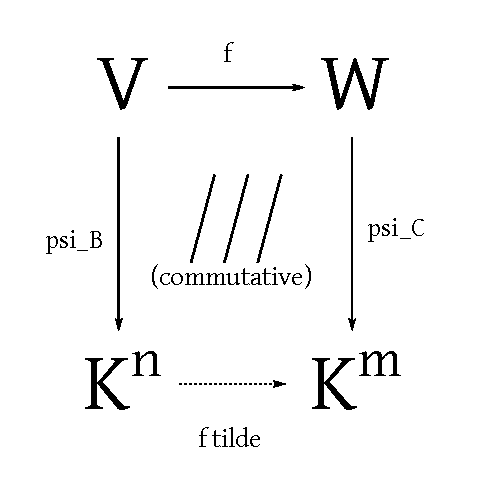
\includegraphics[width=0.3\textwidth]{img/linear_mapping.pdf}
      \caption{Linear mapping in terms of $f$}
      \label{img:lm}
    \end{center}
  \end{figure}
\end{theorem}

\begin{theorem}
  \label{satz-6.52}
  $\Phi_C^B(f)$ is the matrix for which it holds that
  \[ \Phi_C(f(v)) = \Phi_C^B(f) \cdot \Phi_B(v) \]
  \[ f(v)_C = A \cdot (v)_B \]
  \[ S_i(\Phi_C^B(f)) = \Phi_C(f(b_i)) \]
\end{theorem}

\begin{cor}
  \label{corollary-6.53}
  \[
    \Phi_C^B(f) =
    \begin{bmatrix}
      \Phi_C(f(b_1)) & \Phi_C(f(b_2)) & \ldots \\
      \vdots & \vdots & \vdots
    \end{bmatrix}
  \]
  Columns of $\Phi_C^B(f)$ are the coordinate vectors of the images of the base vectors in regards of basis $C$.
\end{cor}
\begin{proof}
  \[
    S_i(\Phi_C^B(f))
    = \Phi_C^B(f) \cdot e_i
    = \Phi_C^B(f) \Phi_B(b_i)
    \overset{\text{Theorem~\ref{satz-6.52} for } v = b_i}{=} \Phi_C(f(b_i))
  \] \[
    e_i = \Phi_B(b_i)
  \]
\end{proof}

\begin{ex}
  \label{ex-6.55}
  \[
    V = \mathbb R^3 \text{ with basis } \left(
      \begin{pmatrix} 1 \\ 1 \\ 1 \end{pmatrix},
      \begin{pmatrix} 1 \\ 0 \\ 1 \end{pmatrix},
      \begin{pmatrix} -1 \\ 1 \\ 1 \end{pmatrix}
    \right) = B
  \] \[
    W = \mathbb R^2 \text{ with basis } \left(
      \begin{pmatrix} 1 \\ 1 \end{pmatrix},
      \begin{pmatrix} 2 \\ 0 \end{pmatrix}
    \right) = C
  \] \[
    f: V \to W
  \] \[
    \begin{pmatrix} x \\ y \\ z \end{pmatrix}
    \mapsto
    \begin{pmatrix}
      x + 3y - z \\
      2y + 3z
    \end{pmatrix}
  \] \[
    \Phi_C^B(f) = \text{?}
  \]
  $i$-th column is image of $b_i$ in basis $C$.

  \begin{align*}
    f(b_1) &= f\begin{pmatrix} 1 \\ 1 \\ 1 \end{pmatrix} = \begin{pmatrix} 3 \\ 5 \end{pmatrix} \\
    f(b_2) &= f\begin{pmatrix} 1 \\ 0 \\ 1 \end{pmatrix} = \begin{pmatrix} 0 \\ 3 \end{pmatrix} \\
    f(b_3) &= f\begin{pmatrix} -1 \\ 1 \\ 1 \end{pmatrix} = \begin{pmatrix} 1 \\ 5 \end{pmatrix}
  \end{align*}
  \[
    \begin{pmatrix}
      3 & 0 & 1 \\
      5 & 3 & 5
    \end{pmatrix}
    = \Phi_{\text{std basis}}^B(f)
  \]

  $\Phi_C(f(b_i)):$ solve $\lambda_1 c_1 + \lambda_2 c_2 = f(b_i)$
  \[
    \begin{pmatrix} C_1 & C_2 \\ \vdots & \vdots \end{pmatrix}
    \cdot
    \begin{pmatrix} \lambda_1 \\ \lambda_2 \end{pmatrix} = f(b_i)
  \]

  \[
    \begin{array}{cc|ccc}
        & 2 & 3 & 0 & 1 \\
      1 & 0 & 5 & 3 & 5 \\
    \hline
      0 & 2 & -2 & -3 & -4 \\
        & 1 & -1 & -\frac32 & -2
    \end{array}
  \] \[
    \leadsto
    \Phi_C^B(f) = \begin{pmatrix}
      5 & 3 & 5 \\
      -1 & -\frac32 & -2
    \end{pmatrix}
  \]


  Test:
  \[ \Phi_C^B(t) \cdot \Phi_B(b_i) = \begin{pmatrix} 5 \\ -1 \end{pmatrix} \]
  \[
    5 \cdot c_1 - c_2 = 5 \cdot \begin{pmatrix} 1 \\ 1 \end{pmatrix} - \begin{pmatrix} 2 \\ 0 \end{pmatrix}
    = \begin{pmatrix} 3 \\ 5 \end{pmatrix} = t \cdot (b_1)
  \]
\end{ex}

\begin{theorem}
  \label{satz-6.54}
  $\Phi_C^B: \Hom(V,W) \to K^{m\times n}$ is linear where $B,C$ are bases of $V, W$.
  Hence,
  \[ \Phi_C^B(\lambda \cdot f + \mu \cdot g) = \lambda \cdot \Phi_C^B(f) + \mu \Phi_C^B(g) \]
\end{theorem}
\begin{proof}
  Will be provided in the practicals for basis elements.
\end{proof}

\begin{theorem}
  \label{satz-6.56}
  Let $B = (b_1, \ldots, b_n)$ be basis of $V$.
  Let $C = (c_1, \ldots, c_m)$ be basis of $W$.
  Let $D = (d_1, \ldots, d_p)$ be basis of $Z$.
  \[ f: V \to W \qquad g: W \to Z \quad \text{ linear} \]
  \[ \Rightarrow \Phi_D^B (g \circ f) = \Phi_D^C(g) \cdot \Phi_C^B(f) \]
\end{theorem}

\begin{figure}[!h]
  \begin{center}
    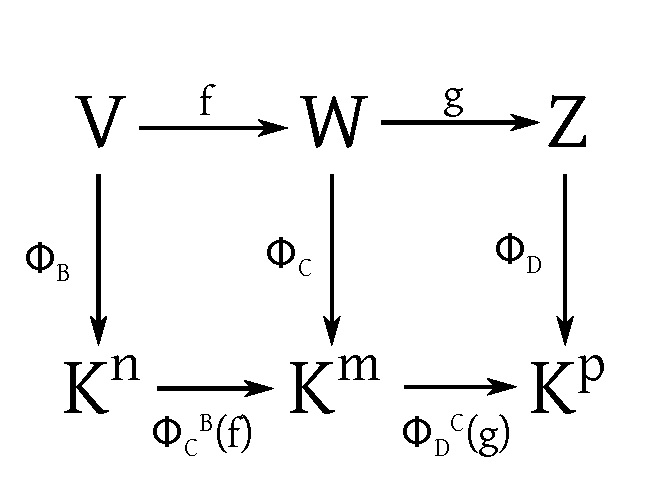
\includegraphics[width=0.3\textwidth]{img/two_linear_mappings.pdf}
    \caption{Mapping $f$ and $g$}
    \label{img:two-linear-mappings}
  \end{center}
\end{figure}

\begin{proof}
  \[ ((g \circ f) (v))_D \overset!= \Phi_D^C(g) \cdot  \Phi_C^B(f) \circ (v)_B \]
  \begin{align*}
    \Phi_D((g \circ f)(v)) &= \Phi_D(g(f(v))) \\
      &= \Phi_D^C(g) \cdot \Phi_C(f(v)) \\
      &= \Phi_D^C(g) \cdot \Phi_C^B(f) \cdot \Phi_B(v)
  \end{align*}
\end{proof}

\meta{lecture}{26th of January 2016}{Wolfgang Wöss}

\[ V \cong K^m \qquad W \cong K^m \]
\[ B = (b_1, \ldots, b_n)  \qquad  C = (c_1, \ldots, c_n)  \]

\begin{figure}[t]
  \begin{center}
    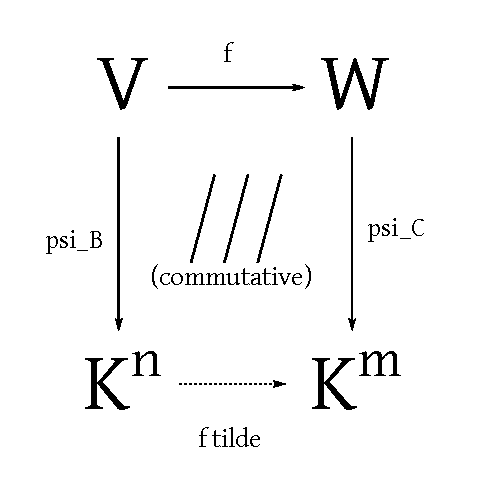
\includegraphics[width=0.3\textwidth]{img/linear_mapping.pdf}
    \caption{Linear mapping in terms of $f$}
    \label{img:lm}
  \end{center}
\end{figure}

\[ \Phi_B:  V \to K^n \]
\[ v \mapsto \begin{pmatrix} \lambda_1 \\ \vdots \\ \lambda_n \end{pmatrix} \]

\[ \Phi_C: W \to K^m \]
\[ w \mapsto \begin{pmatrix} \mu_1 \\ \vdots \\ \mu_m \end{pmatrix} \]

\[ v = \sum_{j=1}^n \lambda_j b_j \]
\[ w = \sum_{i=0}^m \mu_i c_i \]
\[ \tilde{f} = \Phi_B \circ f \circ \Phi_B^{-1} = f_A \]

$m\times n$ matrix:
\[ A = \Phi_C^B(f) \]
\[
  \Phi_C^B(f) = \left(
    \underbrace{\Phi_C(f(b_1))}_{\text{1st column}},
    \Phi_C(f(b_2)),
    \ldots,
    \underbrace{\Phi_C(f(b_n))}_{\text{$n$-th column}}
  \right)
\]
\[ f \mapsto \Phi_C^3(f) \]
\[ \Hom(V, W) \to K^{m\times n} \]
is the vector space of $m\times n$ matrices over $K$.

\begin{theorem}
  \label{satz-6.57}
  \begin{enumerate}
    \item
      Given
      \[ V \cong K^m \qquad W \cong K^m \]
      \[ B = (b_1, \ldots, b_n)  \qquad  C = (c_1, \ldots, c_n)  \]
      \[ \Phi_B:  V \to K^n \qquad \Phi_C: W \to K^m \]
      Then
      \[ \rank{\Phi_C^B(f)} = \dim{\underbrace{\image(f)}_{f(r) \subset W}} \]
    \item
      $f$ is an isomorphism if and only if $m = n$ and $\Phi_C^B(f)$ is regular.
      So $\Phi_B^C(f^{-1}) = \Phi_C^B(f)^{-1}$ holds.
  \end{enumerate}
\end{theorem}
\begin{proof}
  \begin{enumerate}
    \item
      \[ V = L(b_1, \ldots, b_n) \]
      \[ \image{V} = L(f(b_1), \ldots, f(b_n)) \]
      \[ \cong \Phi_C(f(b_1), \ldots, f(b_n)) \]
      \[ = L(\underbrace{\Phi_C(f(b_1)), \ldots, \Phi_C(f(b_n)}_{\text{columns of } \Phi_C^B}) \]
      So,
      \[ \dim{\image{V}} = \dim{L(\Phi_C(f(b_1)), \ldots, \Phi_C(f(b_n)))} = \rank(\Phi_C^B) \]
      Why is $\Phi_C$ an isomorphism? $\Phi_C: W \to K^m$ (bijective and linear).
      \[ U = L(f(b_1), \ldots, f(b_n)) \]
      \[ \left.\Phi_C\right|_U: U \to \Phi_C(U) \subset K^m \]
    \item
      $m = n$ is trivial.

      \[ f \text{ is an isomorphism } \Leftrightarrow \image{f} = W \]
      \[ \Leftrightarrow \dim{\image{f}} = n \]
      \[
        \Leftrightarrow
        \rank\left(\underbrace{\Phi_C^B(f)}_{n\times n \text{ matrix}}\right)
        = n \Leftrightarrow \underbrace{\Phi_C^B(f)}_{\text{regular}}
      \] \[
        \Phi_C^B(f) \cdot \Phi_B^C(f^{-1})
          \overset{\text{Theorem~\ref{satz-6.56}}}{=} \Phi_C^C(f \cdot f^{-1})
          = \Phi_C^C(\text{id}_W)
          = I_n
      \]
  \end{enumerate}
\end{proof}

\index[English]{Basis transformation matrix}
\index[German]{\foreignlanguage{ngerman}{Basistransformationsmatrix}}
\begin{defi}
  \label{satz-6.58}
  \[ V \cong K^n \]
  Bases $B = (b_1, \ldots, b_n)$ and $B' = (b'_1, \ldots, b'_n)$.
  \begin{enumerate}
    \item
      \[ \Phi_{B'}^B(\text{id}_V) \leftrightarrow \Phi_{B'} \circ \Phi_B^{-1} \]
      \[ \Phi_{B'}^B(\text{id}_V) = T_{B'}^B \]
      \begin{center}
        \enquote{basis transformation matrix}
      \end{center}
      So,
      \[ T_{B'}^B = (\underbrace{\Phi_B(b_1)}_{\text{column $1$}}, \ldots, \underbrace{\Phi_B(b_n)}_{\text{column $n$}}) \]
    \item $T_{B'}^B$ is invertible and (follows from Theorem~\ref{satz-6.57})
      \[ \left(T_{B'}^B\right)^{-1} = T_B^{B'} \]
    \item
      Given
      \[ V \cong K^m \qquad W \cong K^m \]
      \[ B = (b_1, \ldots, b_n)  \qquad  C = (c_1, \ldots, c_n)  \]
      \[ \Phi_B:  V \to K^n \qquad \Phi_C: W \to K^m \]
      Then we have new bases
      \[ B' = (b_1', \ldots, b_n') \text{ of } V \]
      \[ C' = (c_1', \ldots, c_n') \text{ of } W \]
      \begin{align*}
        \Phi_{C'}^B(f) &=
          \underbrace{T_{C'}^C}_{m \times m} \cdot
          \underbrace{\Phi_C^B(f)}_{m\times n} \cdot
          \underbrace{T_B^{B'}}_{n\times n} \\
        &= \left(T_C^{C'}\right)^{-1} \cdot \Phi_C^B(f) \cdot T_B^{B'}
      \end{align*}
      Figure~\ref{img:other-2-lin-maps} follows from Theorem~\ref{satz-6.56}.
      \begin{figure}[!h]
        \begin{center}
          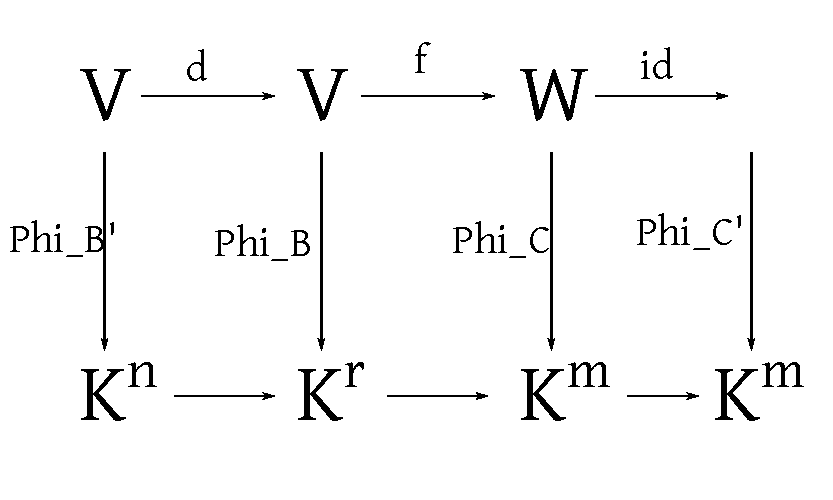
\includegraphics[width=0.4\textwidth]{img/other_two_linear_mappings.pdf}
          \caption{This structure follows from Theorem~\ref{satz-6.56}}
          \label{img:other-2-lin-maps}
        \end{center}
      \end{figure}
  \end{enumerate}
\end{defi}

\begin{cor}
  \begin{enumerate}
    \item
      Matrix representations $\Phi_C^B(f)$ and $\Phi_{C'}^{B'}(f)$ of a linear mapping
      $f: V \to W$ are pairwise equivalent.
    \item
      Two matrix representations $\Phi_B^B(f)$ and $\Phi_{B'}^{B'}(f)$ of $f \in \End(V)$
      are pairwise similar
      \[ \Phi_B^B(f) = \left(T_B^B\right)^{-1} \Phi_B^{B}(f) T_B^{B'} \]
    \item
      $f$ as previously. $K \cong V \to W \cong K^n$. $B = (b_1, \ldots, b_n)$ and $C = (c_1, \ldots, c_n)$.

      Then bases $B$ of $V$ and $C$ of $W$ exist such that
      \[ \Phi_C^B(f) = I_{m \times n}^{(r)} \]
      Hence we have $r$ diagonal ones.
  \end{enumerate}
\end{cor}

\clearpage
\begin{otherlanguage}{ngerman}
\printindex[German]
\end{otherlanguage}
\printindex[English]

\end{document}
